\chapter{Experiments}
\label{chap:experiments}
This chapter presents the experiments designed to evaluate the system described in chapter \autoref{chap:methods}.
The chapter is structured as follows: \autoref{sec:exp-setup} specifies the setup used for the class incremental learning task; \autoref{sec:exp-cil} discusses the experiments related to the CIL model and \autoref{sec:exp-det} those related to the logo detector; \autoref{sec:exp-kd} describes the experiments relative to the KD; finally, \autoref{sec:exp-end2end} presents the results of experiments combining the logo detector with the CIL classifier.

\section{Setup}
\label{sec:exp-setup}
The developed system is tested considering two different CIL setups: in the first setup, the system is tested on a subset of 100 classes out of the total 2993 in the dataset; in the second setup, the model's scaling capabilities are tested considering the entire dataset. Specifically, the CIL configuration is the following:
\begin{enumerate}
    \item \textbf{100 Classes}: 100 classes are extracted from the initial dataset. For the experiments, a distinction is made between the case in which these classes are extracted randomly or are taken the 100 classes with the highest number of images.
    
    Out of these 100 classes, 30 are used for the initial task, then the remaining 70 classes are added 10 at a time through 7 incremental learning iterations.

    \item \textbf{2993 Classes (entire dataset)}: for experiments which consider the entire dataset, the first 1000 classes are used for the initial task, then follows 8 iterations of incremental learning, each adding 250 new classes.
\end{enumerate}

The train, validation and test set are built from the individual classes. For each of these, the instances are divided as follows:
\begin{itemize}
    \item \textbf{Train set}: 70 \%
    \item \textbf{Validation set}: 10 \%
    \item \textbf{Test set}: 20 \%
\end{itemize}


\section{Classifier: CIL model}
\label{sec:exp-cil}
Top-k accuracy is used to evaluate the performance of the CIL model, focusing on cases with $k=1$ and $k=5$.
Using this performance metric, a classification is considered correct if the label is present among the first $k$ predictions to which the model assigns the highest probability. Thus, the accuracy is calculated as the percentage of the correct predictions.

\subsection{100 Classes}
\subsubsection{100 Classes randomly sampled}
For the first experiments, the 100 classes are randomly sampled from the 2993 classes in the dataset, then the classifier is evaluated on the test set according to the CIL setup described in \autoref{sec:exp-setup}. 

As detailed in \autoref{sec:der-algorithm}, the DER algorithm saves some examples of the 'old' classes and reuses these examples during incremental learning iterations. In the following experiments, the memory dedicated to each old class is of 100 samples.

The first group of experiments aims to compare two types of architecture: ResNet-34 and ResNet-50. In addition, the cases where CNNs are pre-trained on ImageNet or not are also considered. For these experiments, the optimizer is SGD and neither regularization of the model via the dropout layer nor data augmentation is used.

The results of the experiments in picture \autoref{fig:exp1} and table \autoref{table:exp1}, reporting the top-1 and top-5 accuracy of the models at varying CIL tasks on the test set, show that pre-trained CNNs perform better, but there is not much difference between ResNet-34 and ResNet-50. For this reason, the architecture chosen for the experiments to follow is ResNet-34, so as to have a slightly smaller network than ResNet-50, and the network is pre-trained on ImageNet.

\begin{figure}[H]
    \centering
	\subfloat[\centering Top-1 accuracy]{{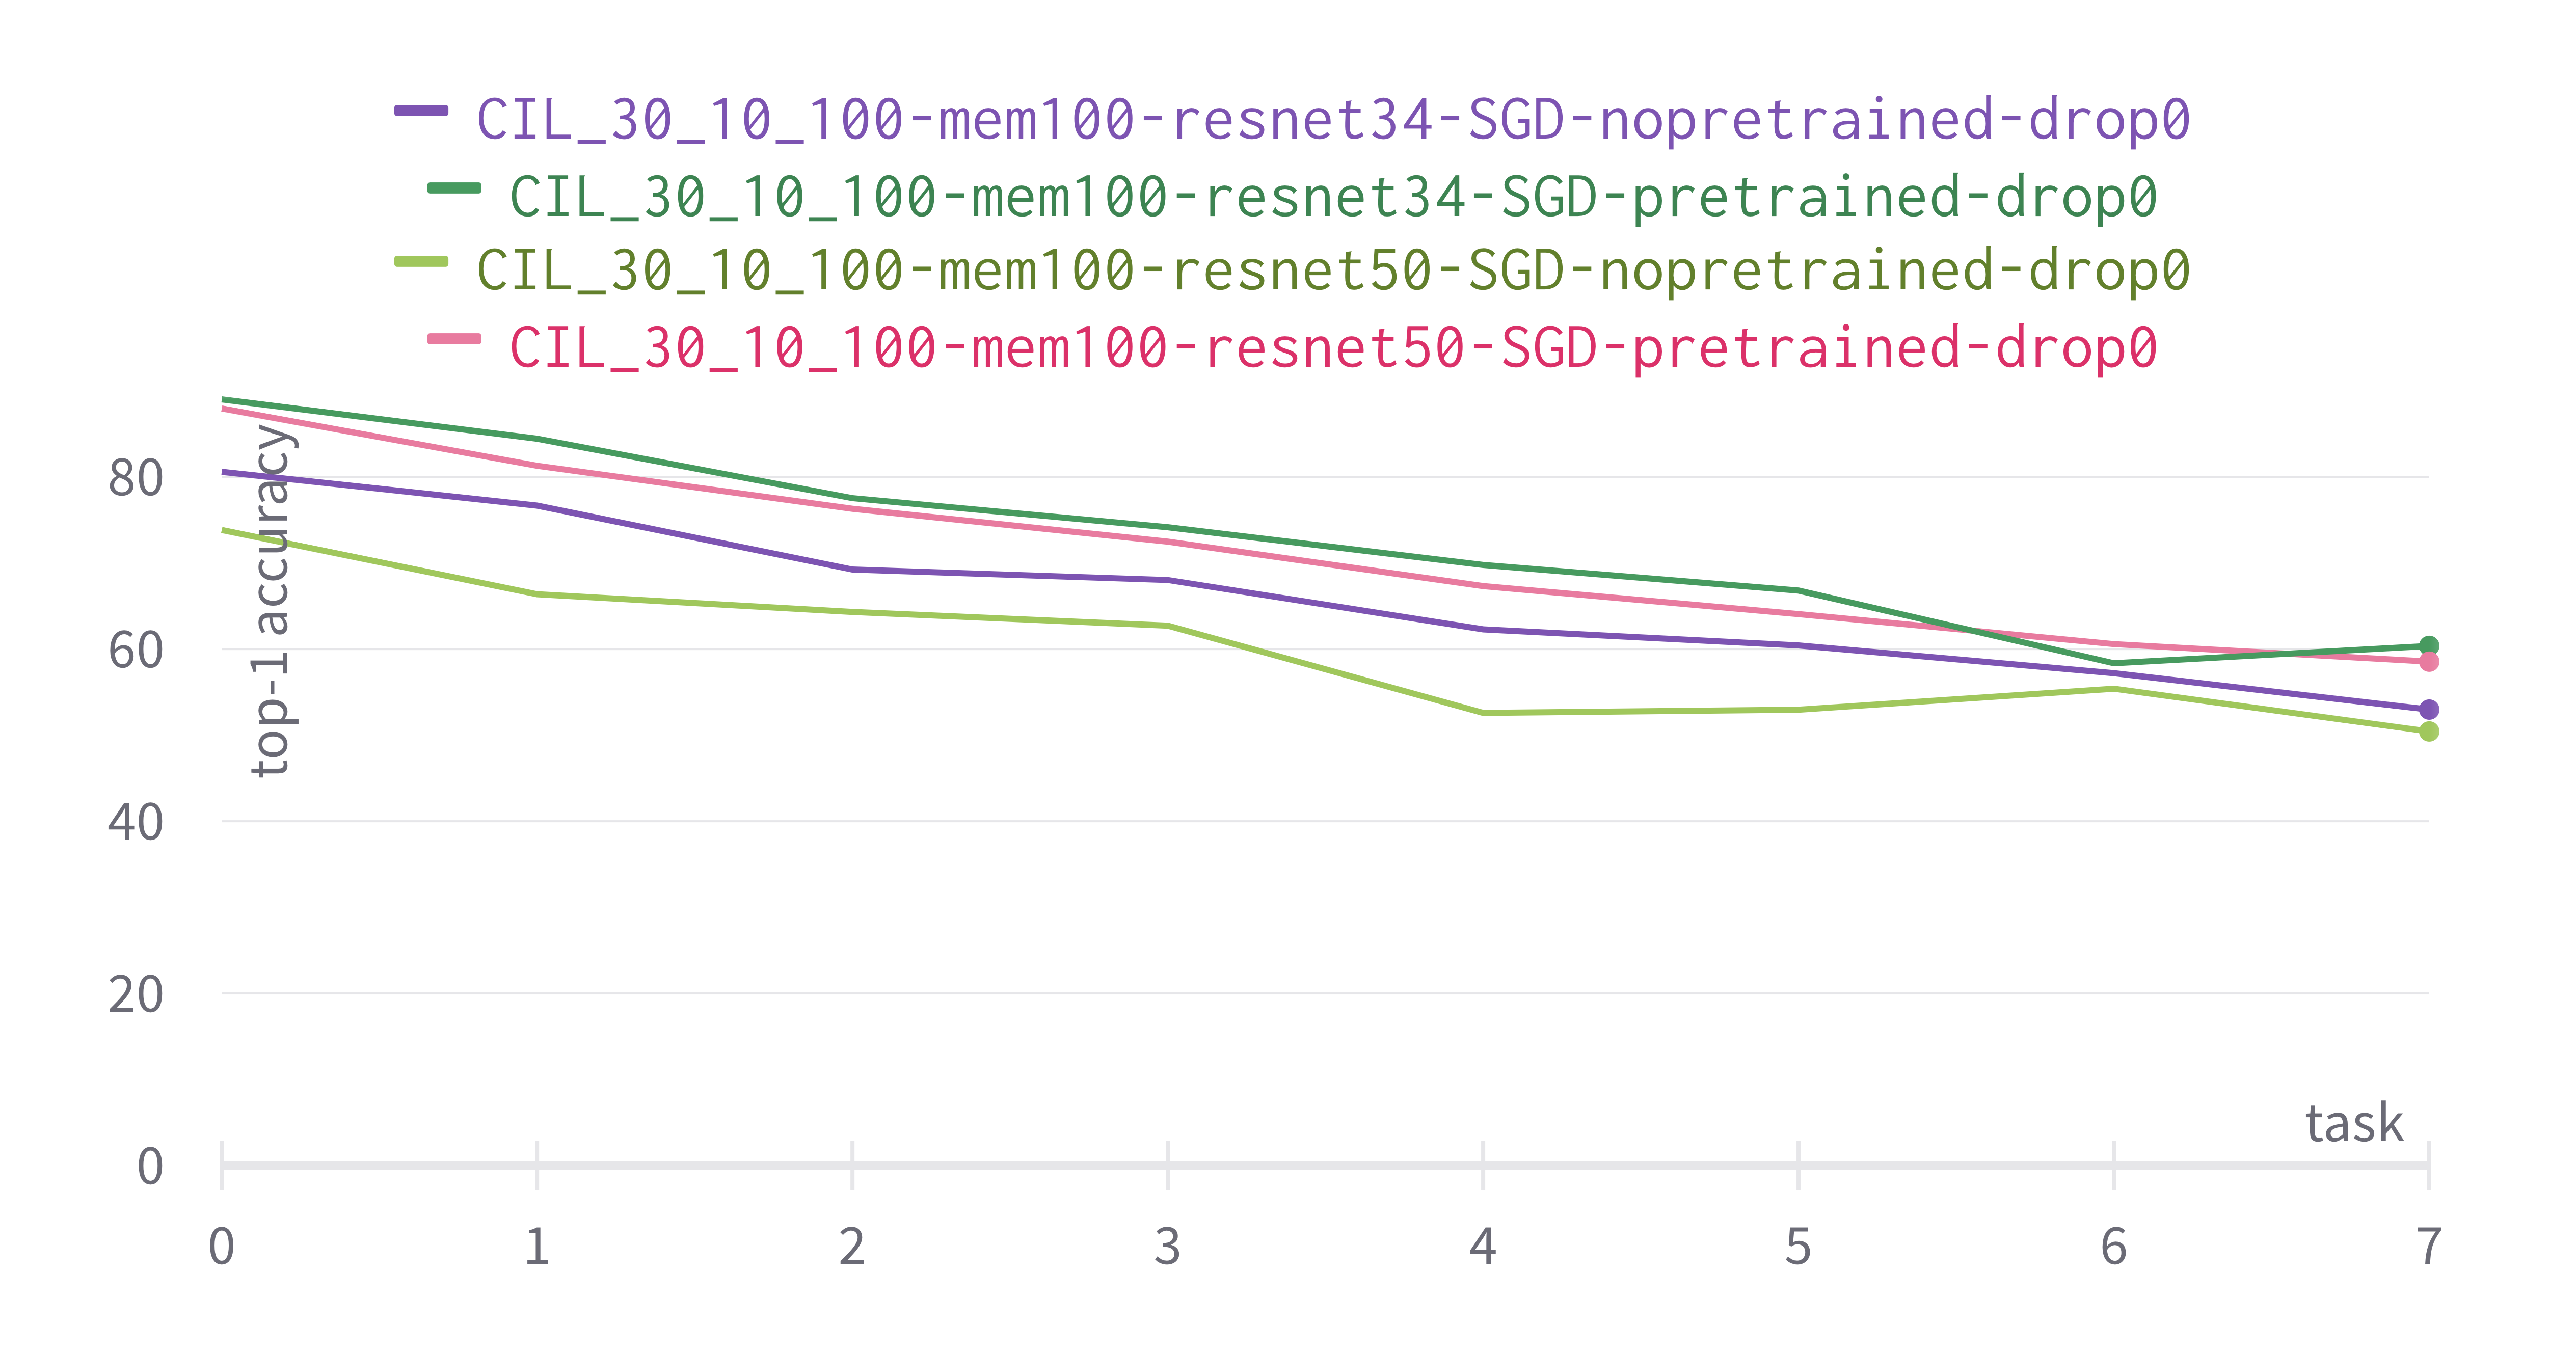
\includegraphics[width=0.80\textwidth]{images/exp/exp1-top1.png} }}%
    \qquad
    \subfloat[\centering Top-5 accuracy]{{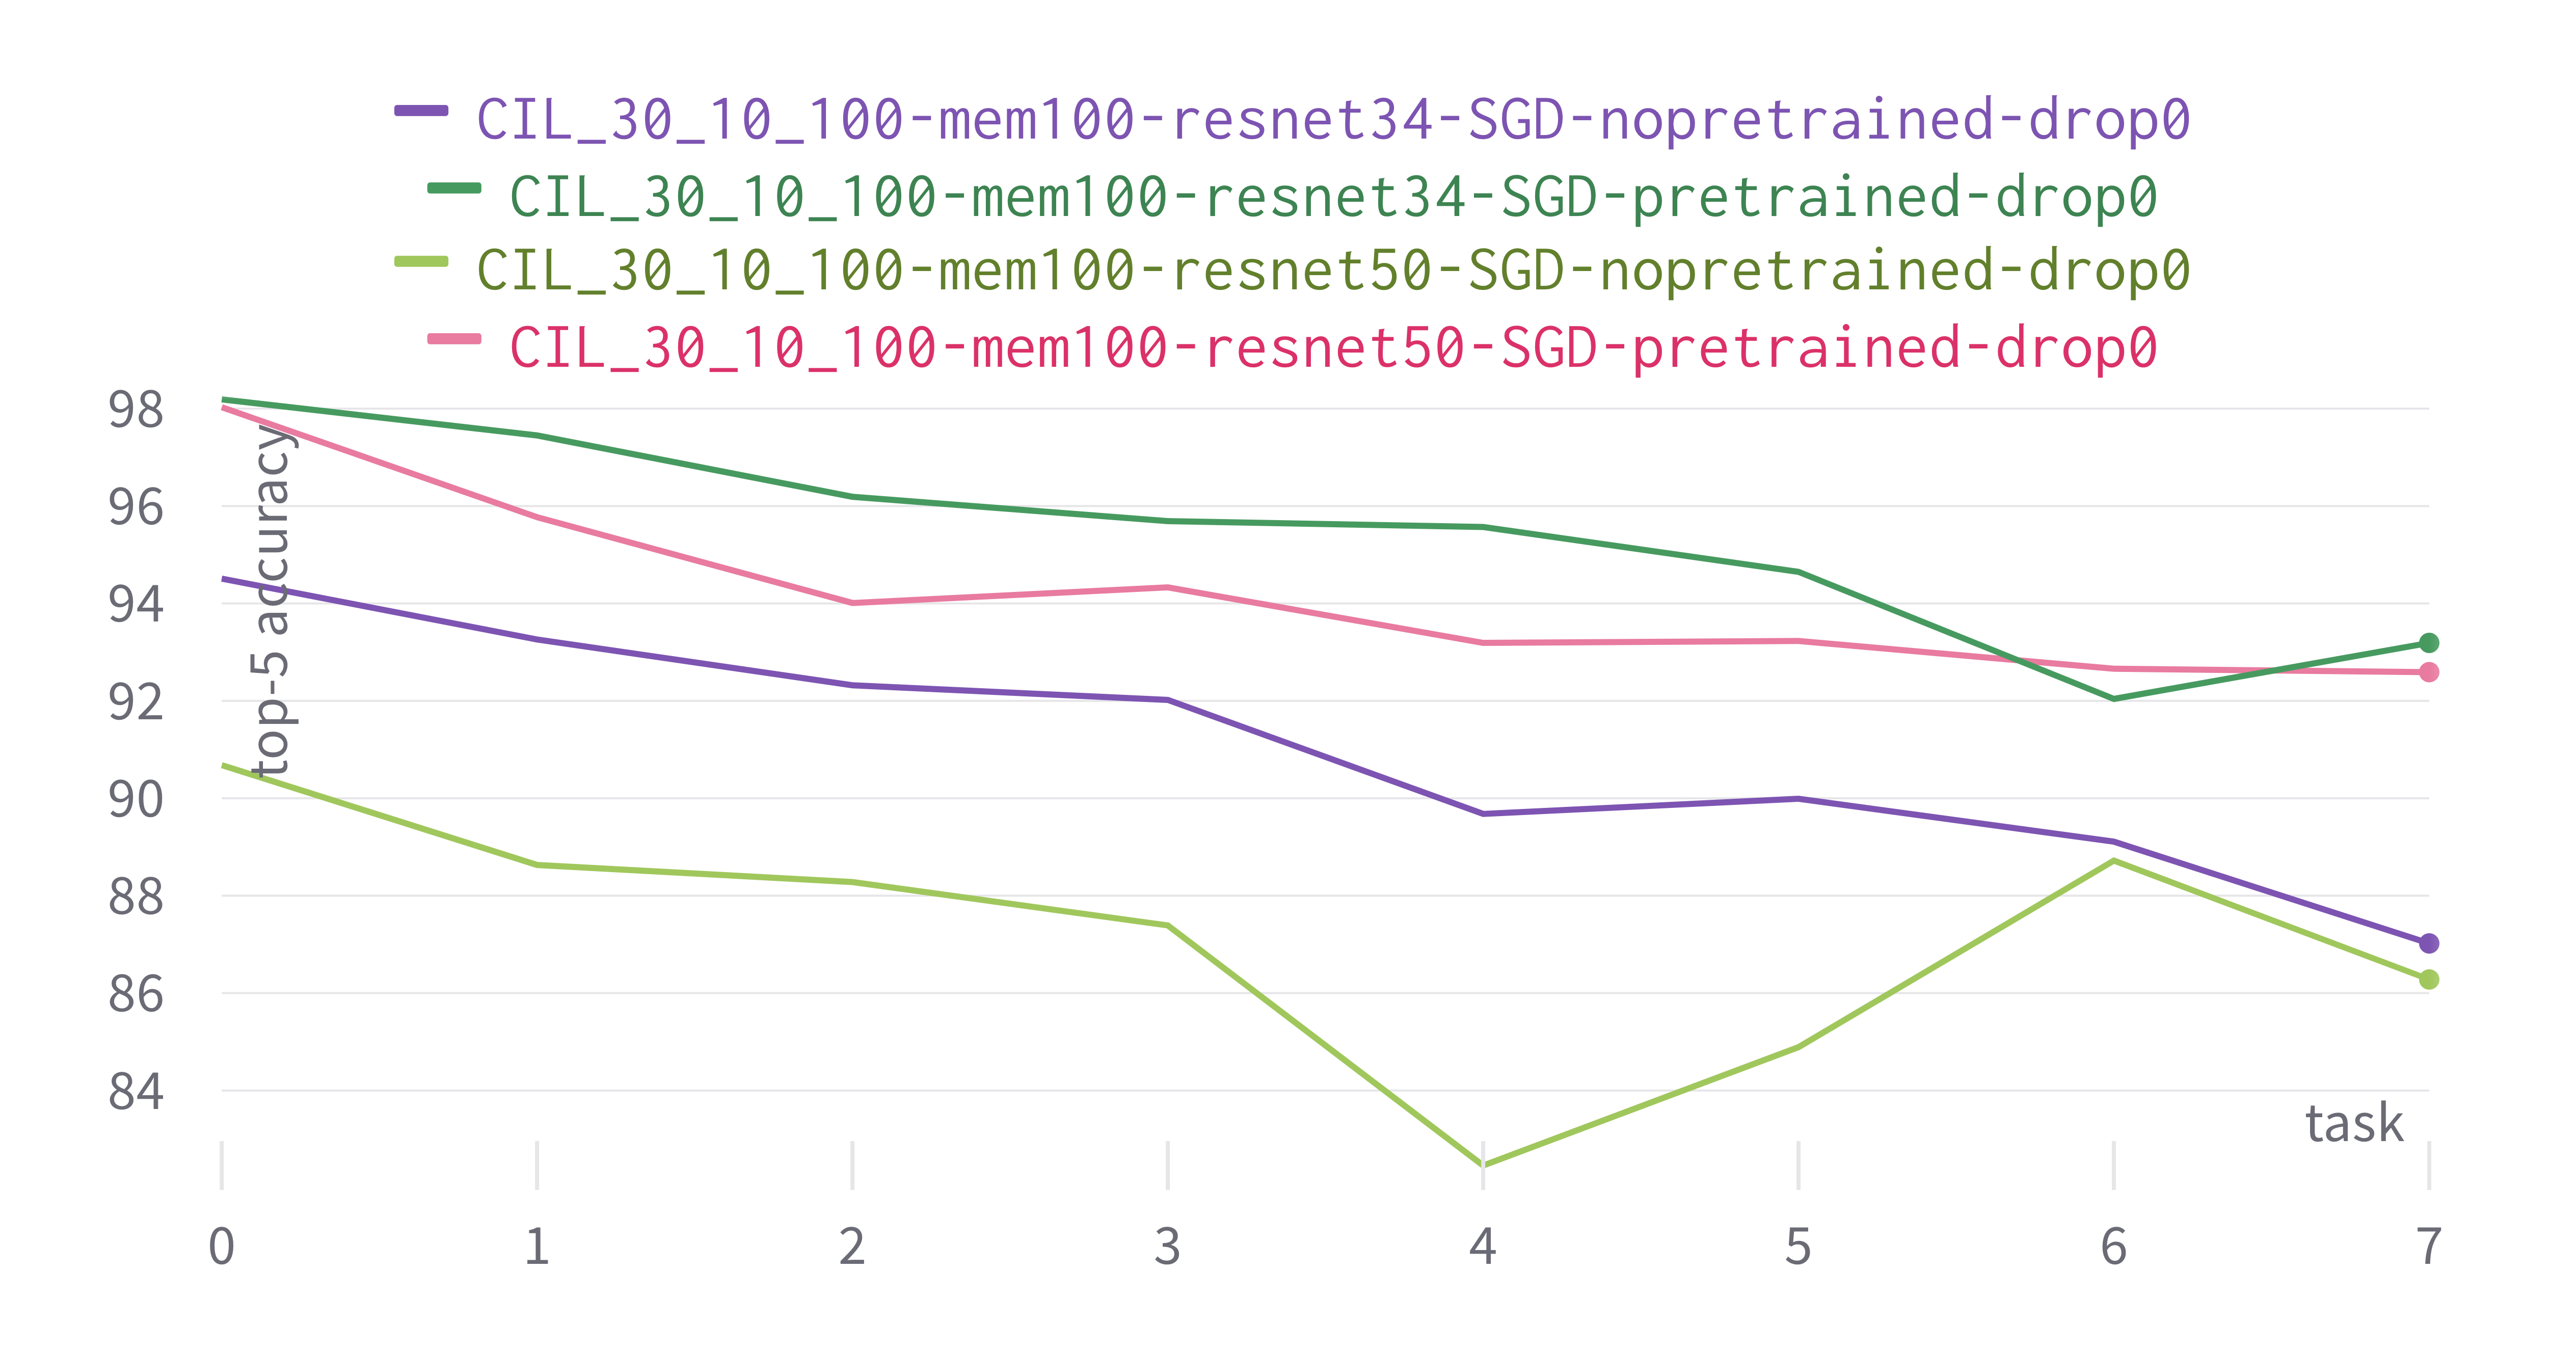
\includegraphics[width=0.80\textwidth]{images/exp/exp1-top5.png} }}%
    \caption{Top-1 and Top-5 accuracy of the models at varying CIL tasks on the test set.}%
	\label{fig:exp1}%
\end{figure}

\begin{table}[H]
    \centering
    \centerline{
    \begin{tabular}{c|c|c|c|c}
        \hline
        \textbf{Model} &
        \textbf{Backbone} &
        \textbf{Pre-trained} &
        \textbf{Top-1} & 
        \textbf{Top-5} \\
        \textbf{name} &
        &
        &
        \textbf{acc. (\%)} & 
        \textbf{acc. (\%)} \\
        \hline
        \hline
resnet34-SGD-nopretrained-drop0 &ResNet-34&no& 52.97 & 87.02\\
resnet34-SGD-pretrained-drop0 &ResNet-34&yes& \textbf{60.37} & \textbf{93.19}\\
resnet50-SGD-nopretrained-drop0 &ResNet-50&no& 50.43 & 86.28\\
resnet50-SGD-pretrained-drop0 &ResNet-50&yes& 58.54 & 92.59\\
        \hline        
    \end{tabular}}
    \caption{Top-1 and Top-5 accuracy of the models at task 7.}
    \label{table:exp1}
\end{table}


Other useful insights can be derived from the training history of a task (e.g. Task 7) which reports the top-1 accuracy on the training and validation set. In fact, as we can see from \autoref{fig:exp1-train_val} the accuracy on the training set is much higher than the validation set, which is a clear sign of overfitting of the model.

\begin{figure}[H]
    \centering
    \subfloat[\centering Accuracy on the training set]{{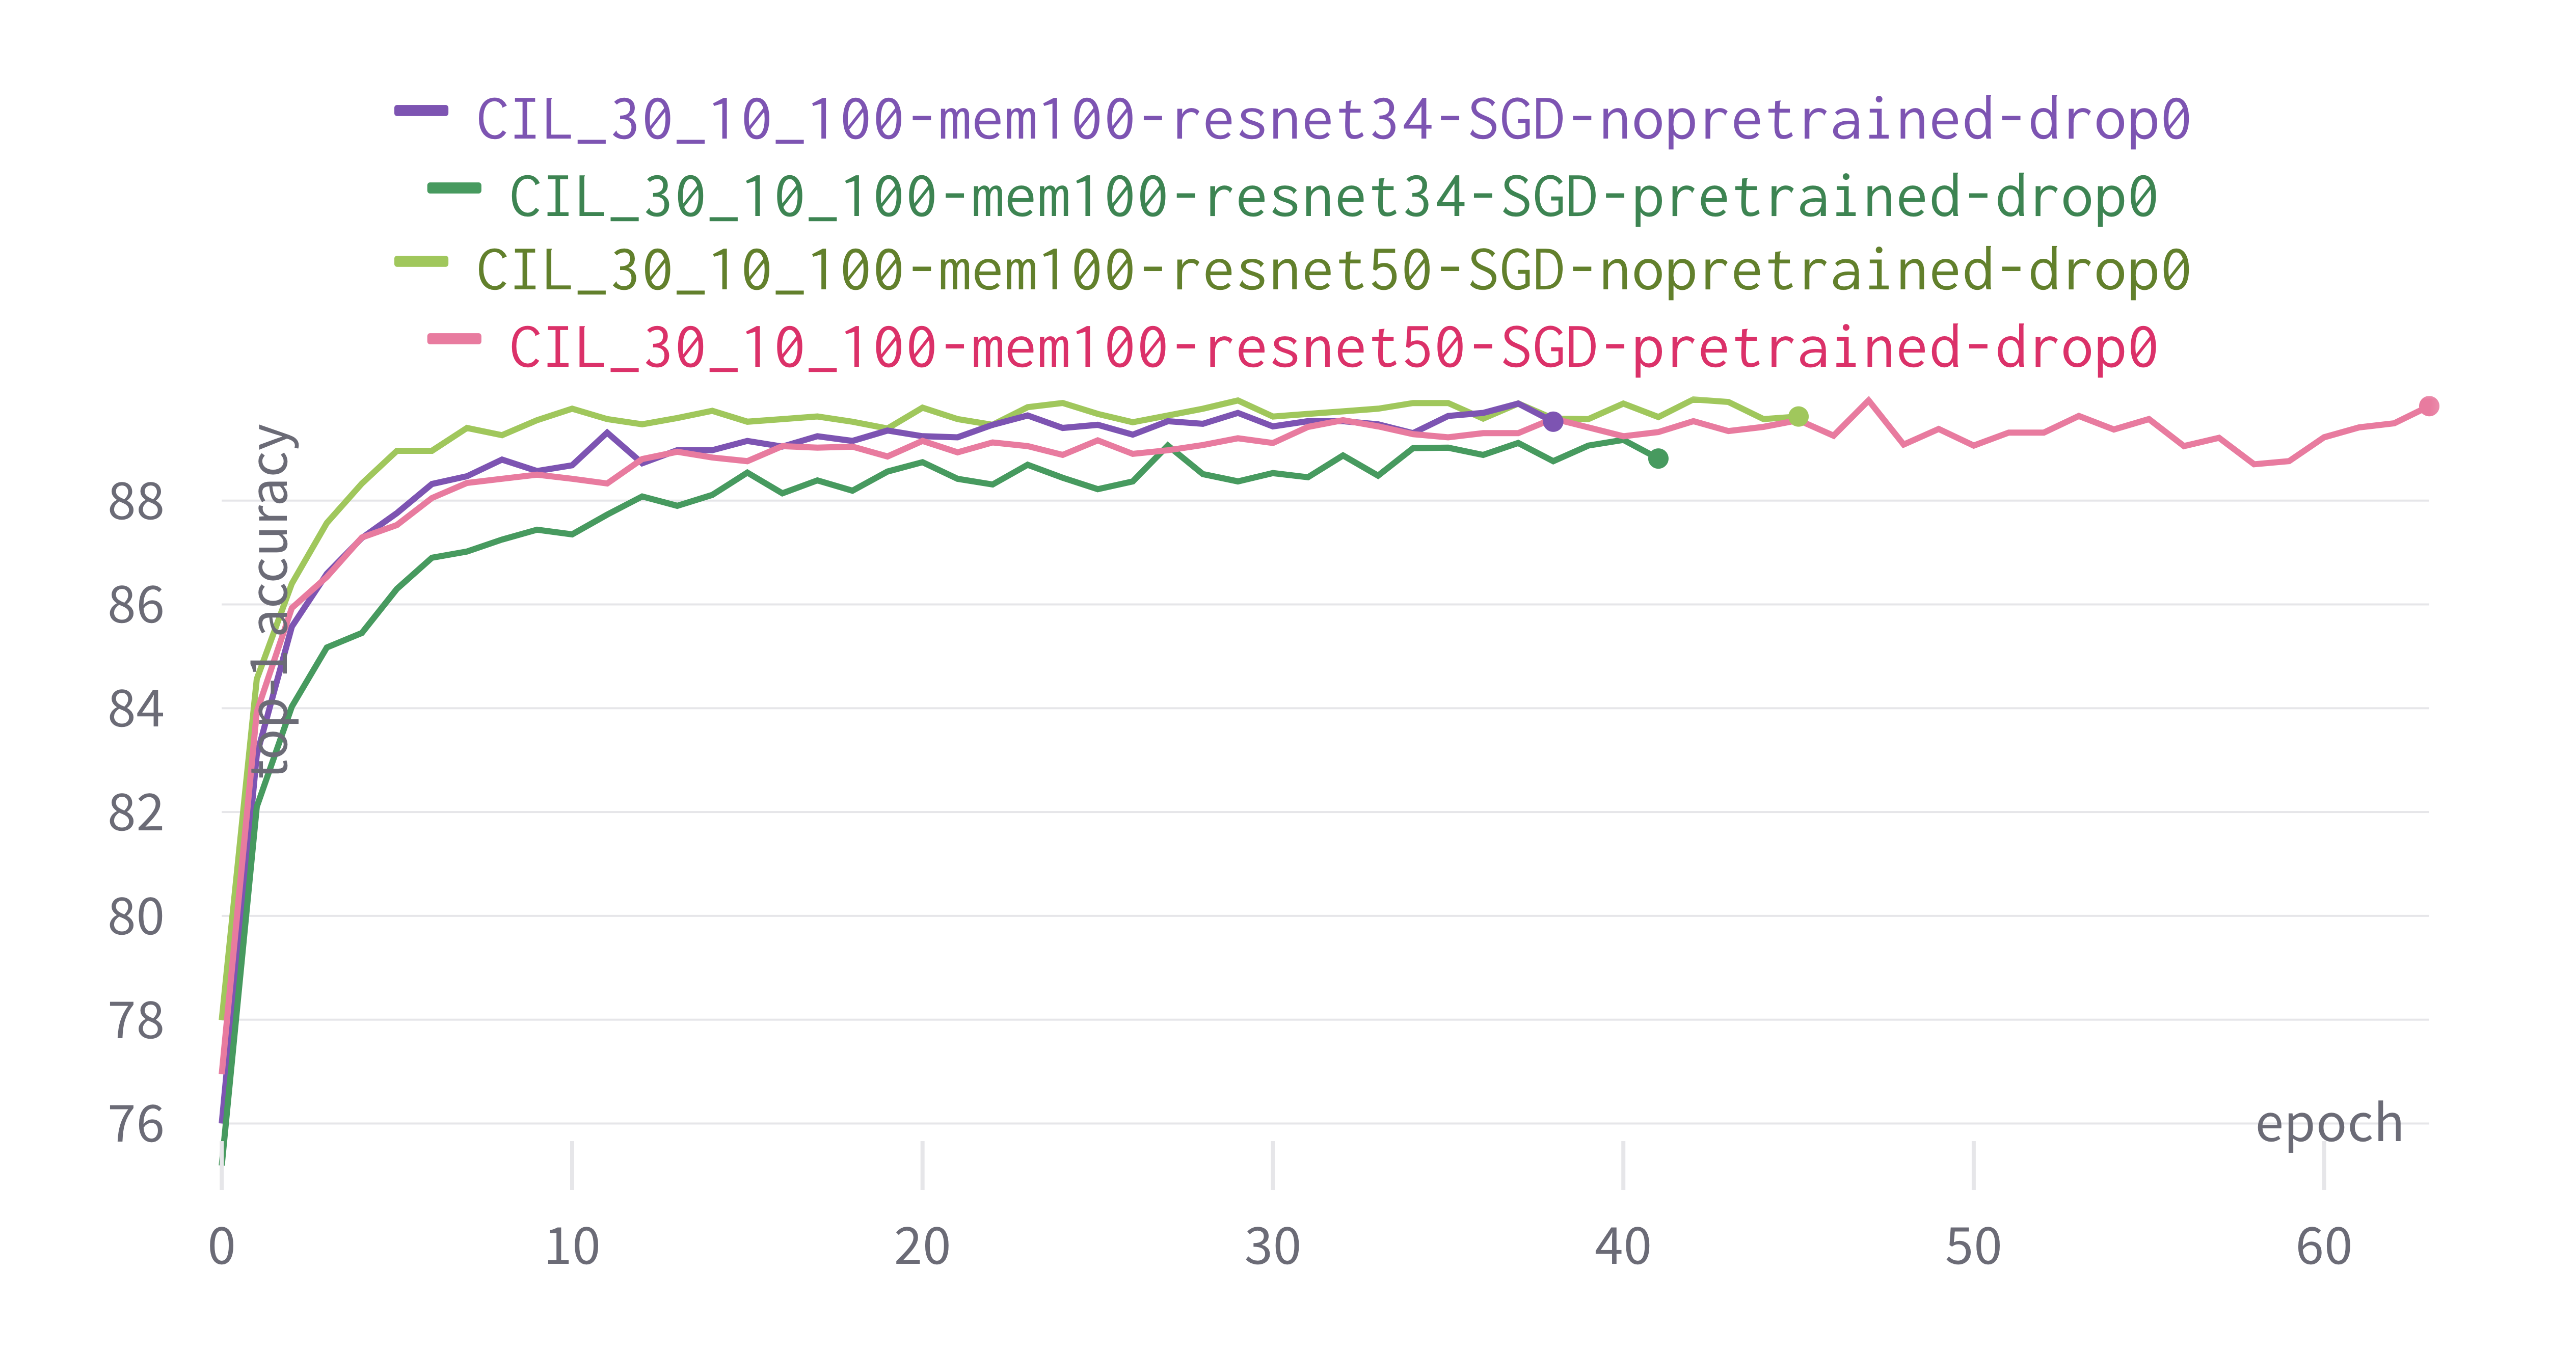
\includegraphics[width=0.80\textwidth]{images/exp/exp1-train.png} }}%
    \qquad
    \centering
    \subfloat[\centering Accuracy on the validation set]{{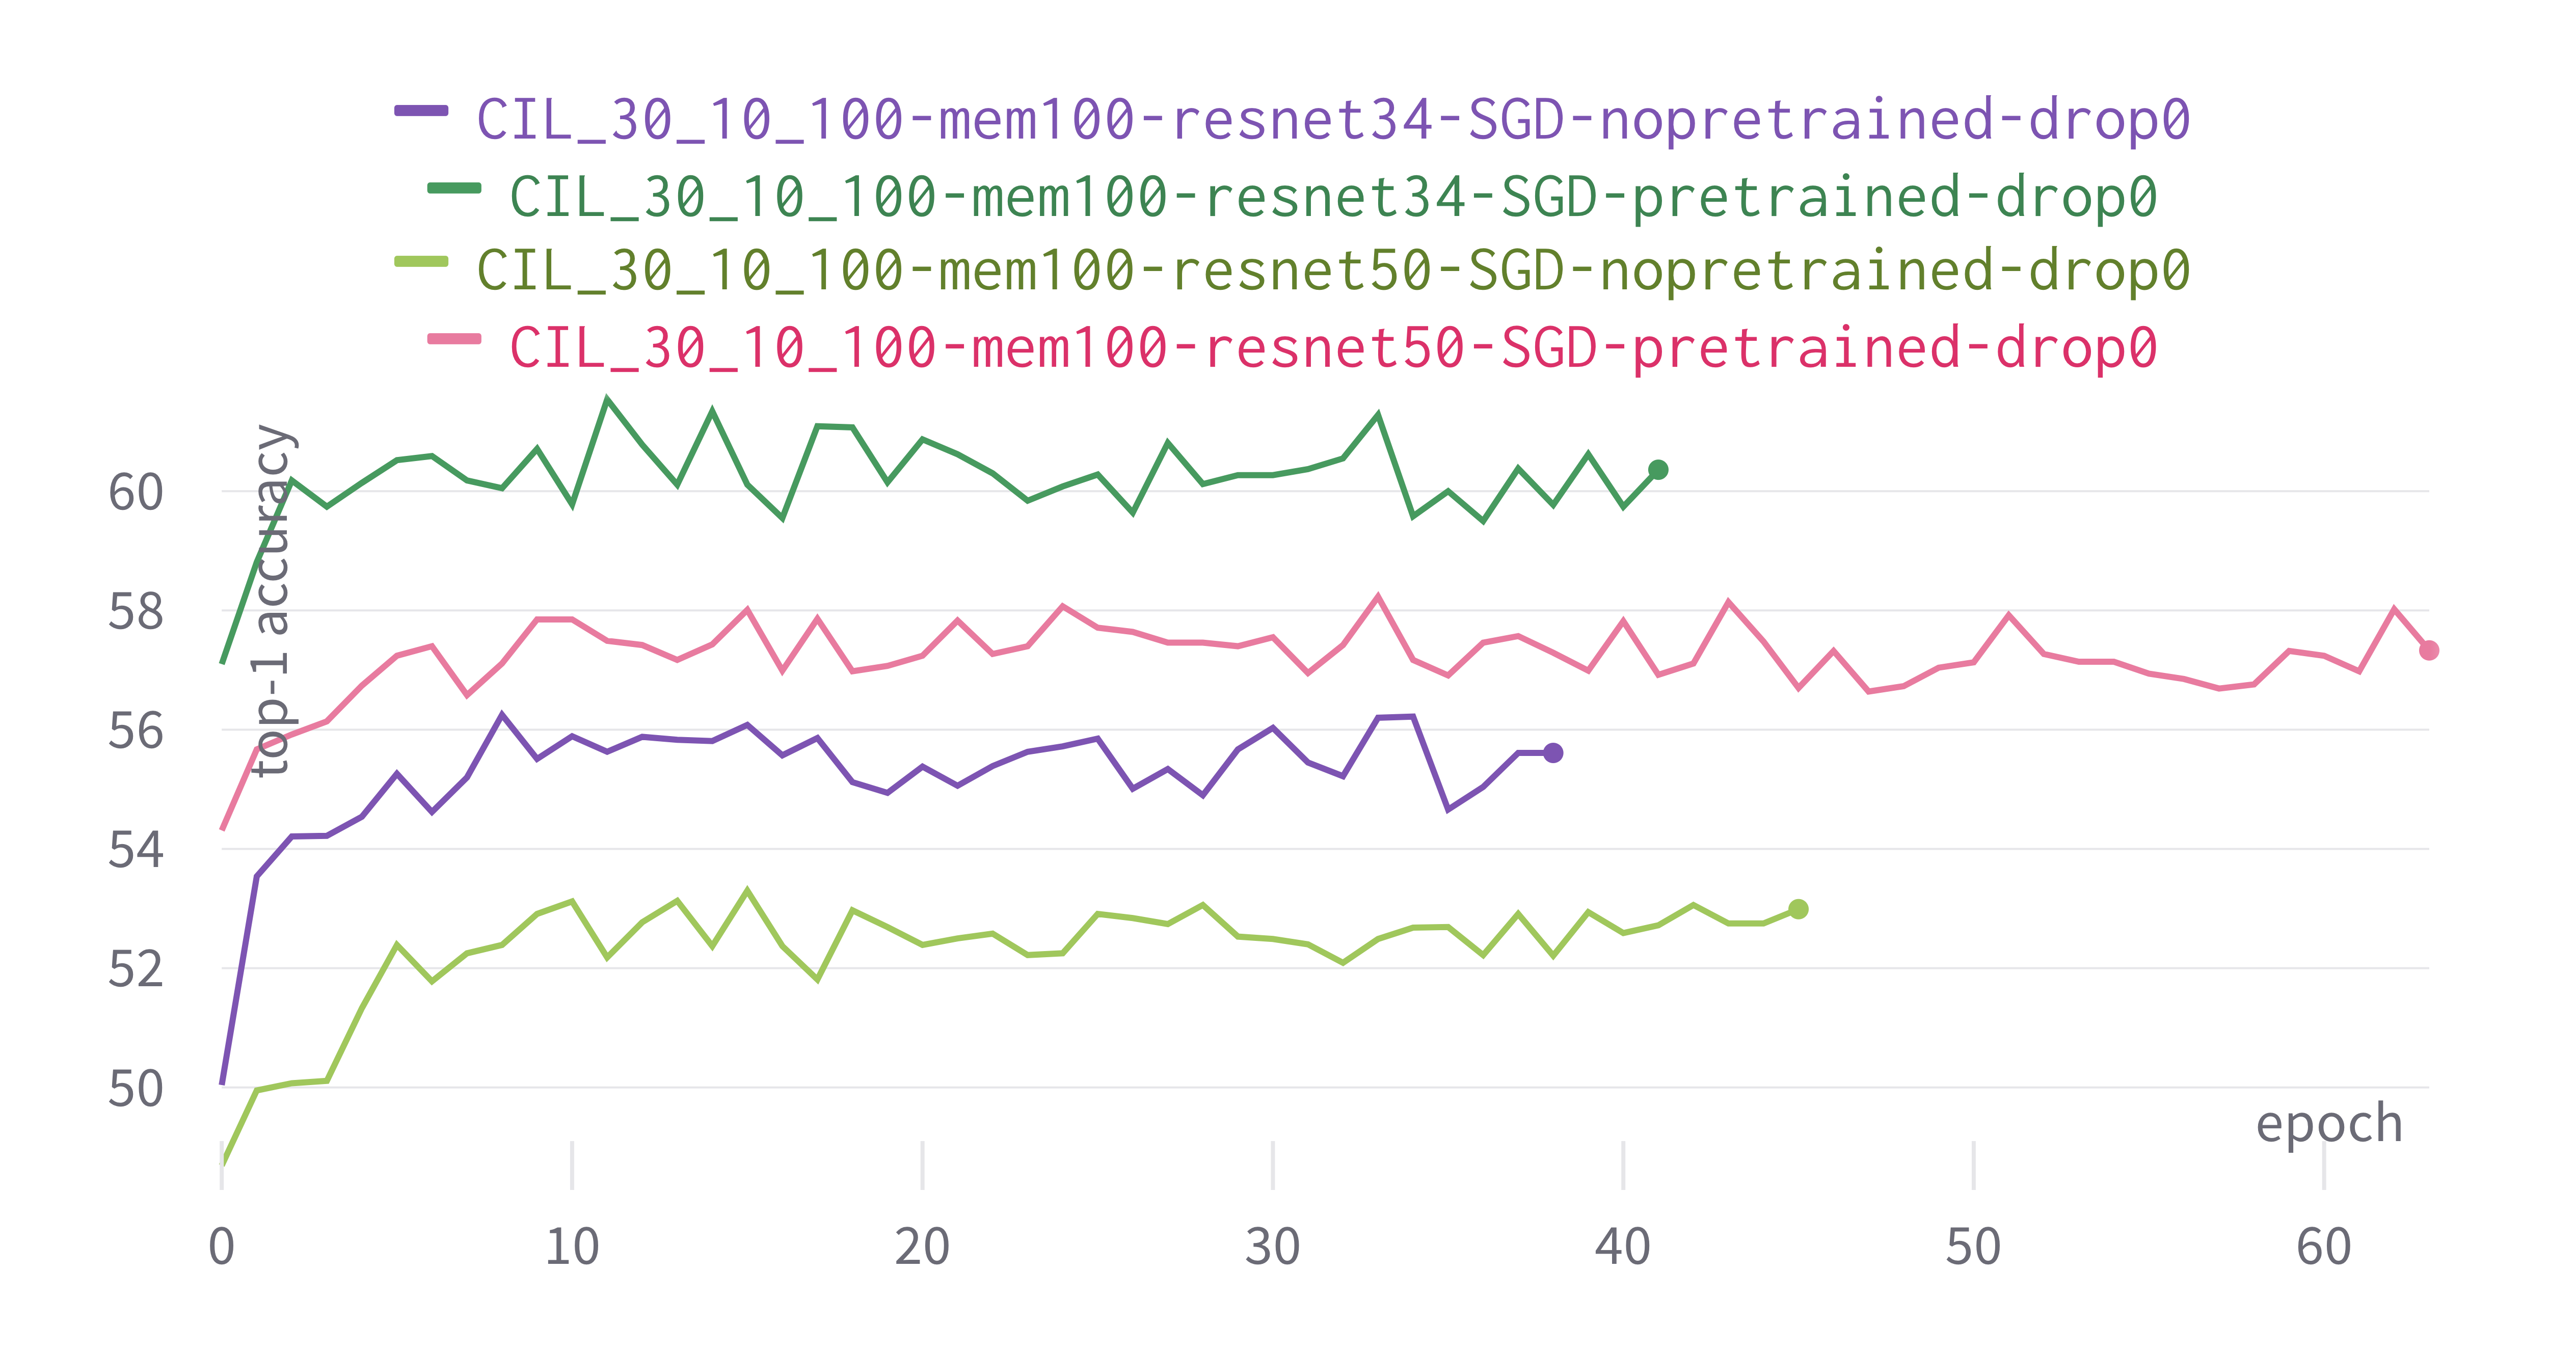
\includegraphics[width=0.80\textwidth]{images/exp/exp1-val.png} }}%
    \caption{Comparison of the accuracy at each training epoch at task 7 between the training and validation set.}%

        \label{fig:exp1-train_val}%
\end{figure}

\newpage
\subsubsection{Regularization and data augmentation}
Following the analysis discussed above, it is necessary to regularize the model.
To do so, the next experiments are performed using the dropout layer (see \autoref{sec:methods-dropout}) and data augmentation (see \autoref{sec:methods-augment}). As said before, the backbone of each model is ResNet-34 and each one is pre-trained on ImageNet.

As expected, the performance at each task is higher than before, as shown in \autoref{fig:exp2}. Analyzing \autoref{fig:exp2-train_val}, the accuracy on the train and validation set at task 7 (the same as before), the training accuracy is lower than models without regularization, but the validation accuracy is higher. This is a sign that the regularization works as intended.

As shown in \autoref{table:exp2}, the top-1 accuracy of the best regularized model which adopting data augmentation is 7\% higher than that without regularization and data augmentation.


\begin{table}[H]
    \centering
    \centerline{
    \begin{tabular}{c|c|c|c|c}
        \hline
        \textbf{Model} &
        \textbf{Data} &
        \textbf{Dropout} &
        \textbf{Top-1} & 
        \textbf{Top-5} \\
        \textbf{name} &
        \textbf{augm.} &
        \textbf{rate} &
        \textbf{acc. (\%)} & 
        \textbf{acc. (\%)} \\
        \hline
        \hline
SGD-nopretrained-drop0 &no&0.0& 52.97 & 87.02\\
SGD-pretrained-drop0 &no&0.0& 60.37 & 93.19\\
\hline
SGD-pretrained-drop0.1-augmented&yes&0.1&	67.17&\textbf{98.15}\\
SGD-pretrained-drop0.3-augmented&yes&0.3&\textbf{67.28}&	97.3\\
SGD-pretrained-drop0.5-augmented&yes&0.5&65.57&	96.24\\
        \hline        
    \end{tabular}}
    \caption{Regularized models with data augmentation. Top-1 accuracy at task 7.}
    \label{table:exp2}
\end{table}

\newpage
\begin{figure}[H]
	\centering
	\subfloat[\centering Top-1 accuracy]{{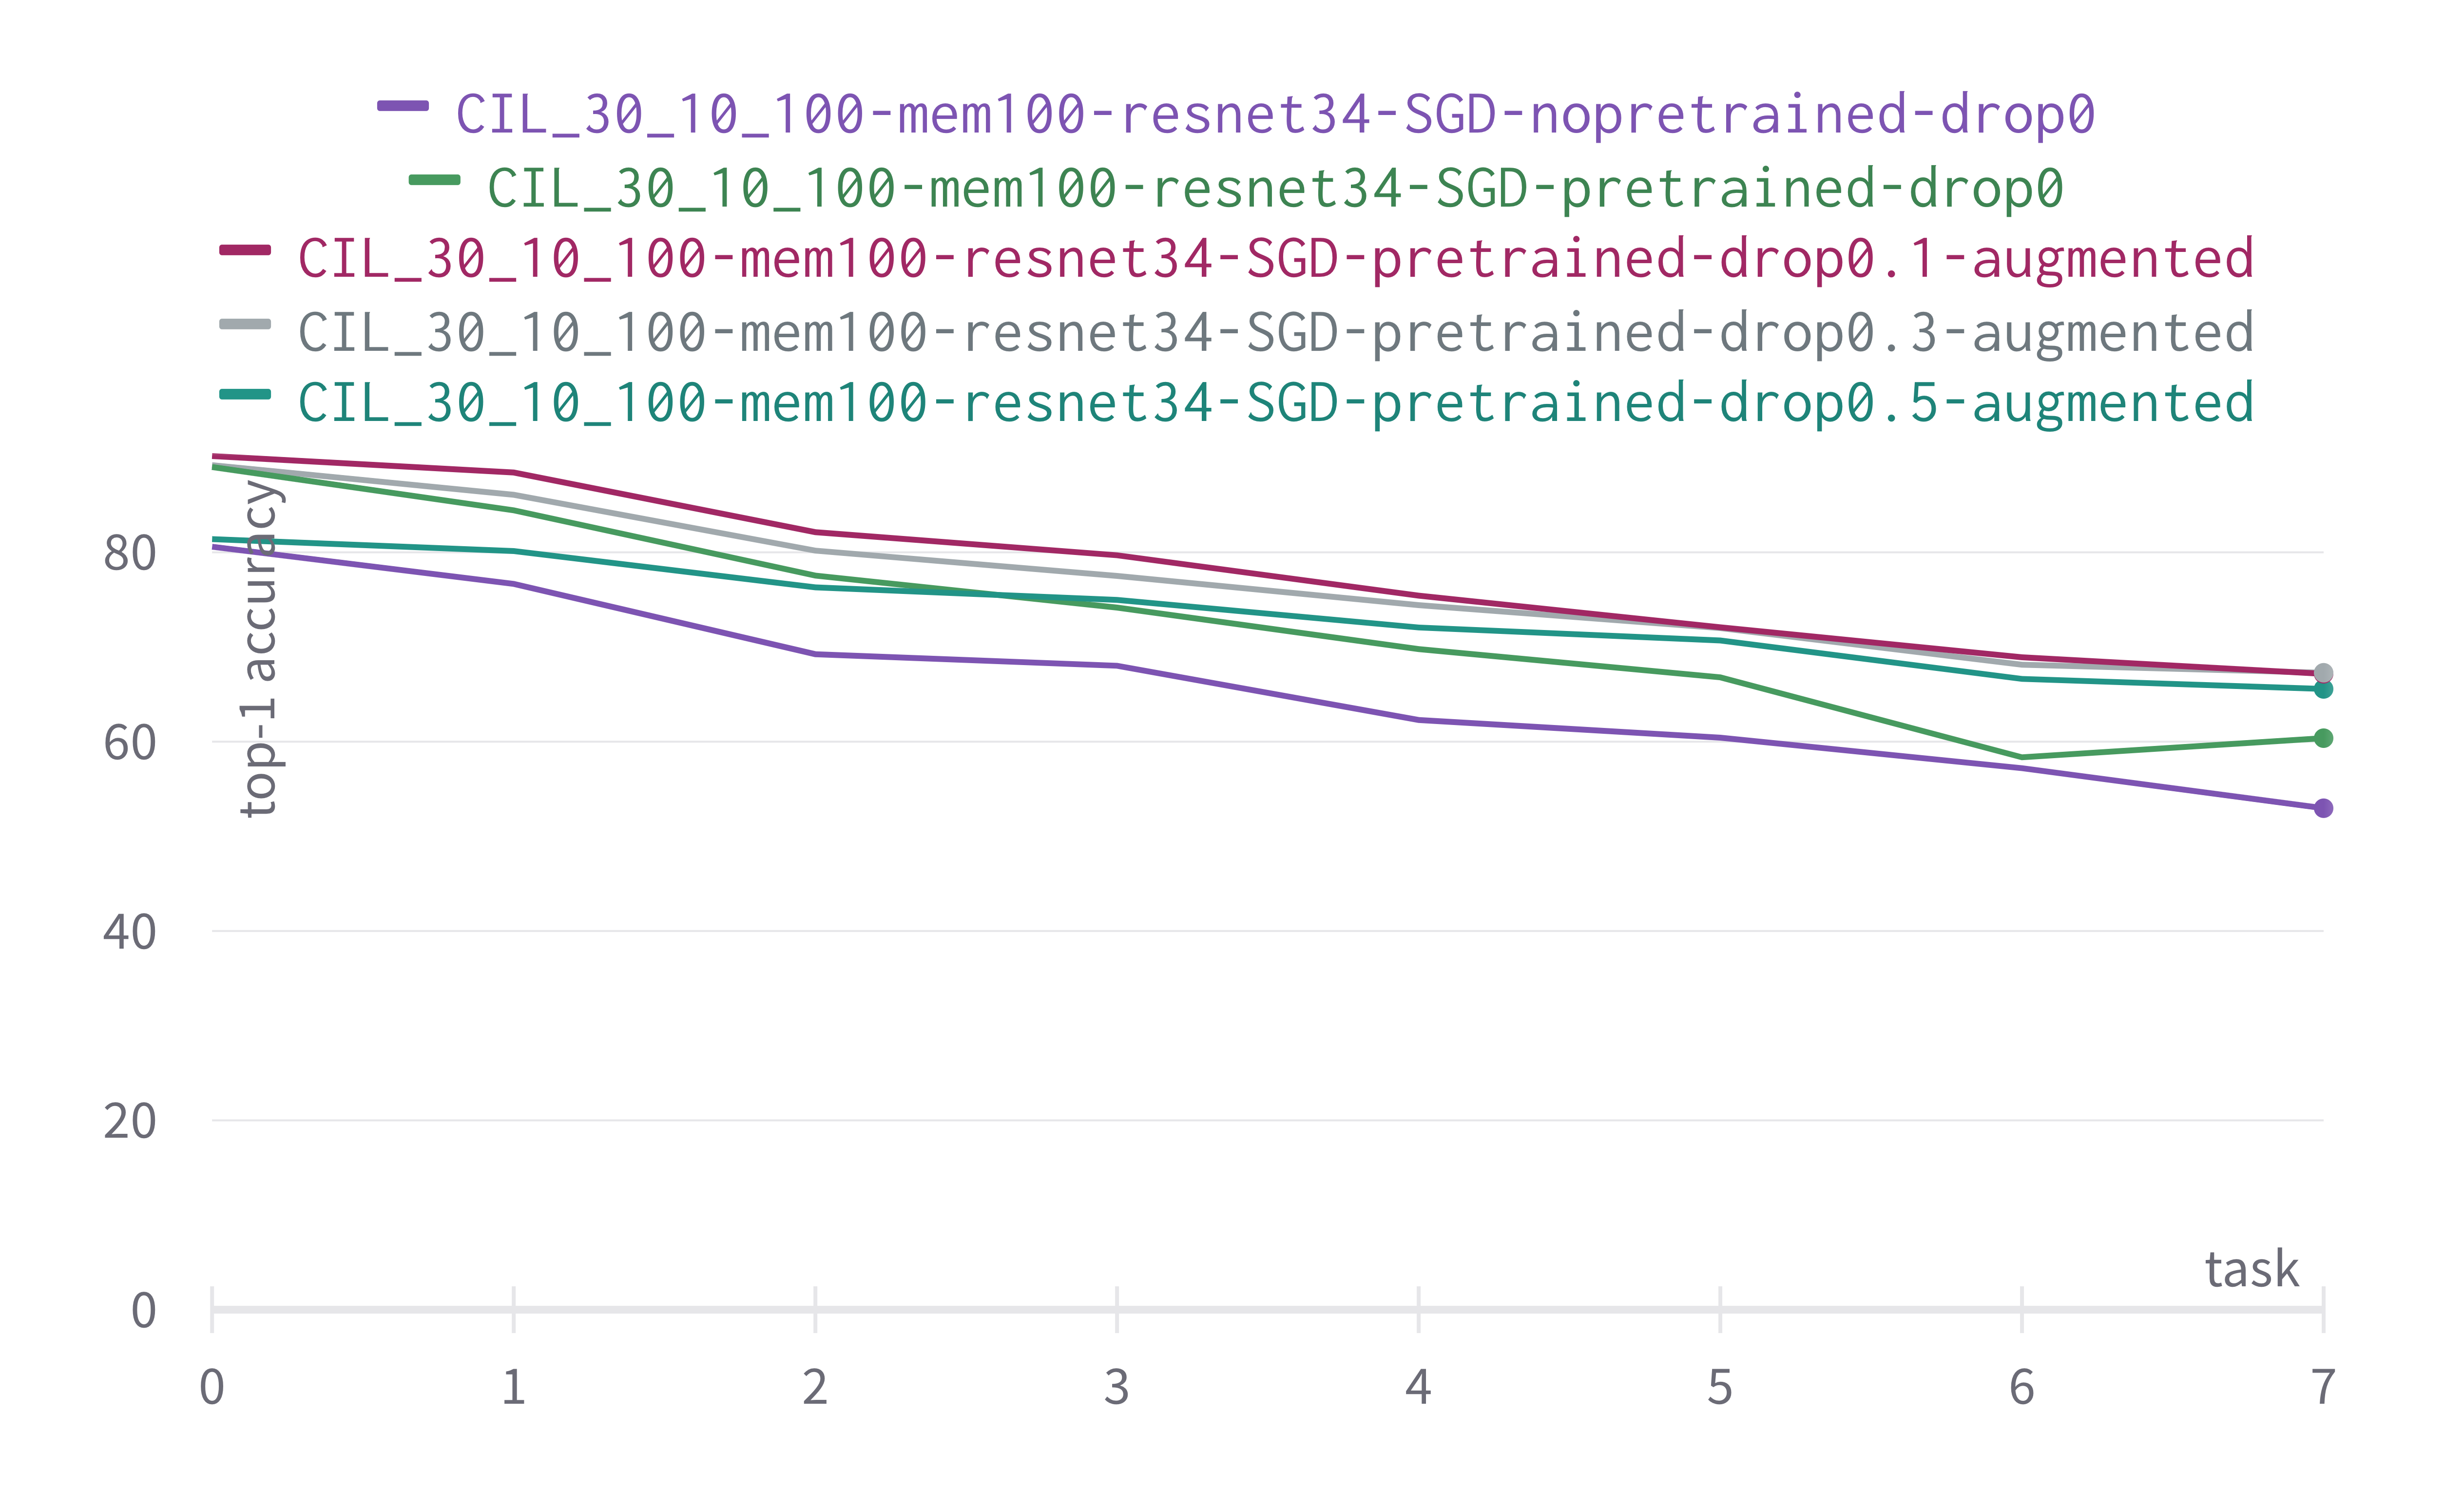
\includegraphics[width=0.80\textwidth]{images/exp/exp2-top1.png} }}%
    \qquad
	\subfloat[\centering Top-5 accuracy]{{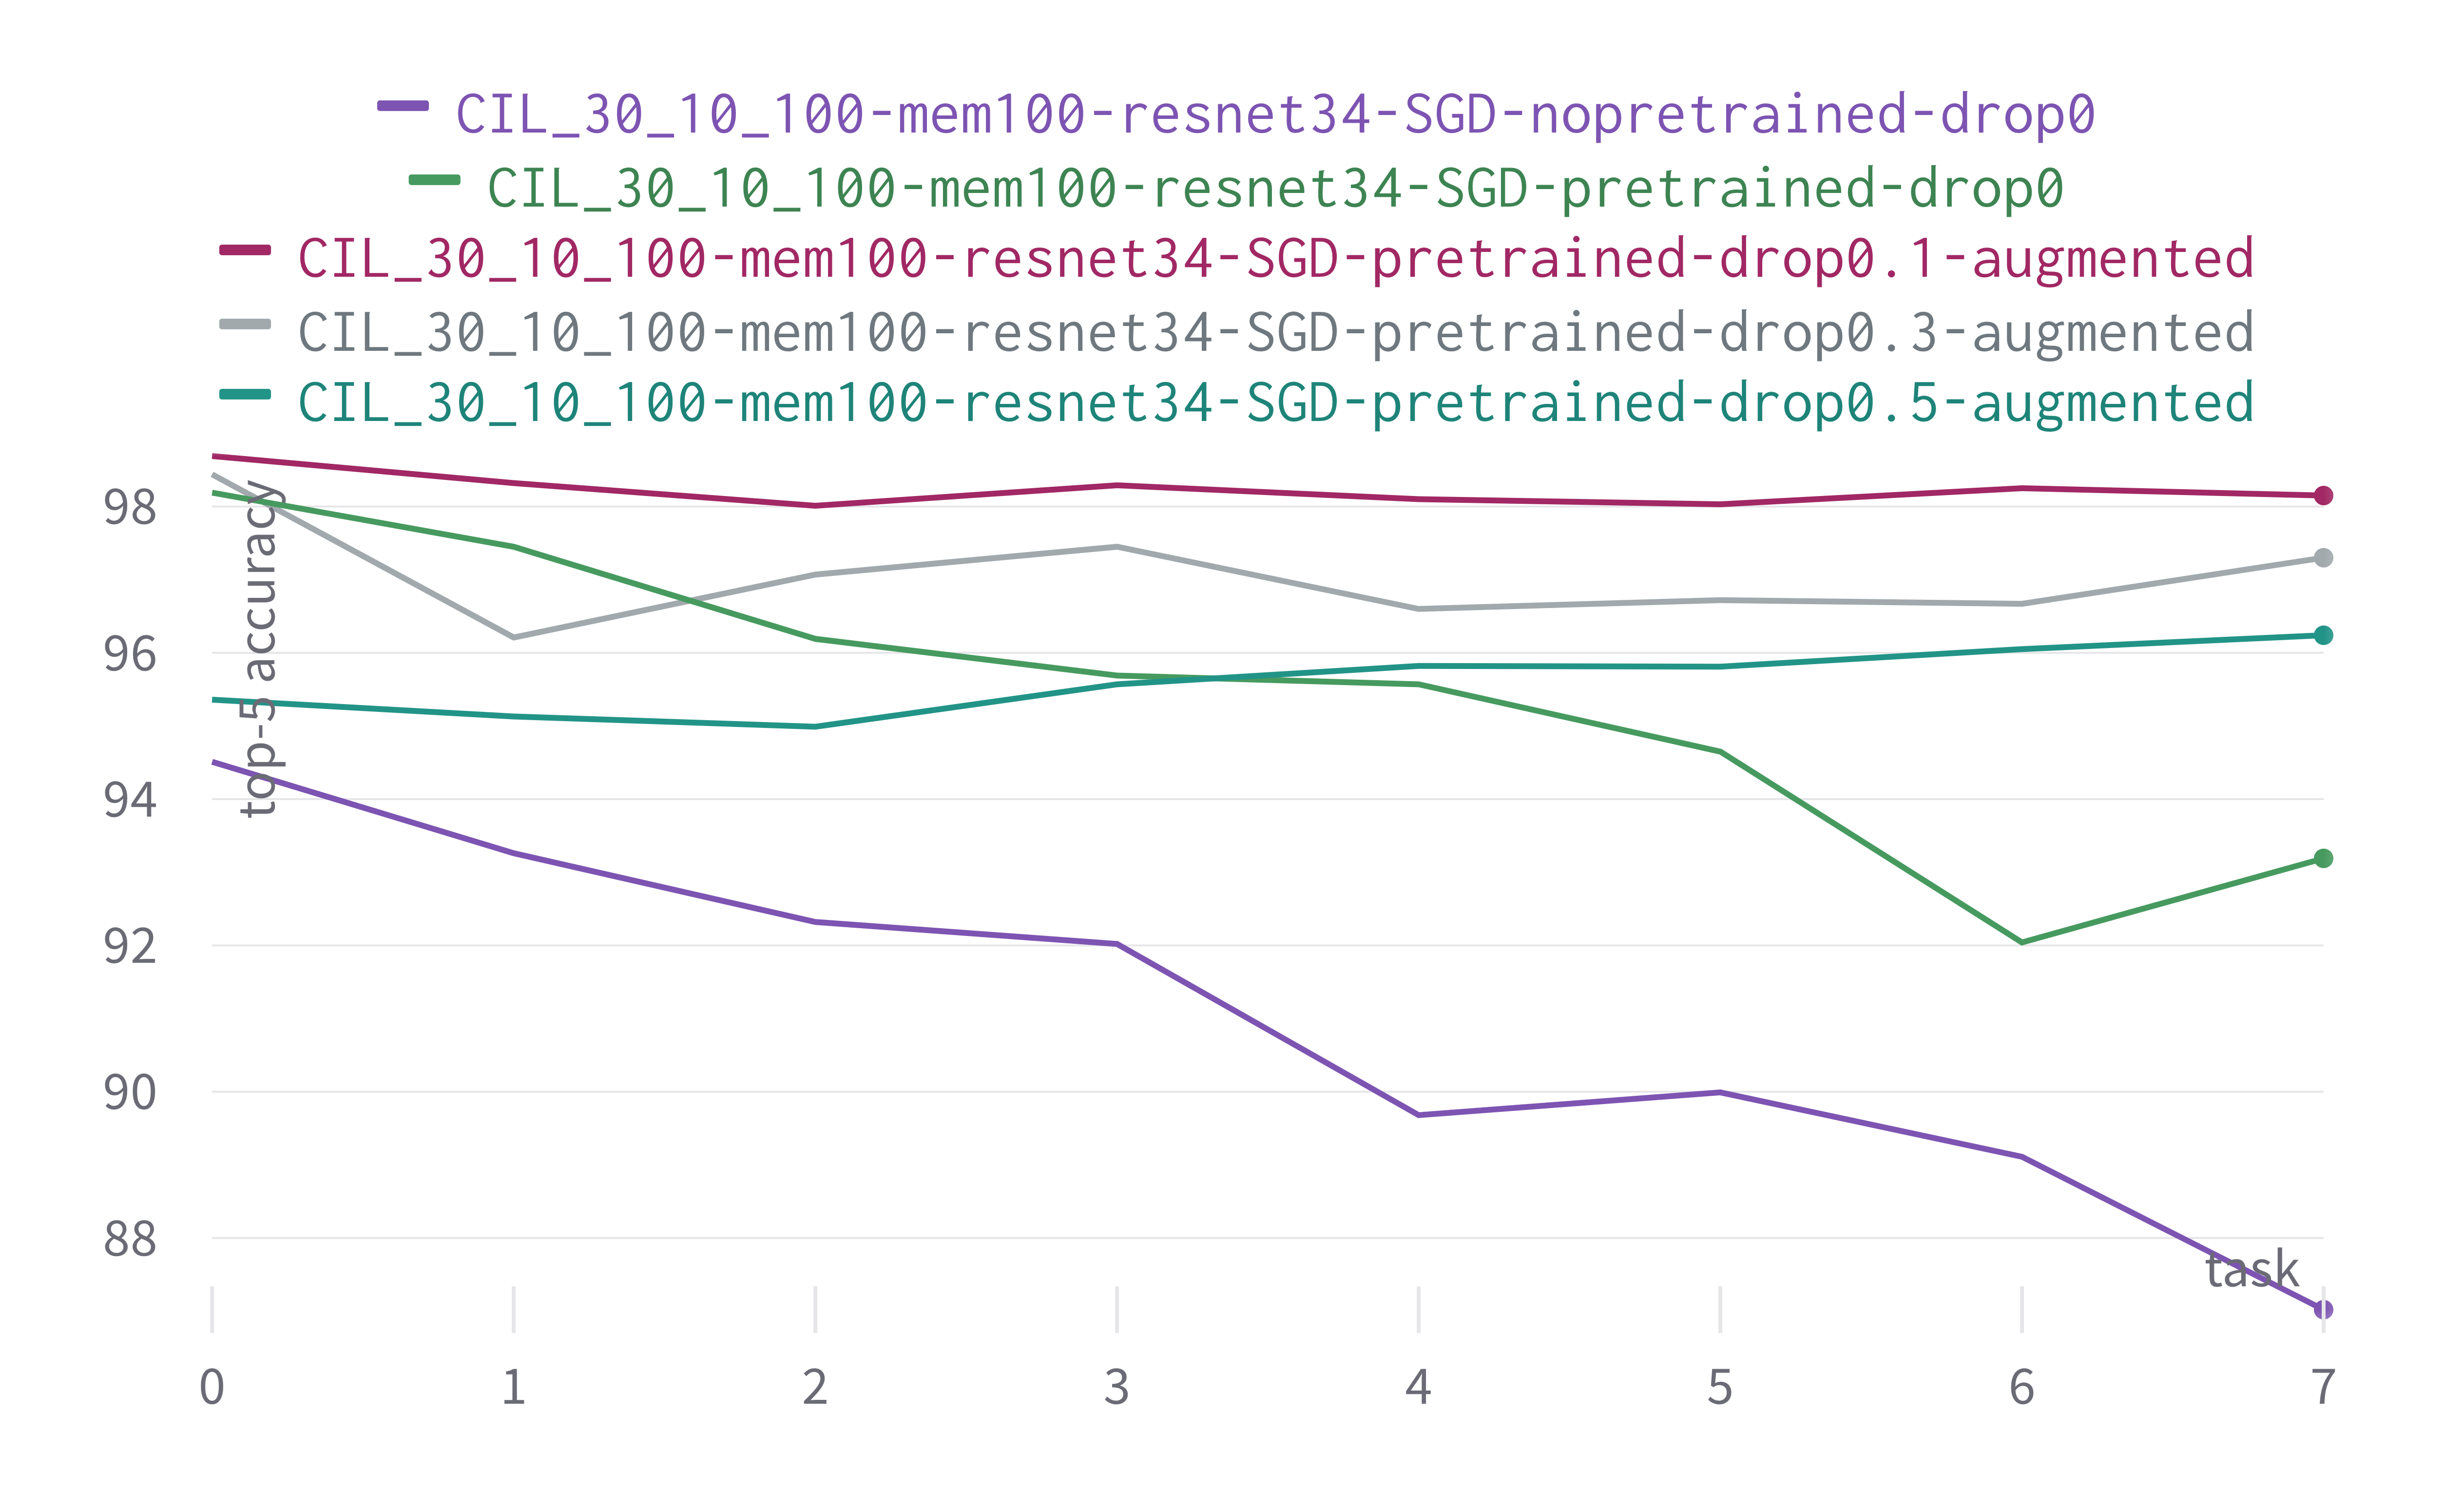
\includegraphics[width=0.80\textwidth]{images/exp/exp2-top5.png} }}%
	\caption{Top-1 and Top-5 accuracy of the regularized models using data augmentation.}%
	\label{fig:exp2}%
\end{figure}

\begin{figure}[H]
	\centering
	\subfloat[\centering Accuracy on the training set]{{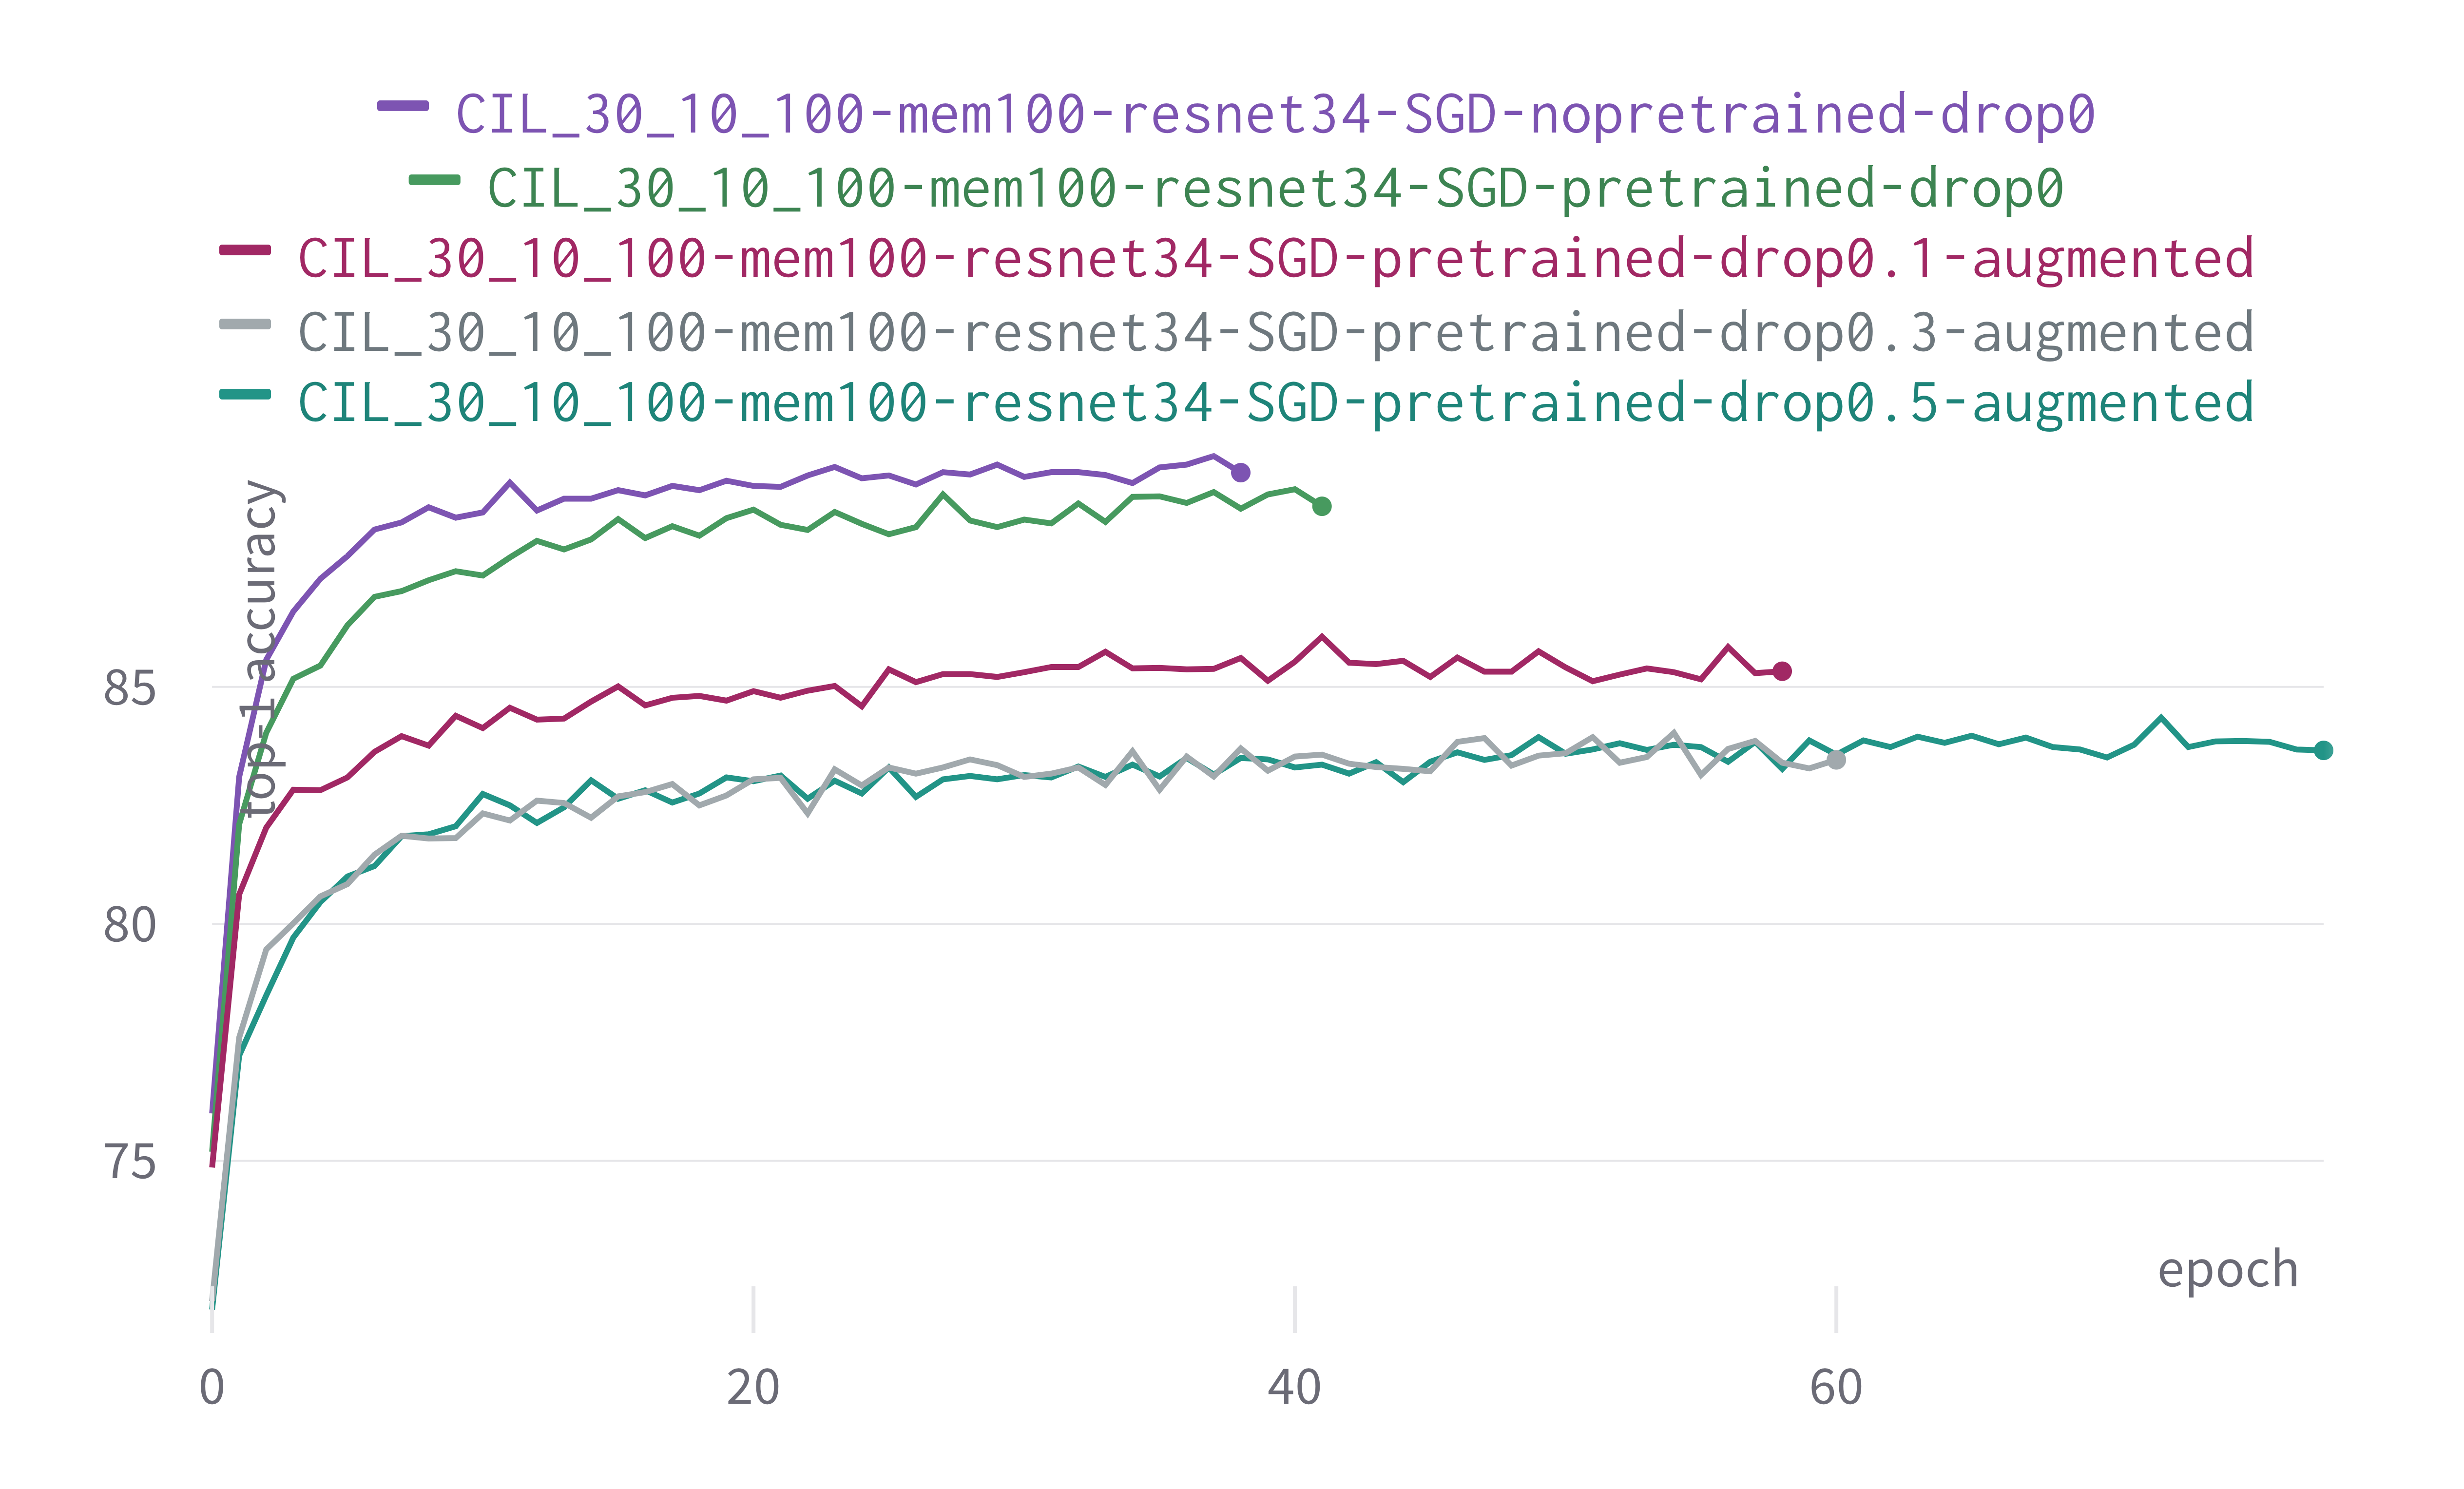
\includegraphics[width=0.80\textwidth]{images/exp/exp2-train.png} }}%
    \qquad
	\subfloat[\centering Accuracy on the validation set]{{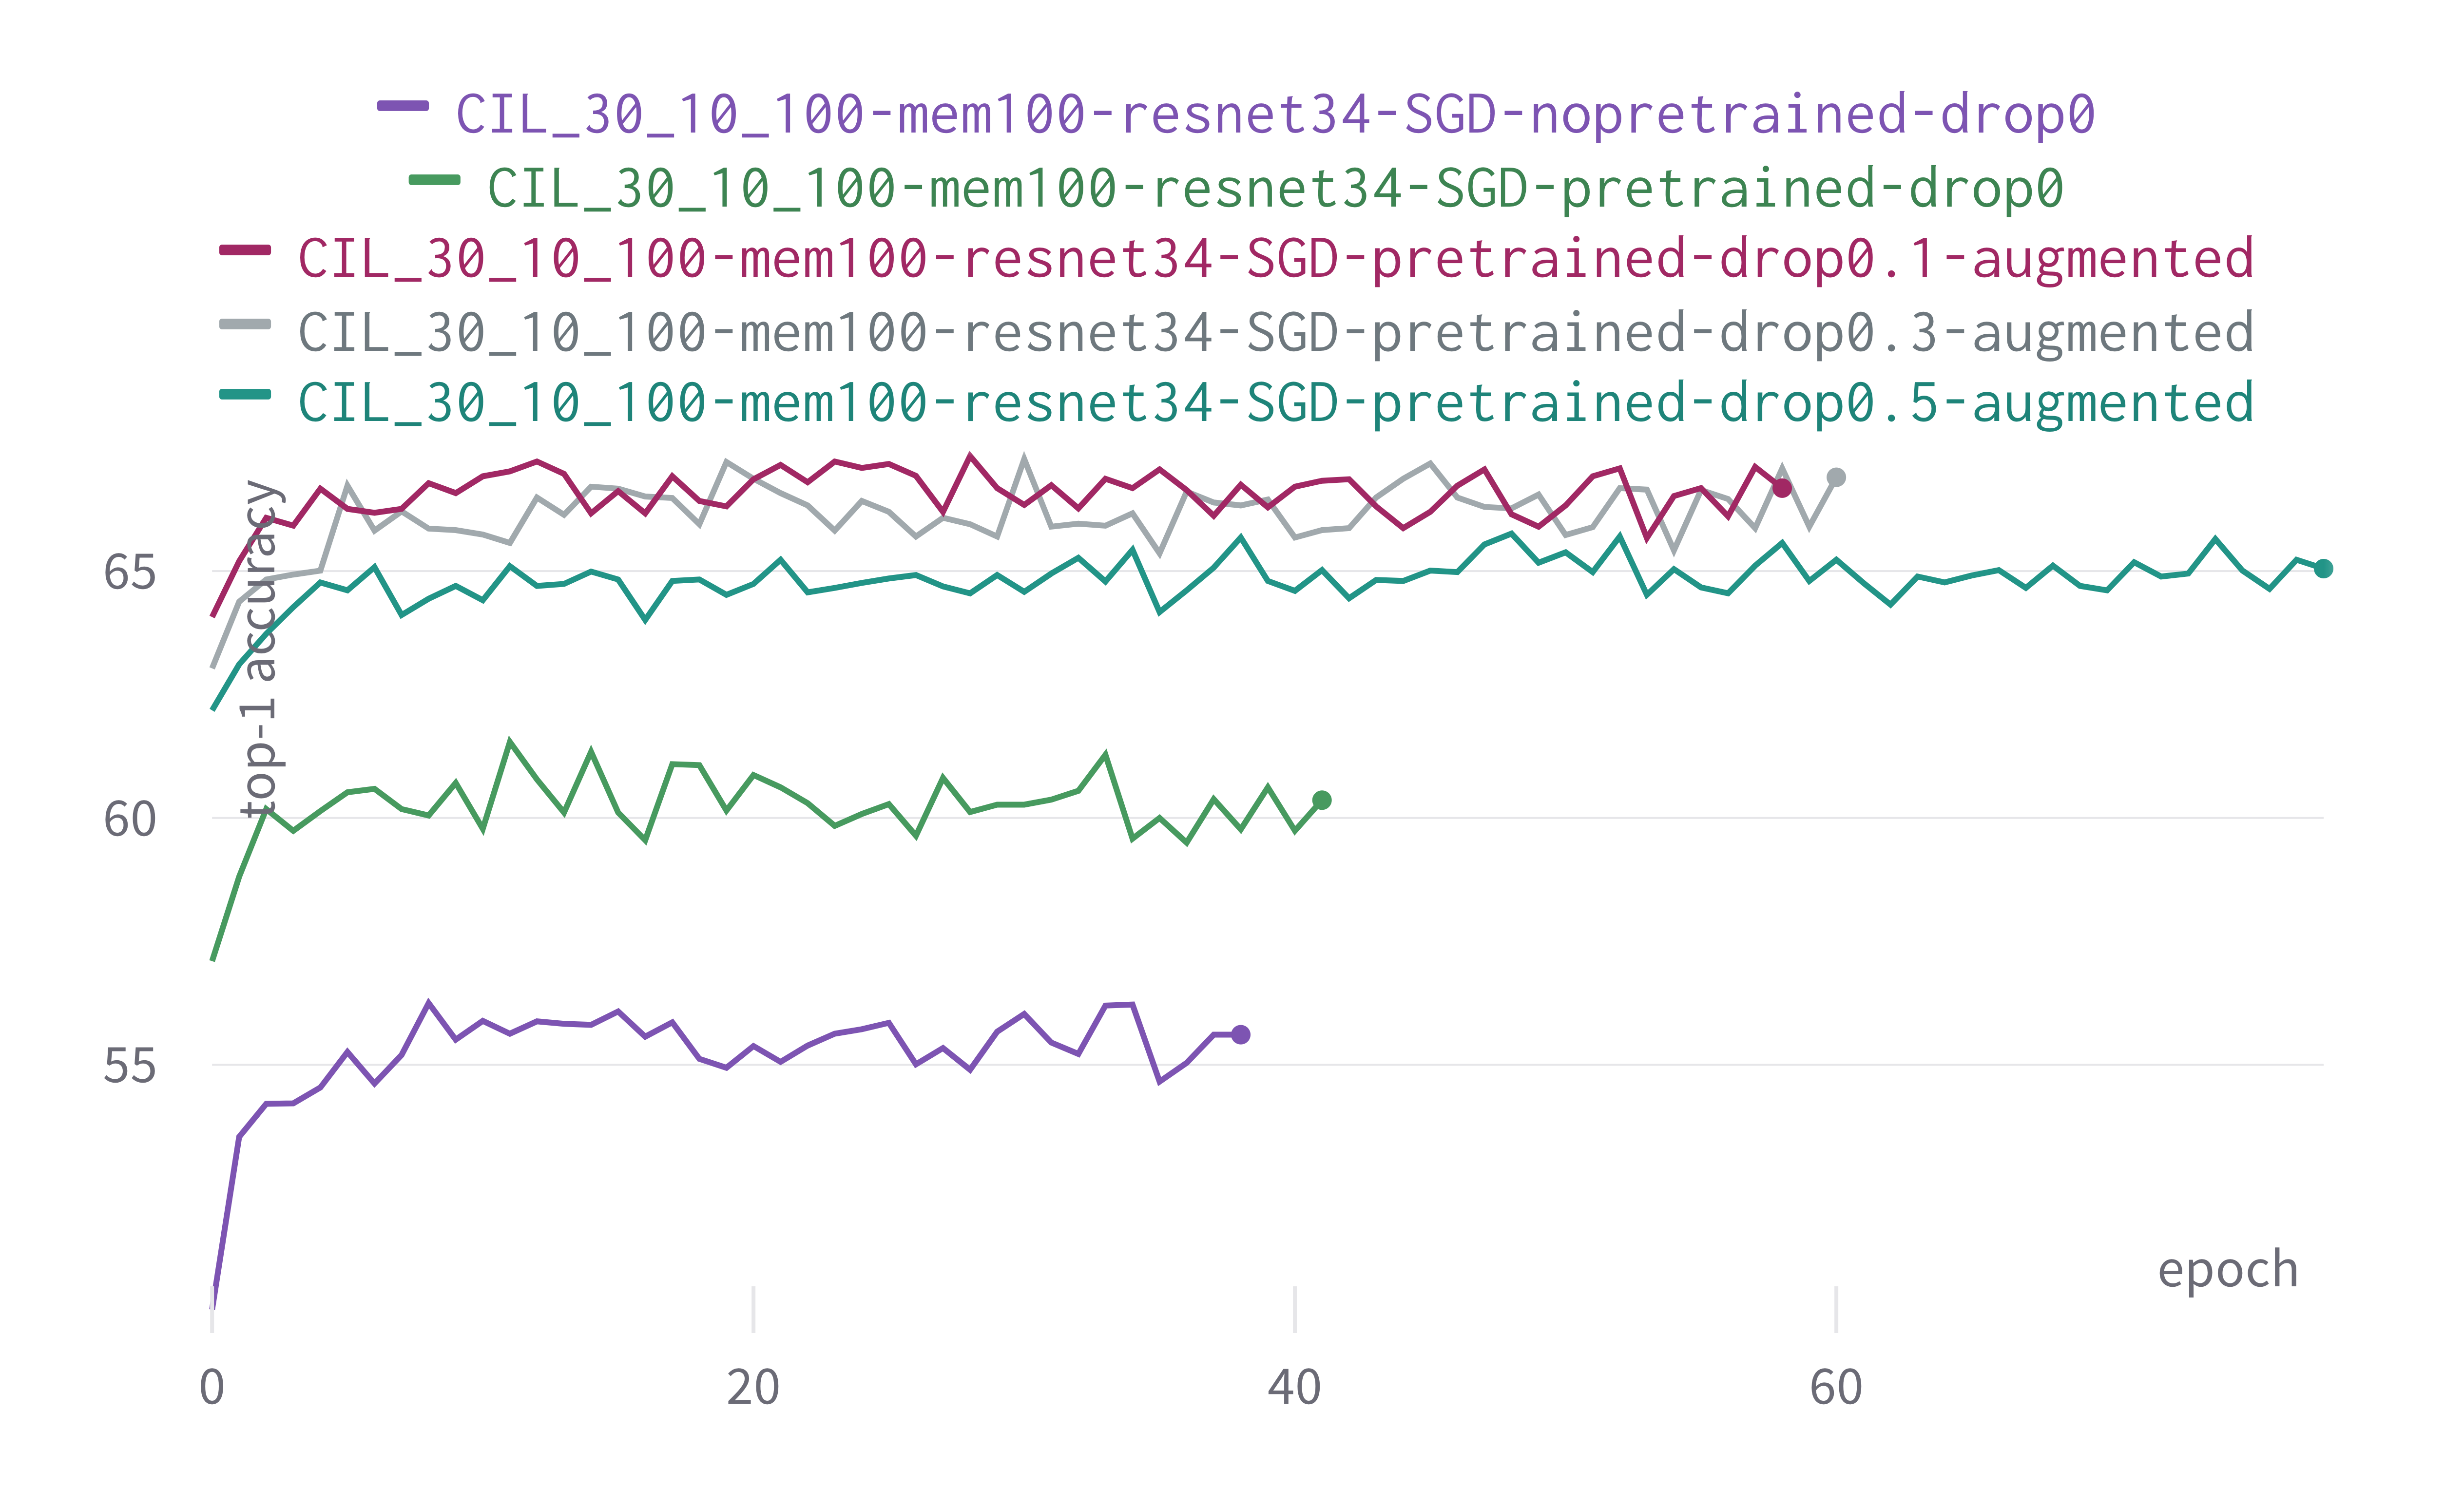
\includegraphics[width=0.80\textwidth]{images/exp/exp2-val.png} }}%
	\caption{Regularized models with data augmentation: comparison of the top-1 accuracy at each training epoch at task 7 between training and validation.}%
	\label{fig:exp2-train_val}%
\end{figure}

\newpage
\subsubsection{Type 1 baseline}
To compare the performance of the CIL model with a standard non-incremental learning setup, a baseline is trained using the same train/validation/test split of the CIL model. In particular, this experiment exploits the definition of 'type 1 baseline' described in \autoref{sec:method-baseline1}, i.e. it uses the DER algorithm and trains the model at task 0 with all 100 classes. Analogous to the CIL model, the baseline uses data augmentation, the SGD optimizer, a dropout layer before the FC layer and ResNet-34 pre-trained on ImageNet as backbone for the feature extract.

The performance comparison between the CIL models and the baselines is compared considering the top-1 accuracy on the test set. The results are shown in \autoref{table:baseline1}. As we can see, the best CIL model performs better than the best baseline, which is the opposite of what one might expect. However, as we can see from \autoref{table:baseline1-params}, this is due to the difference in the number of parameters described in \autoref{sec:method-baseline1}. For this reason, in the section section the CIL models are compared using a different type of baseline.

\begin{table}[H]
    \centering
    \centerline{
    \begin{tabular}{c|c|c|c}
        \hline
        \textbf{Model} &
        \textbf{Dropout} &
        \textbf{Top-1} & 
        \textbf{Top-5} \\
        \textbf{name} &
        \textbf{rate} &
        \textbf{acc. (\%)} & 
        \textbf{acc. (\%)} \\
        \hline
\hline
SGD-pretrained-drop0.1-augmented&0.1&67.17\\
SGD-pretrained-drop0.3-augmented&0.3&\textbf{67.28}\\
SGD-pretrained-drop0.5-augmented&0.5&65.57\\
\hline
BASELINE\_1-pretrained-drop0.1-augmented&0.1&63.04\\
BASELINE\_1-pretrained-drop0.3-augmented&0.3&61.15\\
BASELINE\_1-pretrained-drop0.5-augmented&0.5&57.14\\
\hline 
    \end{tabular}}
    \caption{Performance comparison between the CIL model and the type 1 baseline. Top-1 accuracy at task 7 (CIL model) and task 0 (baseline).}
    \label{table:baseline1}
\end{table}

\begin{table}[H]
    \centering
    \centerline{
    \begin{tabular}{c|c}
        \hline
        \textbf{Model} &
        \textbf{\#Params} \\
        \textbf{name} &
        \textbf{(M)} \\
        \hline
\hline
SGD-pretrained-drop0.1-augmented&170\\
SGD-pretrained-drop0.3-augmented&170\\
SGD-pretrained-drop0.5-augmented&170\\
\hline
BASELINE\_1-pretrained-drop0.1-augmented&21\\
BASELINE\_1-pretrained-drop0.3-augmented&21\\
BASELINE\_1-pretrained-drop0.5-augmented&21\\
\hline 
    \end{tabular}}
    \caption{Number of model parameters between the CIL model and the typ 1 baseline. Number of parameters at task 7 (CIL model) and task 0 (baseline).}
    \label{table:baseline1-params}
\end{table}

\subsubsection{Top-100 Classes}
\label{sec:cil-top100}
In order to assess the extent to which those classes with few examples contribute to performance deterioration, the next experiments are carried out by considering only the top-100 classes, i.e. those with the largest number of examples (see the left-hand side of the distribution in \autoref{fig:logodet-dist}). This is useful to be aware of how much the model is limited in performance by the dataset.

Considering the regularized models and data augmentation, models trained on 100 randomly sampled classes and those trained on the top-100 classes are compared in \autoref{fig:exp3} and \autoref{table:exp3}. As we can see, even if the top-5 accuracy does not change between the two cases, considering the top-1 accuracy there is a drastic improvement in performance. This is a clear sign that classes with few examples deteriorate performance a lot.

\begin{table}[H]
    \centering
    \centerline{
    \begin{tabular}{c|c|c|c|c}
        \hline
        \textbf{Model} &
        \textbf{Dropout} &
        \textbf{Sampling} &
        \textbf{Top-1} & 
        \textbf{Top-5} \\
        \textbf{name} &
        \textbf{rate} &
        \textbf{method} &
        \textbf{acc. (\%)} & 
        \textbf{acc. (\%)} \\
        \hline
        \hline
drop0.1-augmented&0.1&random&	67.17&98.15\\
drop0.3-augmented&0.3&random&67.28&	97.3\\
drop0.5-augmented&0.5&random&65.57&	96.24\\
\hline
drop0.1-augmented-onlytop&0.1&top-100&\textbf{89.1}&\textbf{96.59}\\
drop0.3-augmented-onlytop&0.3&top-100&88.14&96.39\\
drop0.5-augmented-onlytop&0.5&top-100&87.6&95.92\\
        \hline
    \end{tabular}}
    \caption{Comparison of models trained on 100 randomly sampled classed and top-100 classes. Top-1 accuracy at task 7.}
    \label{table:exp3}
\end{table}
\newpage
\begin{figure}[H]
	\centering
	\subfloat[\centering Top-1 accuracy]{{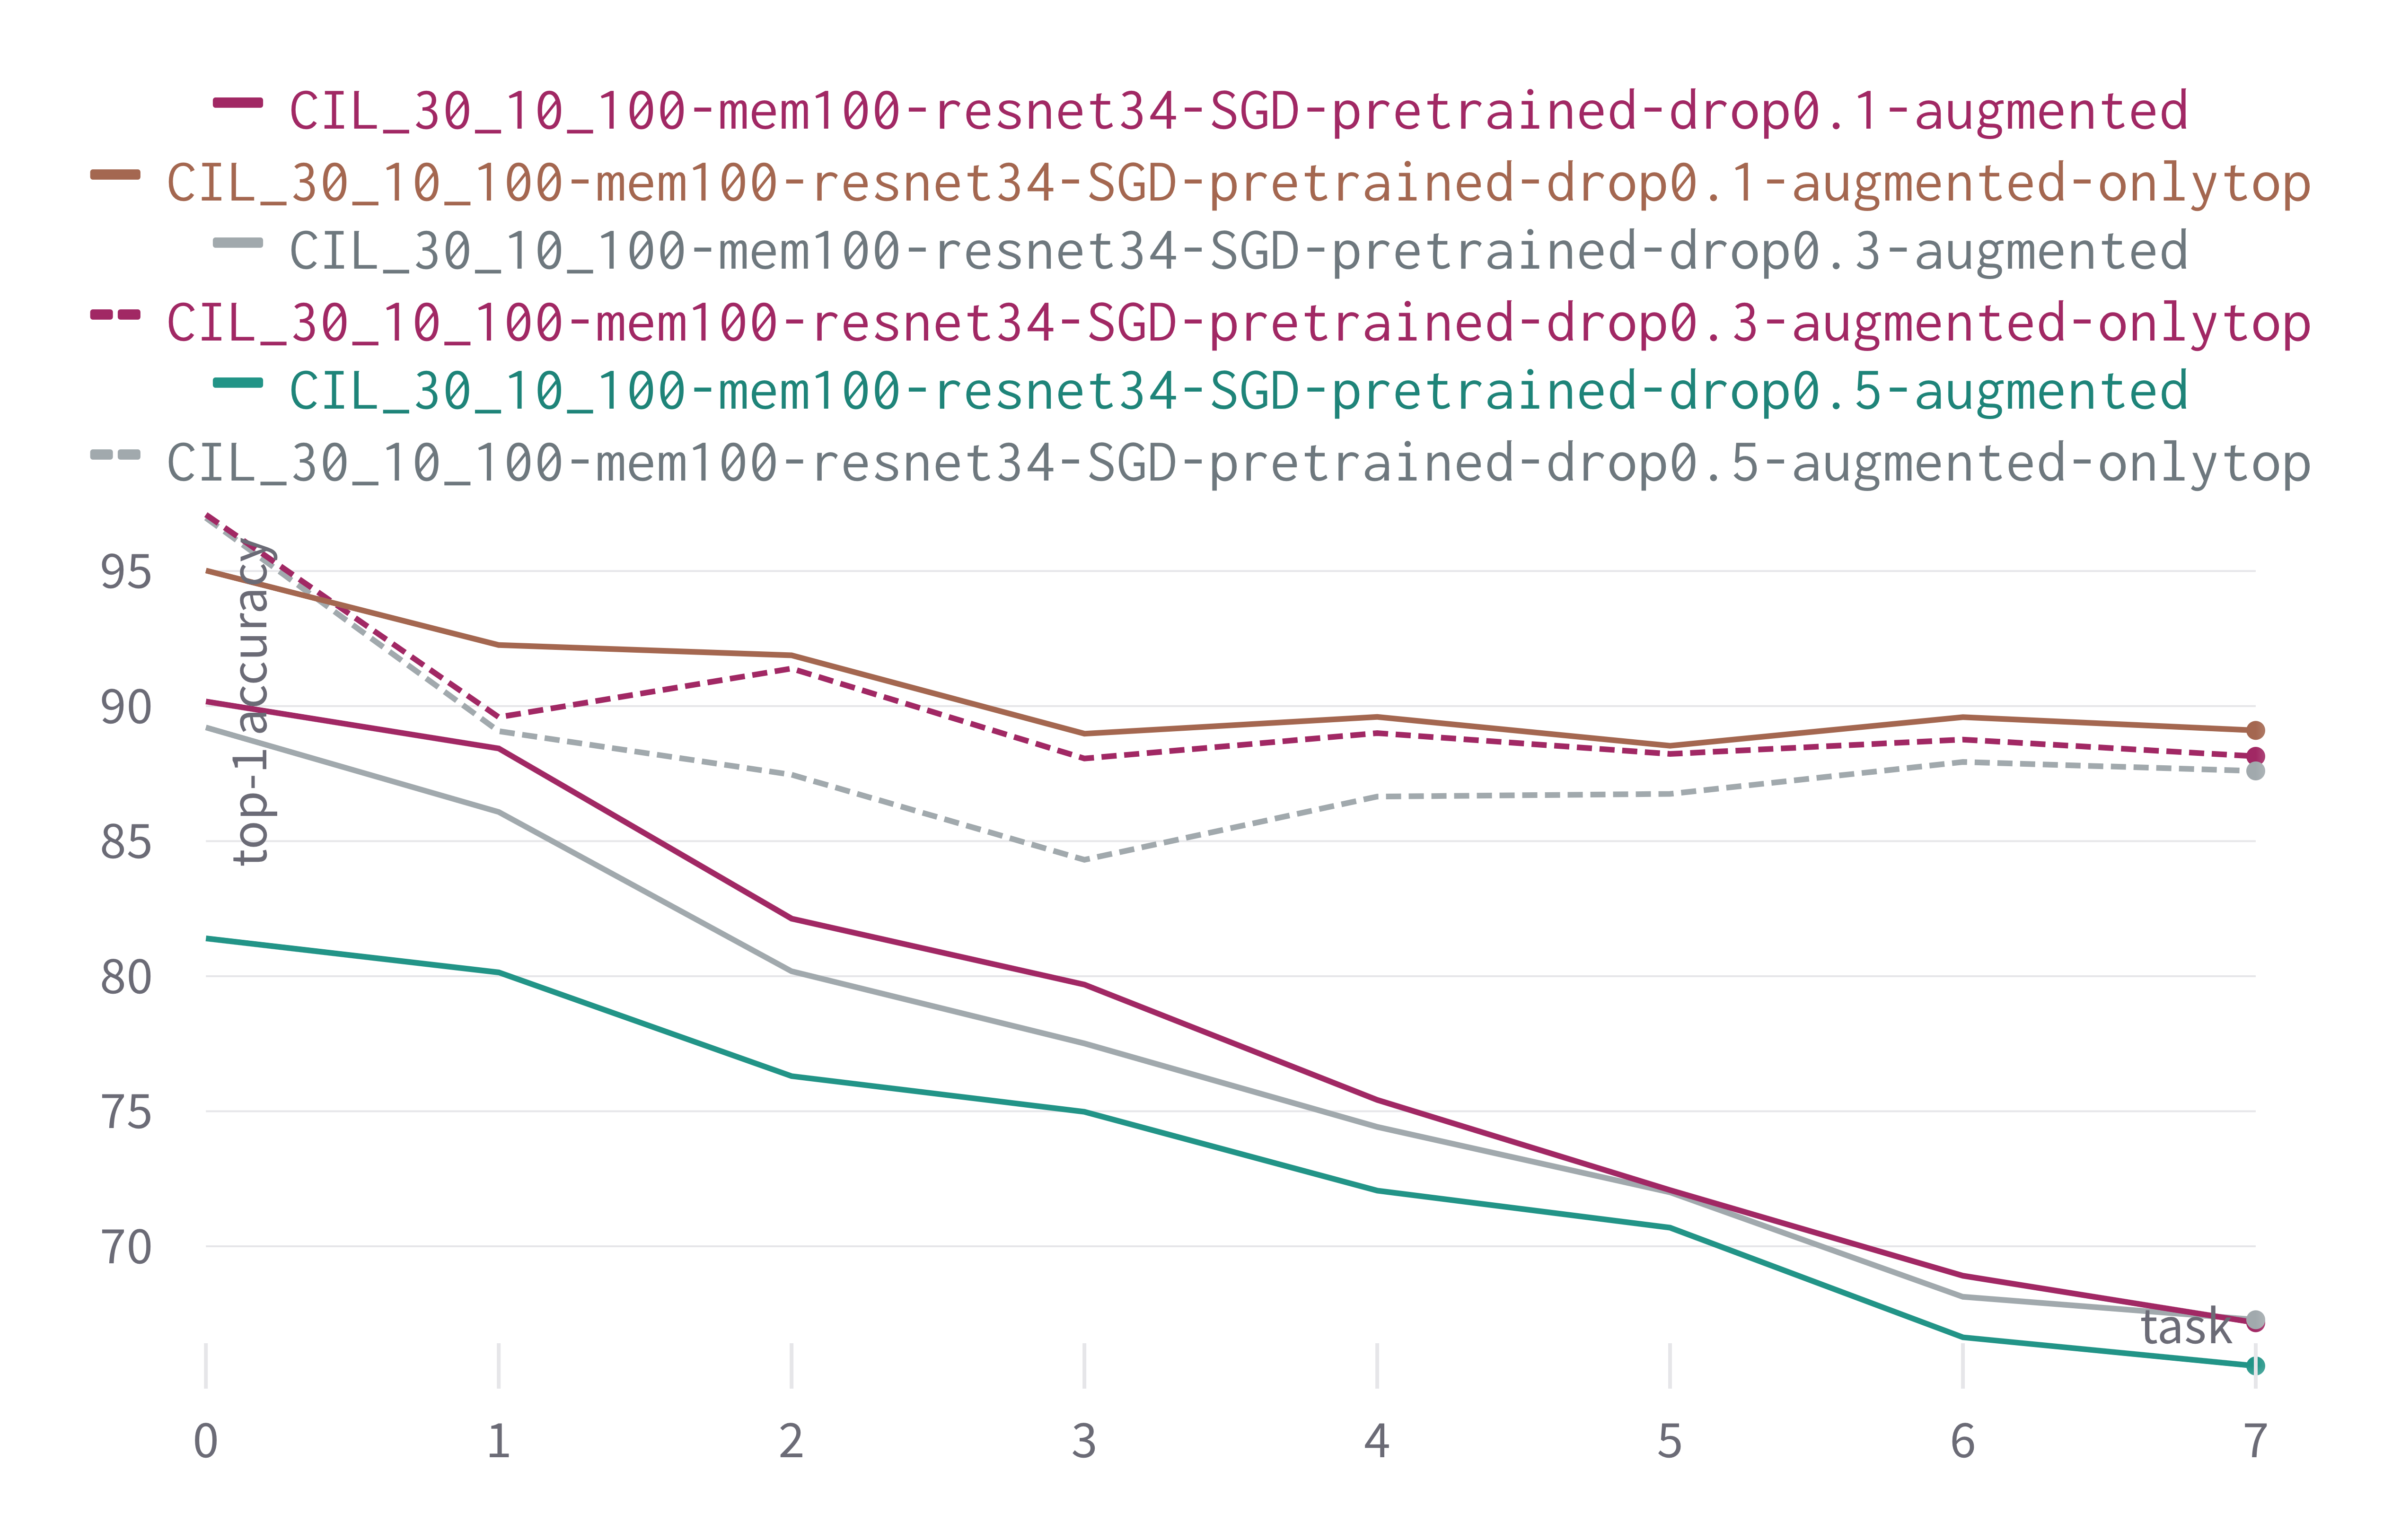
\includegraphics[width=0.80\textwidth]{images/exp/exp3-top1.png} }}%
    \qquad
	\subfloat[\centering Top-5 accuracy]{{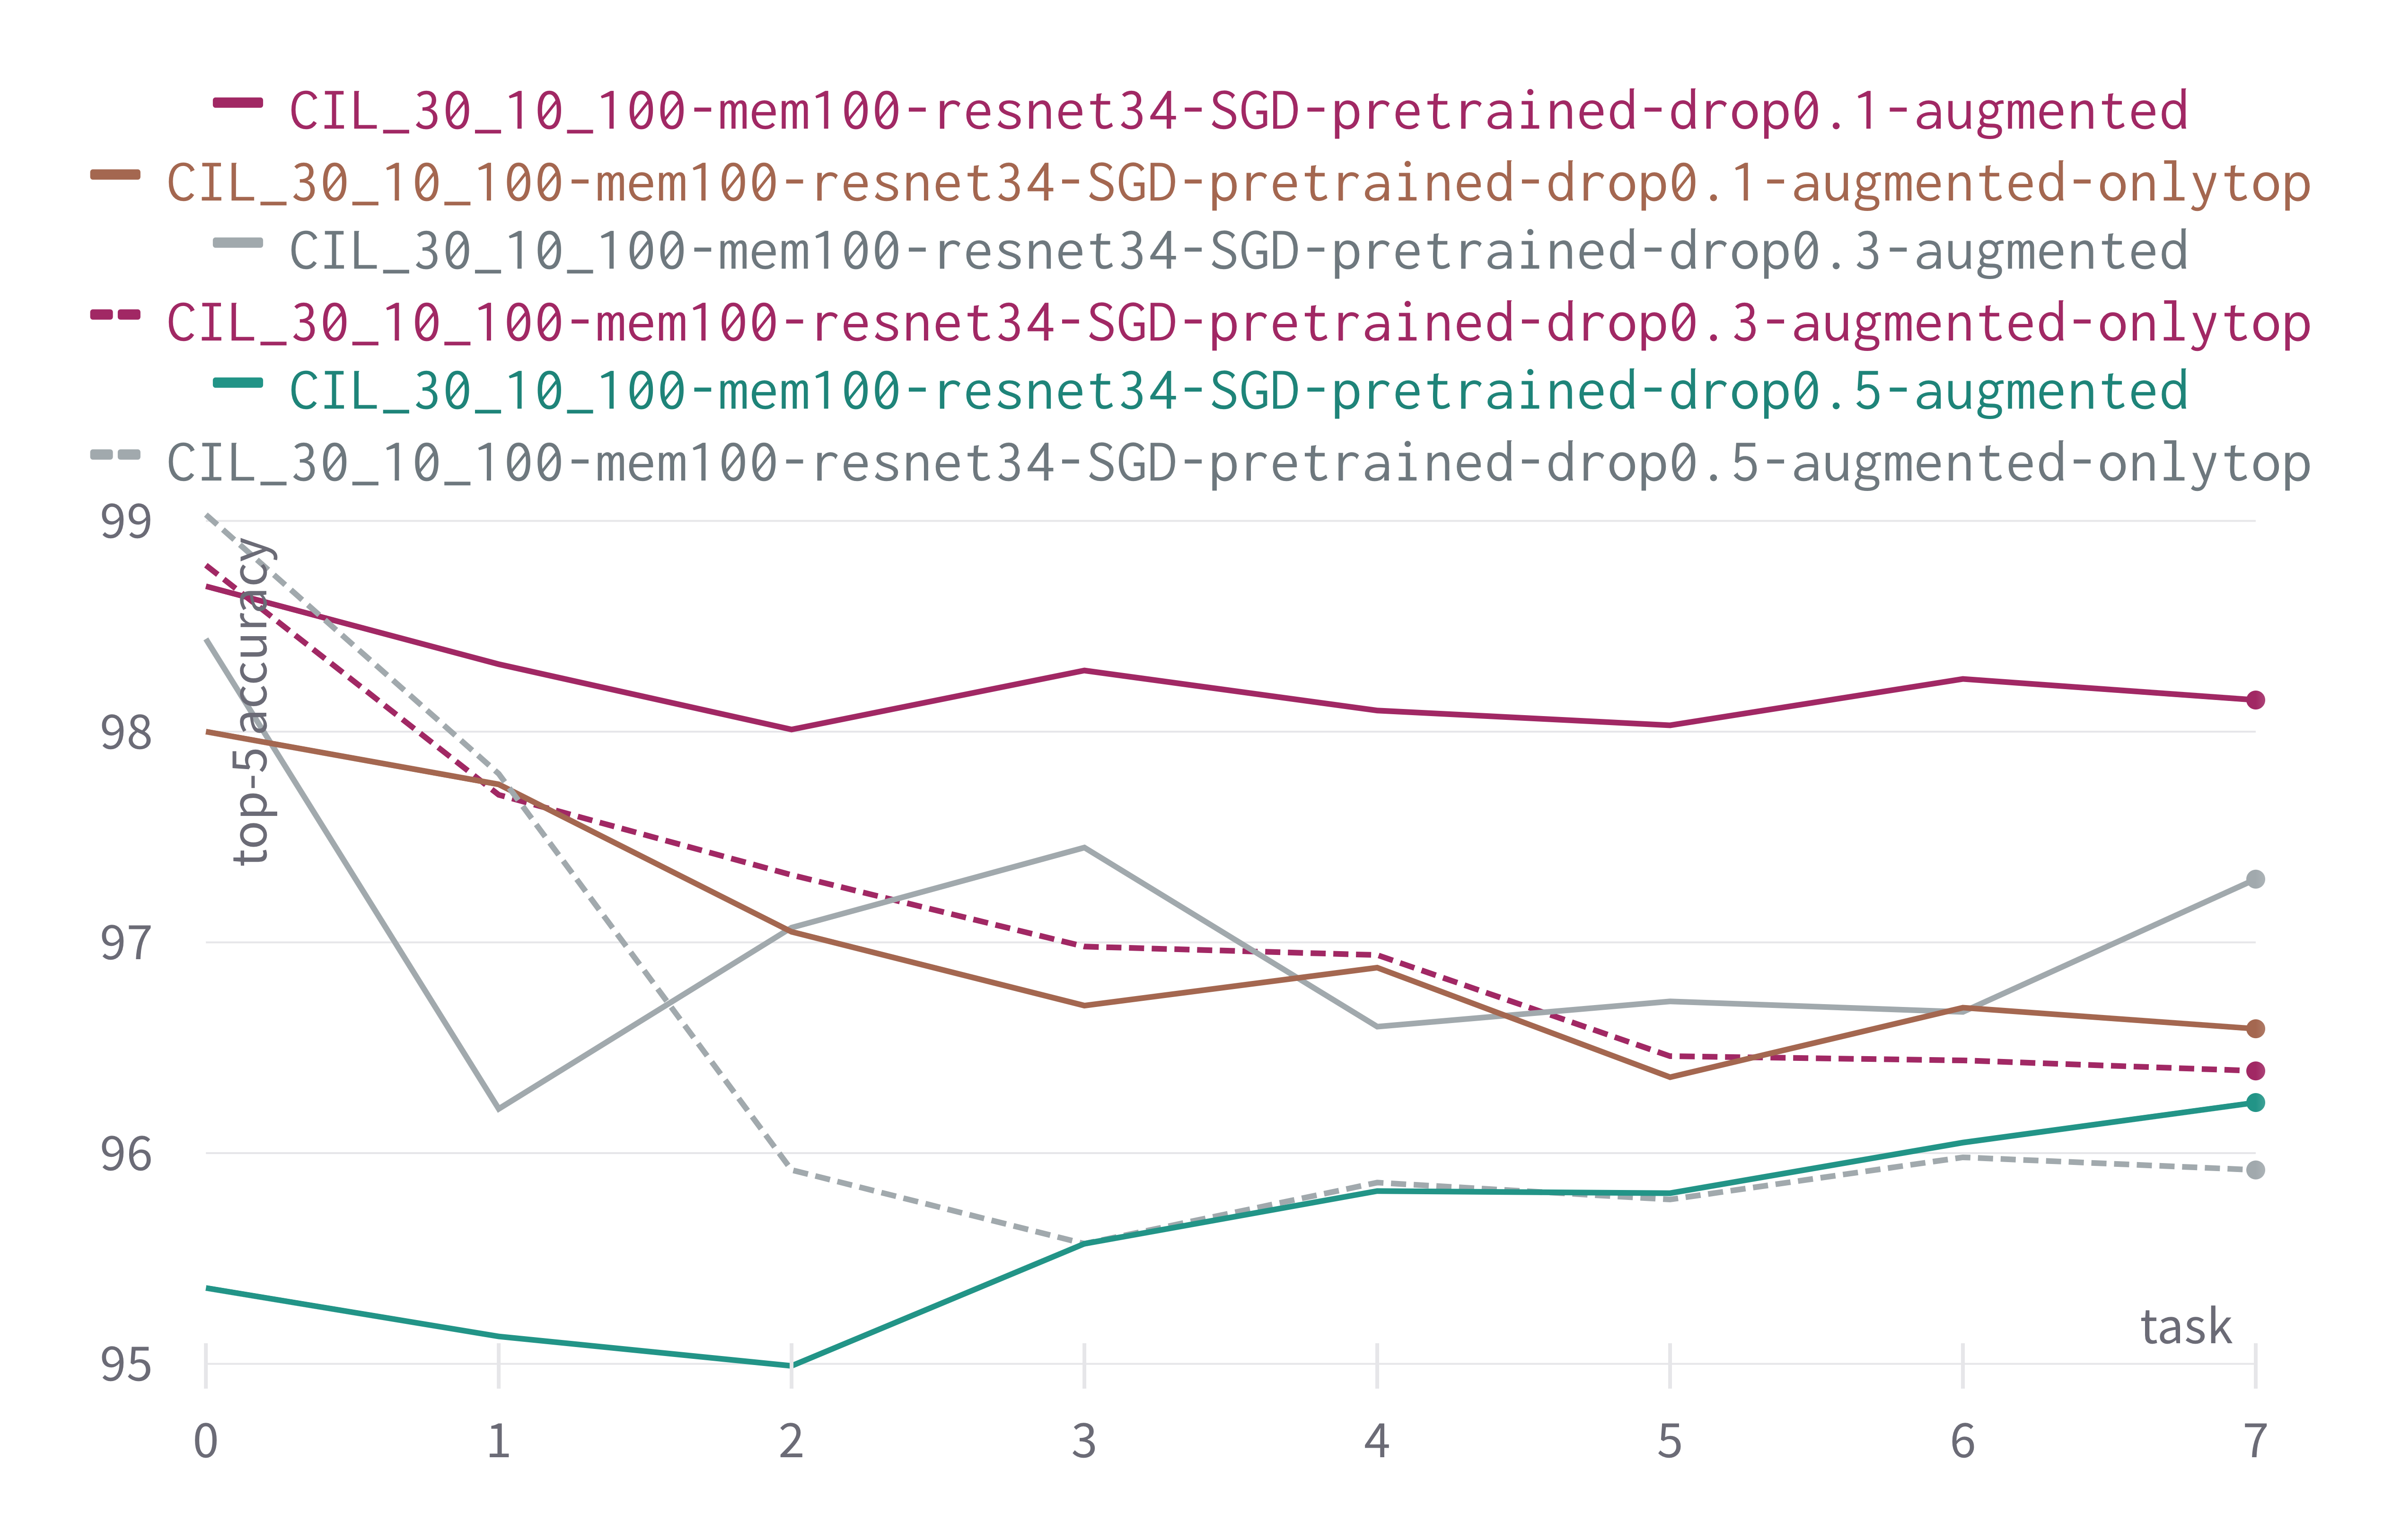
\includegraphics[width=0.80\textwidth]{images/exp/exp3-top5.png} }}%
	\caption{Comparison of models trained on 100 randomly sampled classed and top-100 classes.}%
	\label{fig:exp3}%
\end{figure}

\newpage
\subsubsection{Introduction of Adam optimizer}
The next experiments aim to compare the SGD (see \autoref{sec:sgd_opt}) and Adam (see \autoref{sec:adam_opt}) optimizers. Considering the regularized models, data augmentation and the top-100 classes, the result of this comparison is shown in \autoref{fig:exp4} and \autoref{table:exp4}.


As we can see from the results shown in \autoref{table:exp4}, the top-1 accuracy at task 7 improves by more than 6\% using the Adam as the optimization algorithm. 
In addition to the performance aspect, the training history in \autoref{fig:exp4-train_val} shows that Adam leads to faster convergence. In fact the models trained with this algorithm achieve the highest value of top-1 accuracy on the validation set after only a few training epochs.

\begin{table}[H]
    \centering
    \centerline{
    \begin{tabular}{c|c|c|c|c}
        \hline
        \textbf{Model} &
        \textbf{Dropout} &
        \textbf{Optimizer} &
        \textbf{Top-1} & 
        \textbf{Top-5} \\
        \textbf{name} &
        \textbf{rate} &
        \textbf{method} &
        \textbf{acc. (\%)} & 
        \textbf{acc. (\%)} \\
        \hline
        \hline
SGD-drop0.1-augmented-onlytop&0.1&SGD&89.1&96.59\\
SGD-drop0.3-augmented-onlytop&0.3&SGD&88.14&96.39\\
SGD-drop0.5-augmented-onlytop&0.5&SGD&87.6&95.92\\
\hline
adam-drop0.1-augmented-onlytop&0.1&Adam&92.15&97.92\\
adam-drop0.3-augmented-onlytop&0.3&Adam&91.55&97.75\\
adam-drop0.5-augmented-onlytop&0.5&Adam&\textbf{95.04}&\textbf{98.4}\\
        \hline
    \end{tabular}}
    \caption{Comparison of models trained using SGD and Adam. Top-1 accuracy at task 7.}
    \label{table:exp4}
\end{table}

\newpage

\begin{figure}[H]
	\centering
	\subfloat[\centering Top-1 accuracy]{{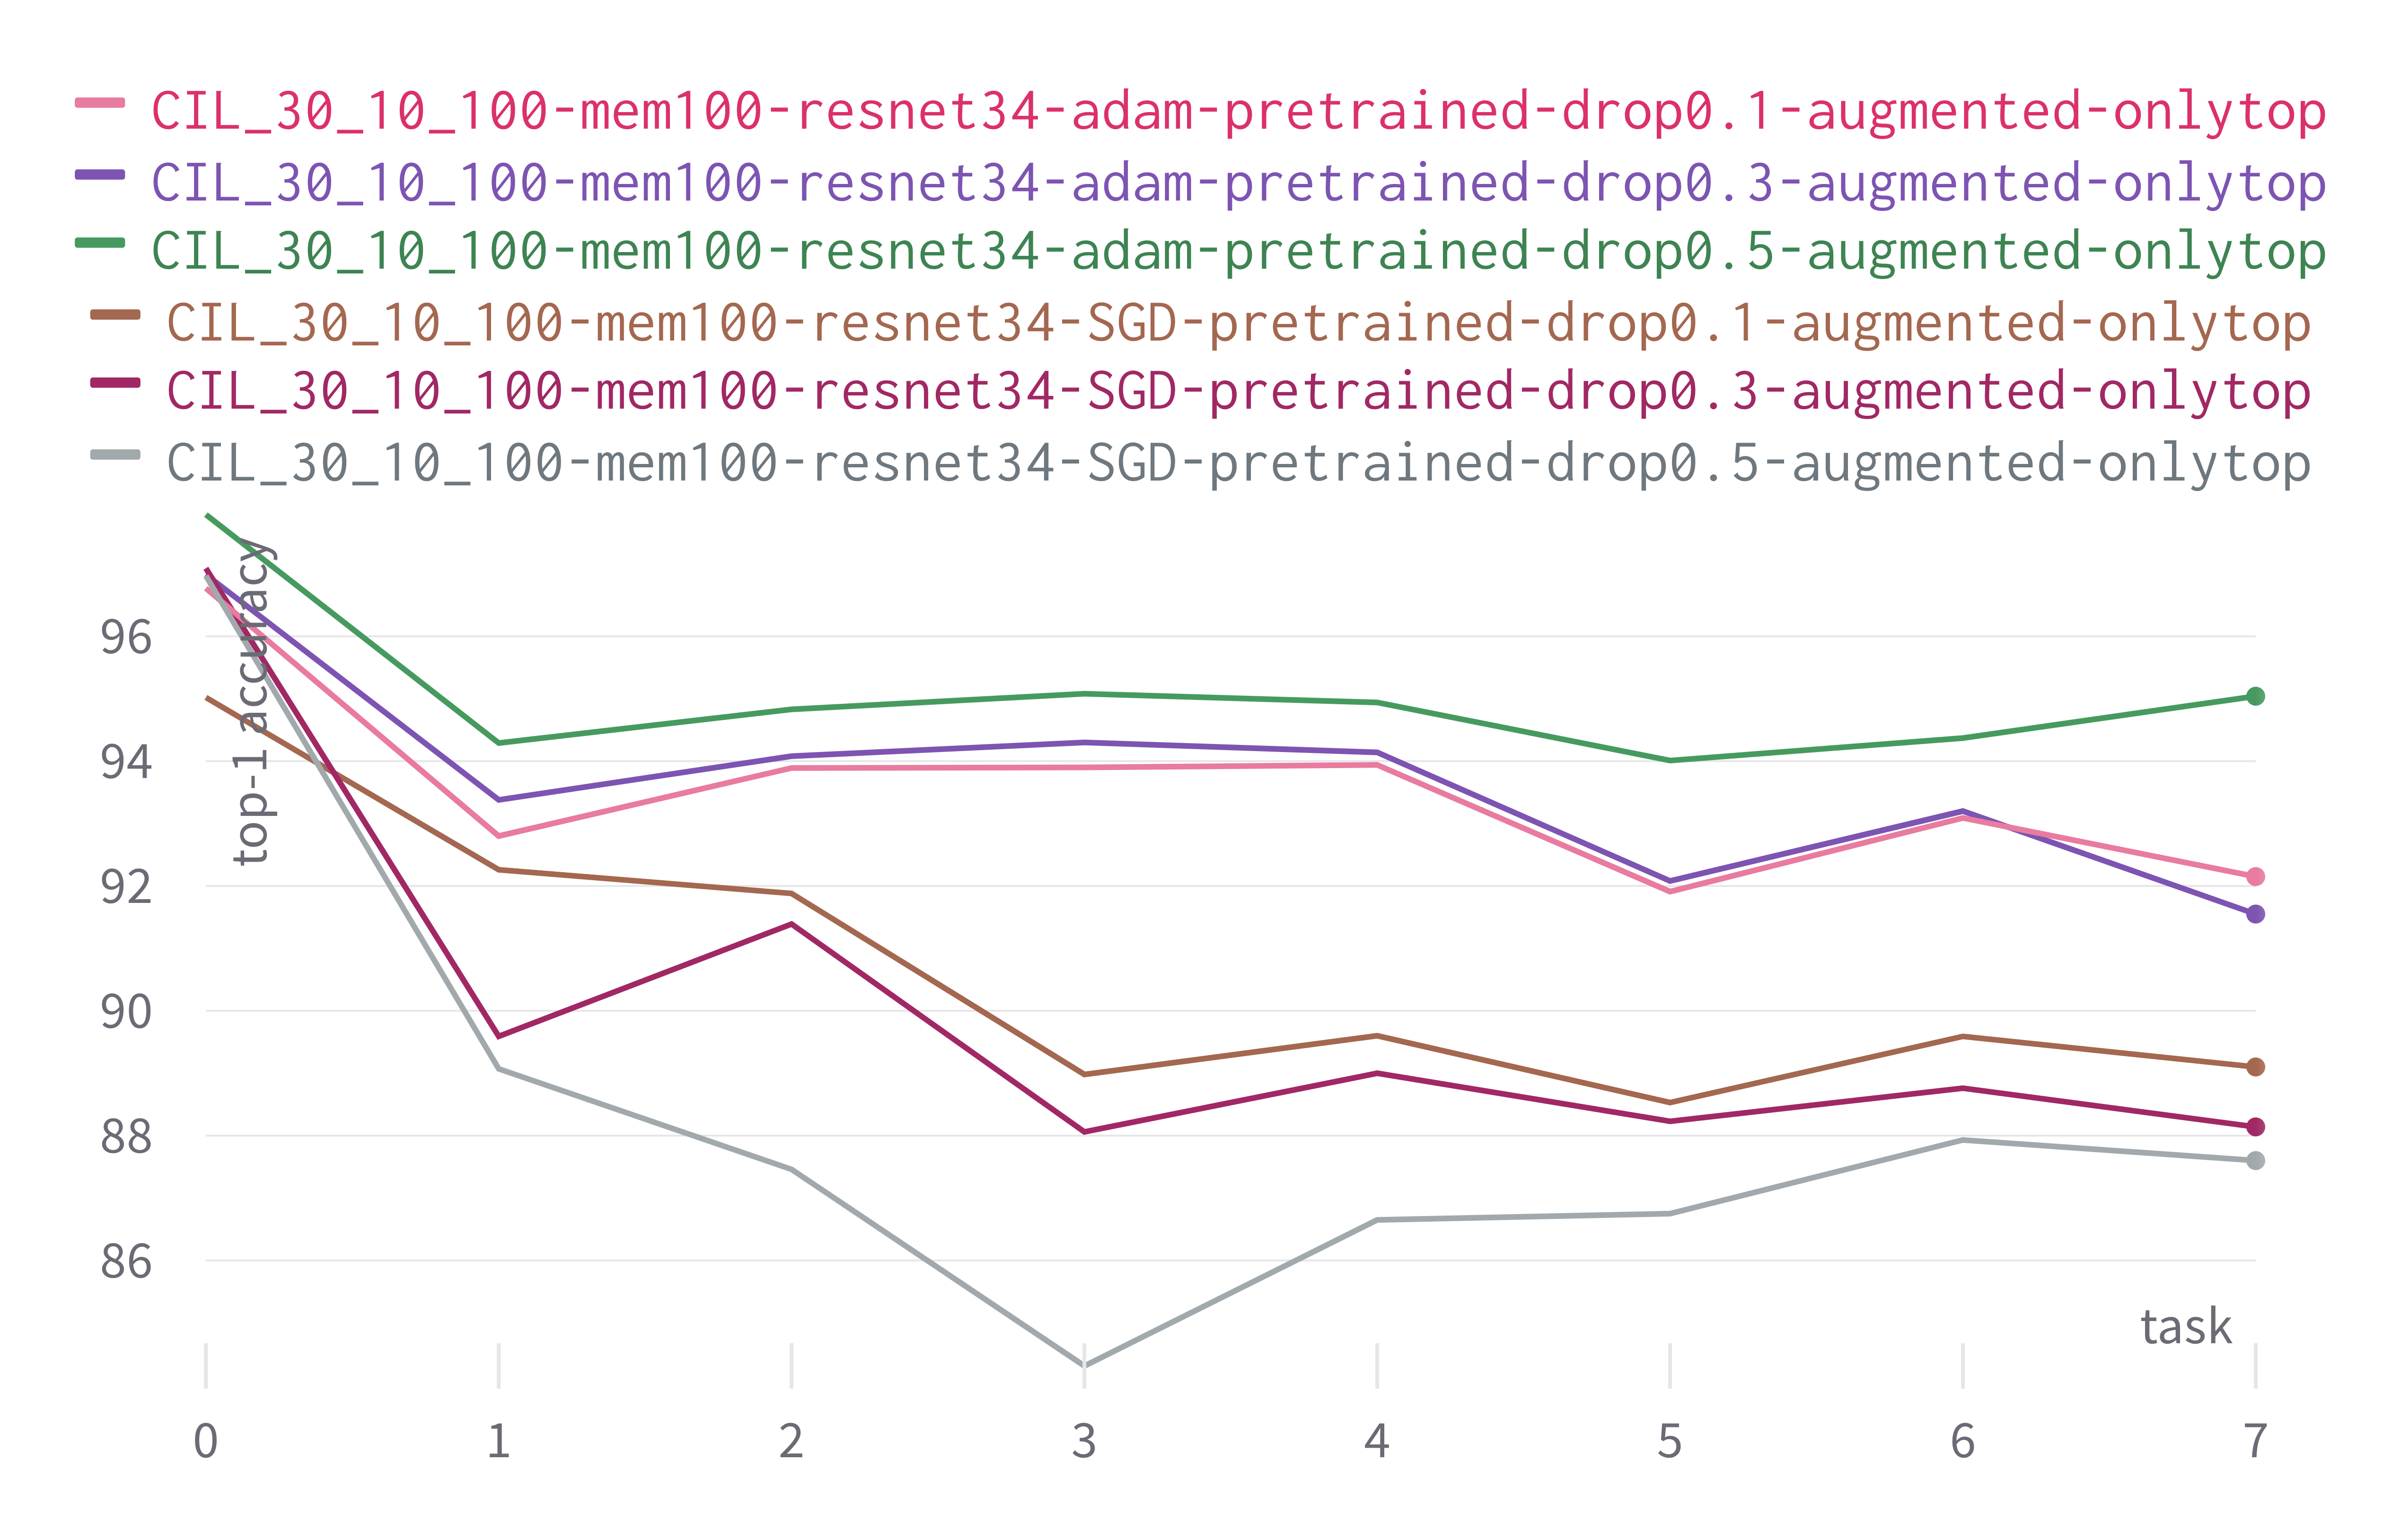
\includegraphics[width=0.80\textwidth]{images/exp/exp4-top1.png} }}%
    \qquad
	\subfloat[\centering Top-5 accuracy]{{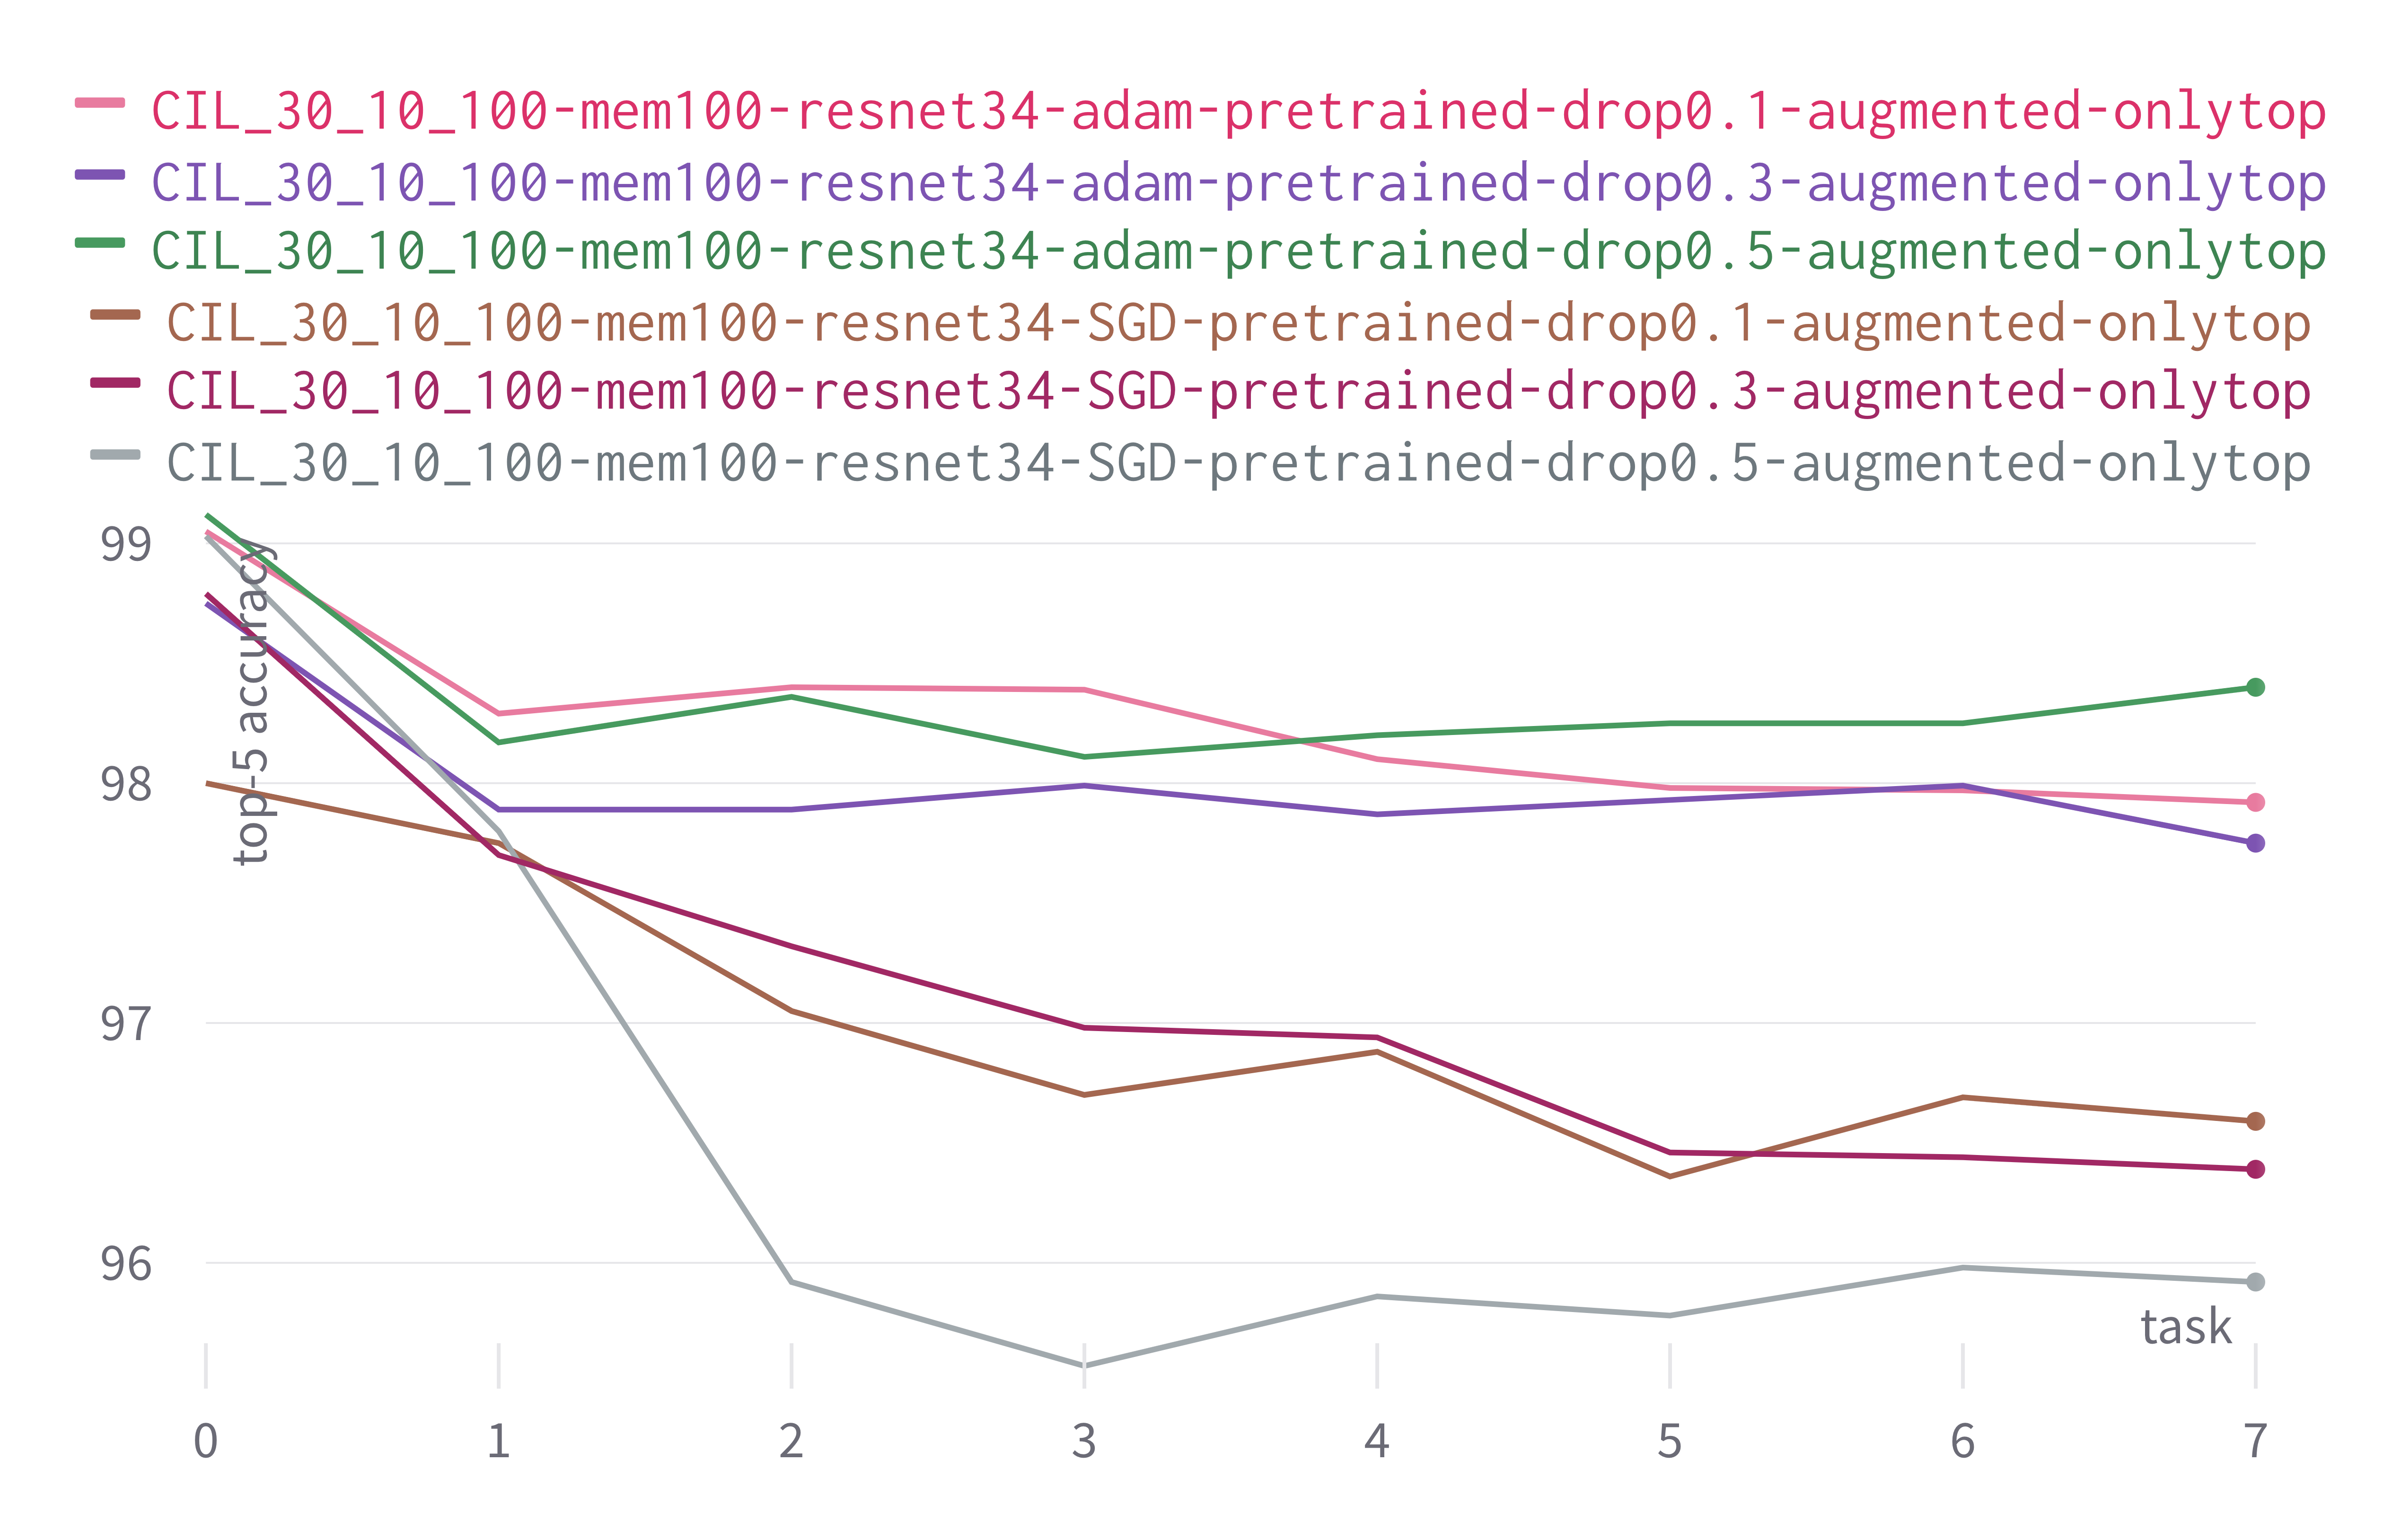
\includegraphics[width=0.80\textwidth]{images/exp/exp4-top5.png} }}%
	\caption{Comparison of models trained using SGD and Adam.}%
	\label{fig:exp4}%
\end{figure}

\begin{figure}[H]
	\centering
	\subfloat[\centering Accuracy on the training set]{{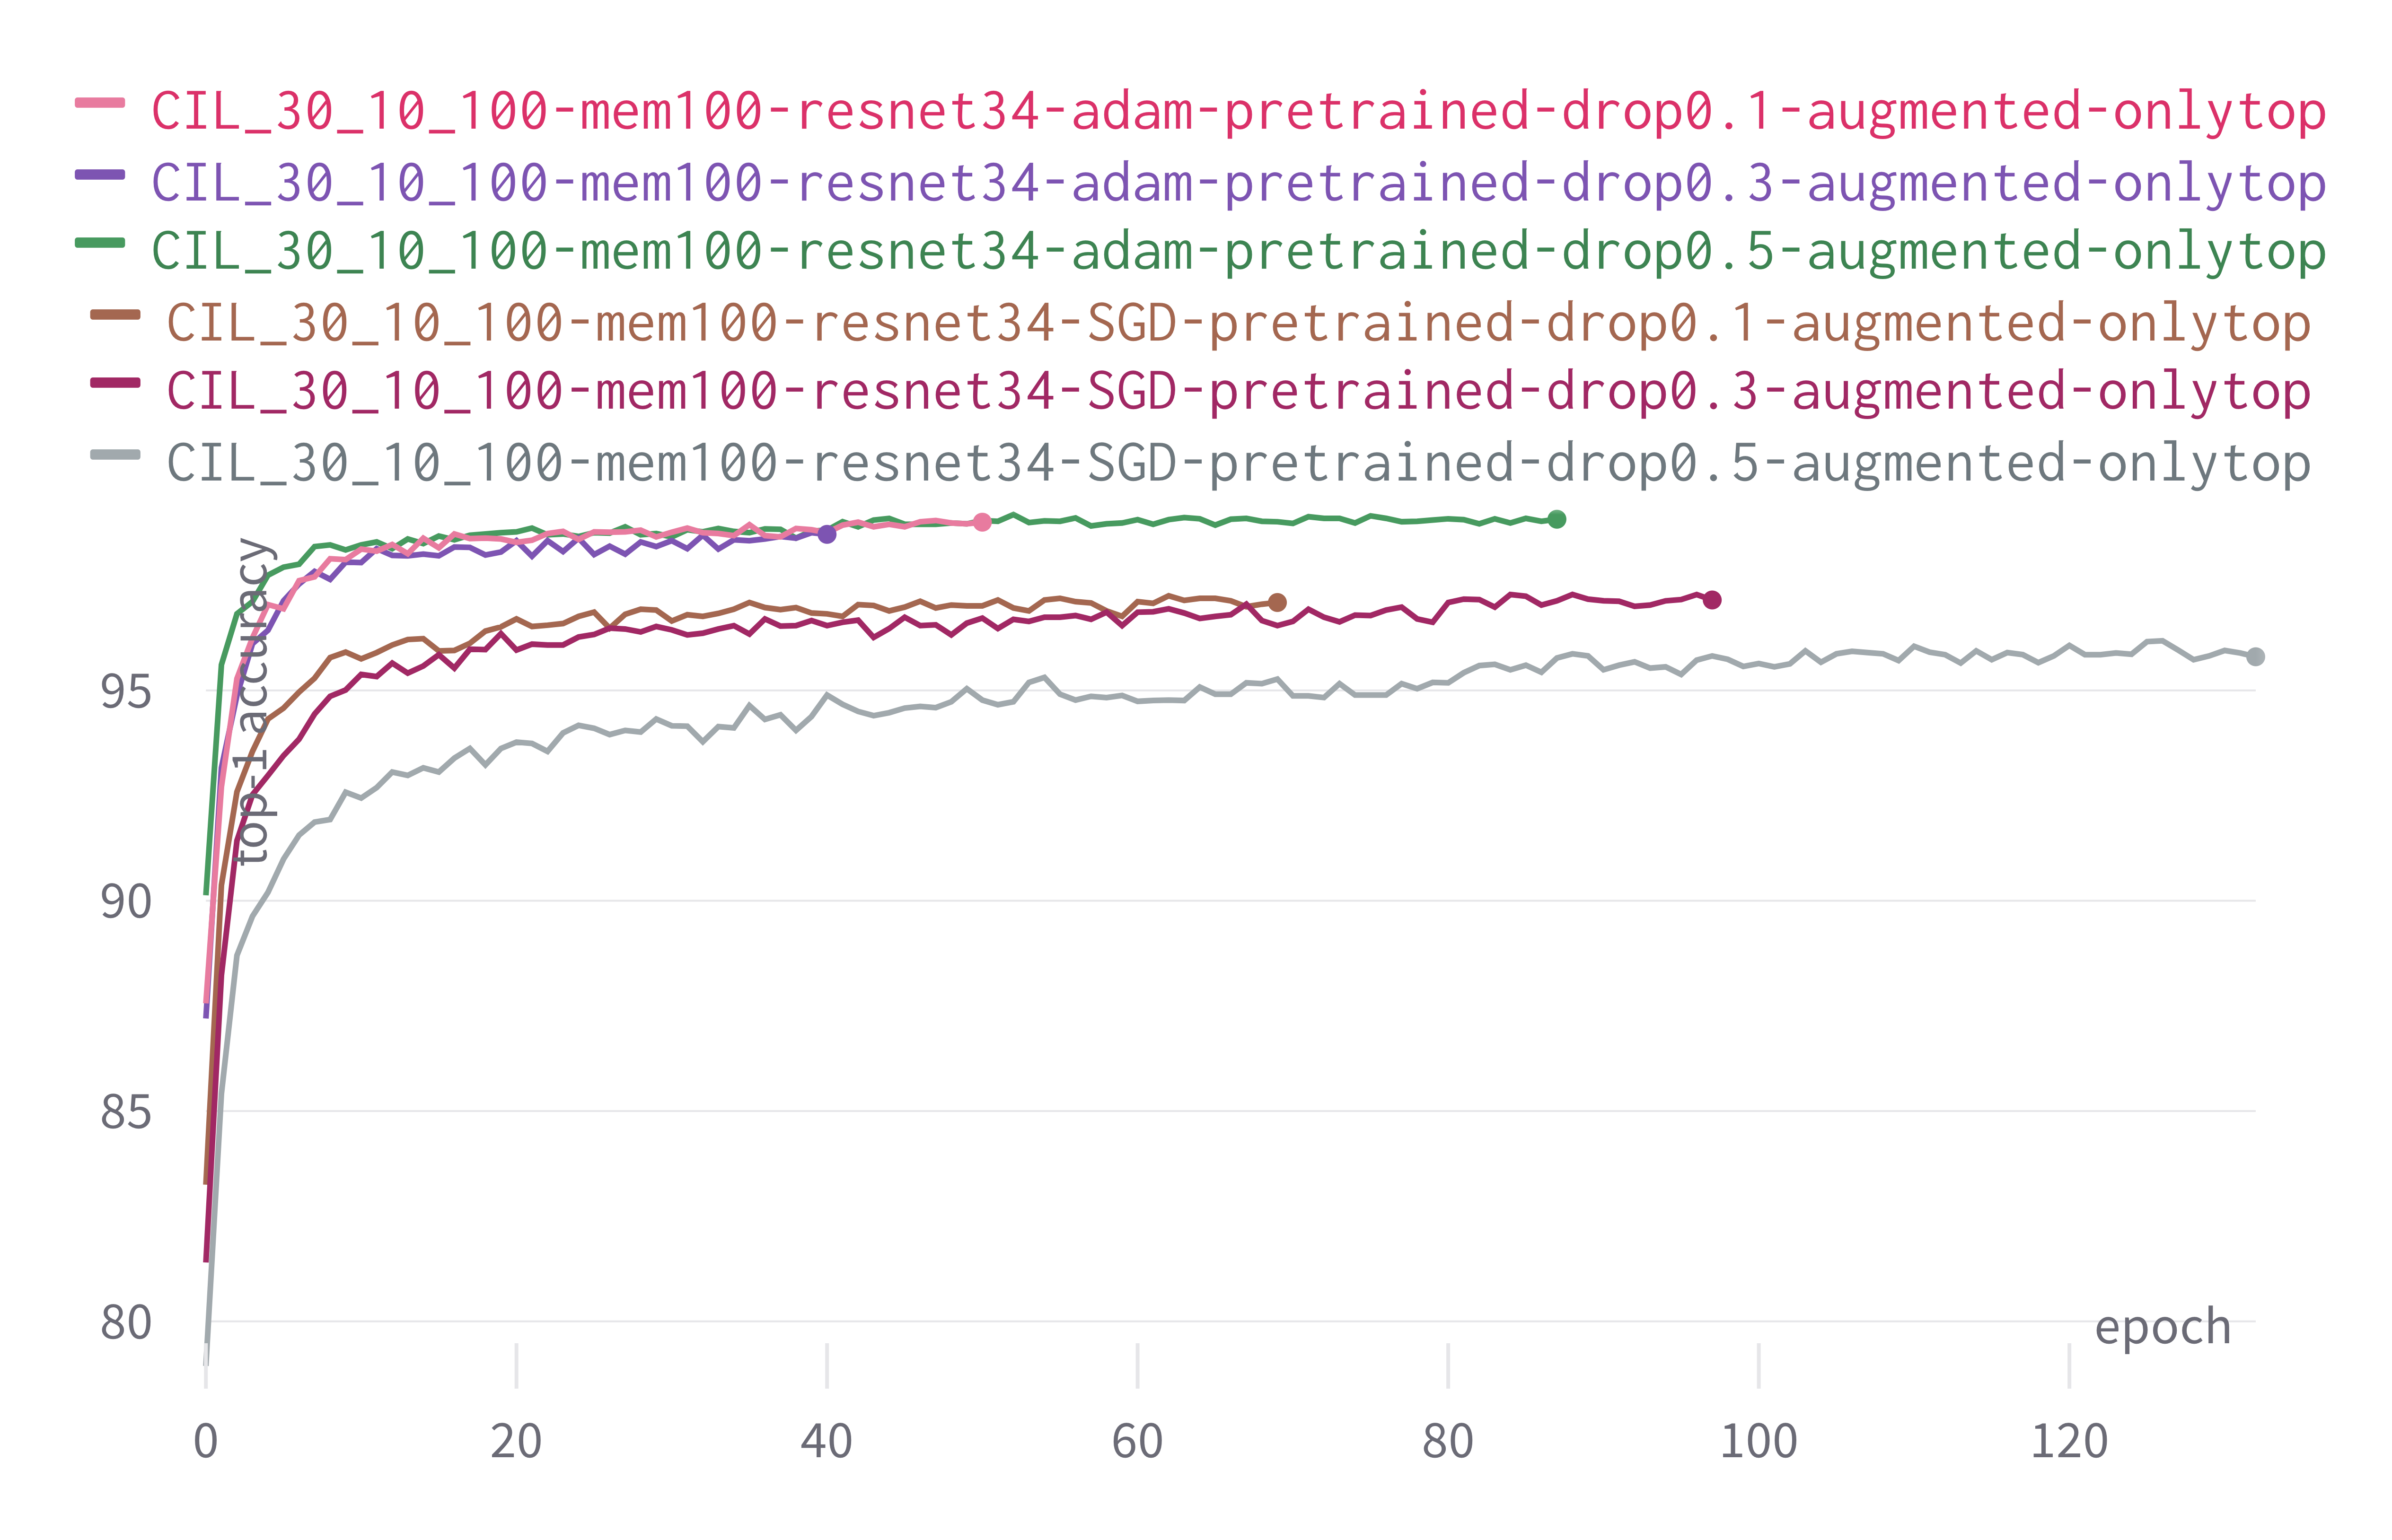
\includegraphics[width=0.80\textwidth]{images/exp/exp4-train.png} }}%
    \qquad
	\subfloat[\centering Accuracy on the validation set]{{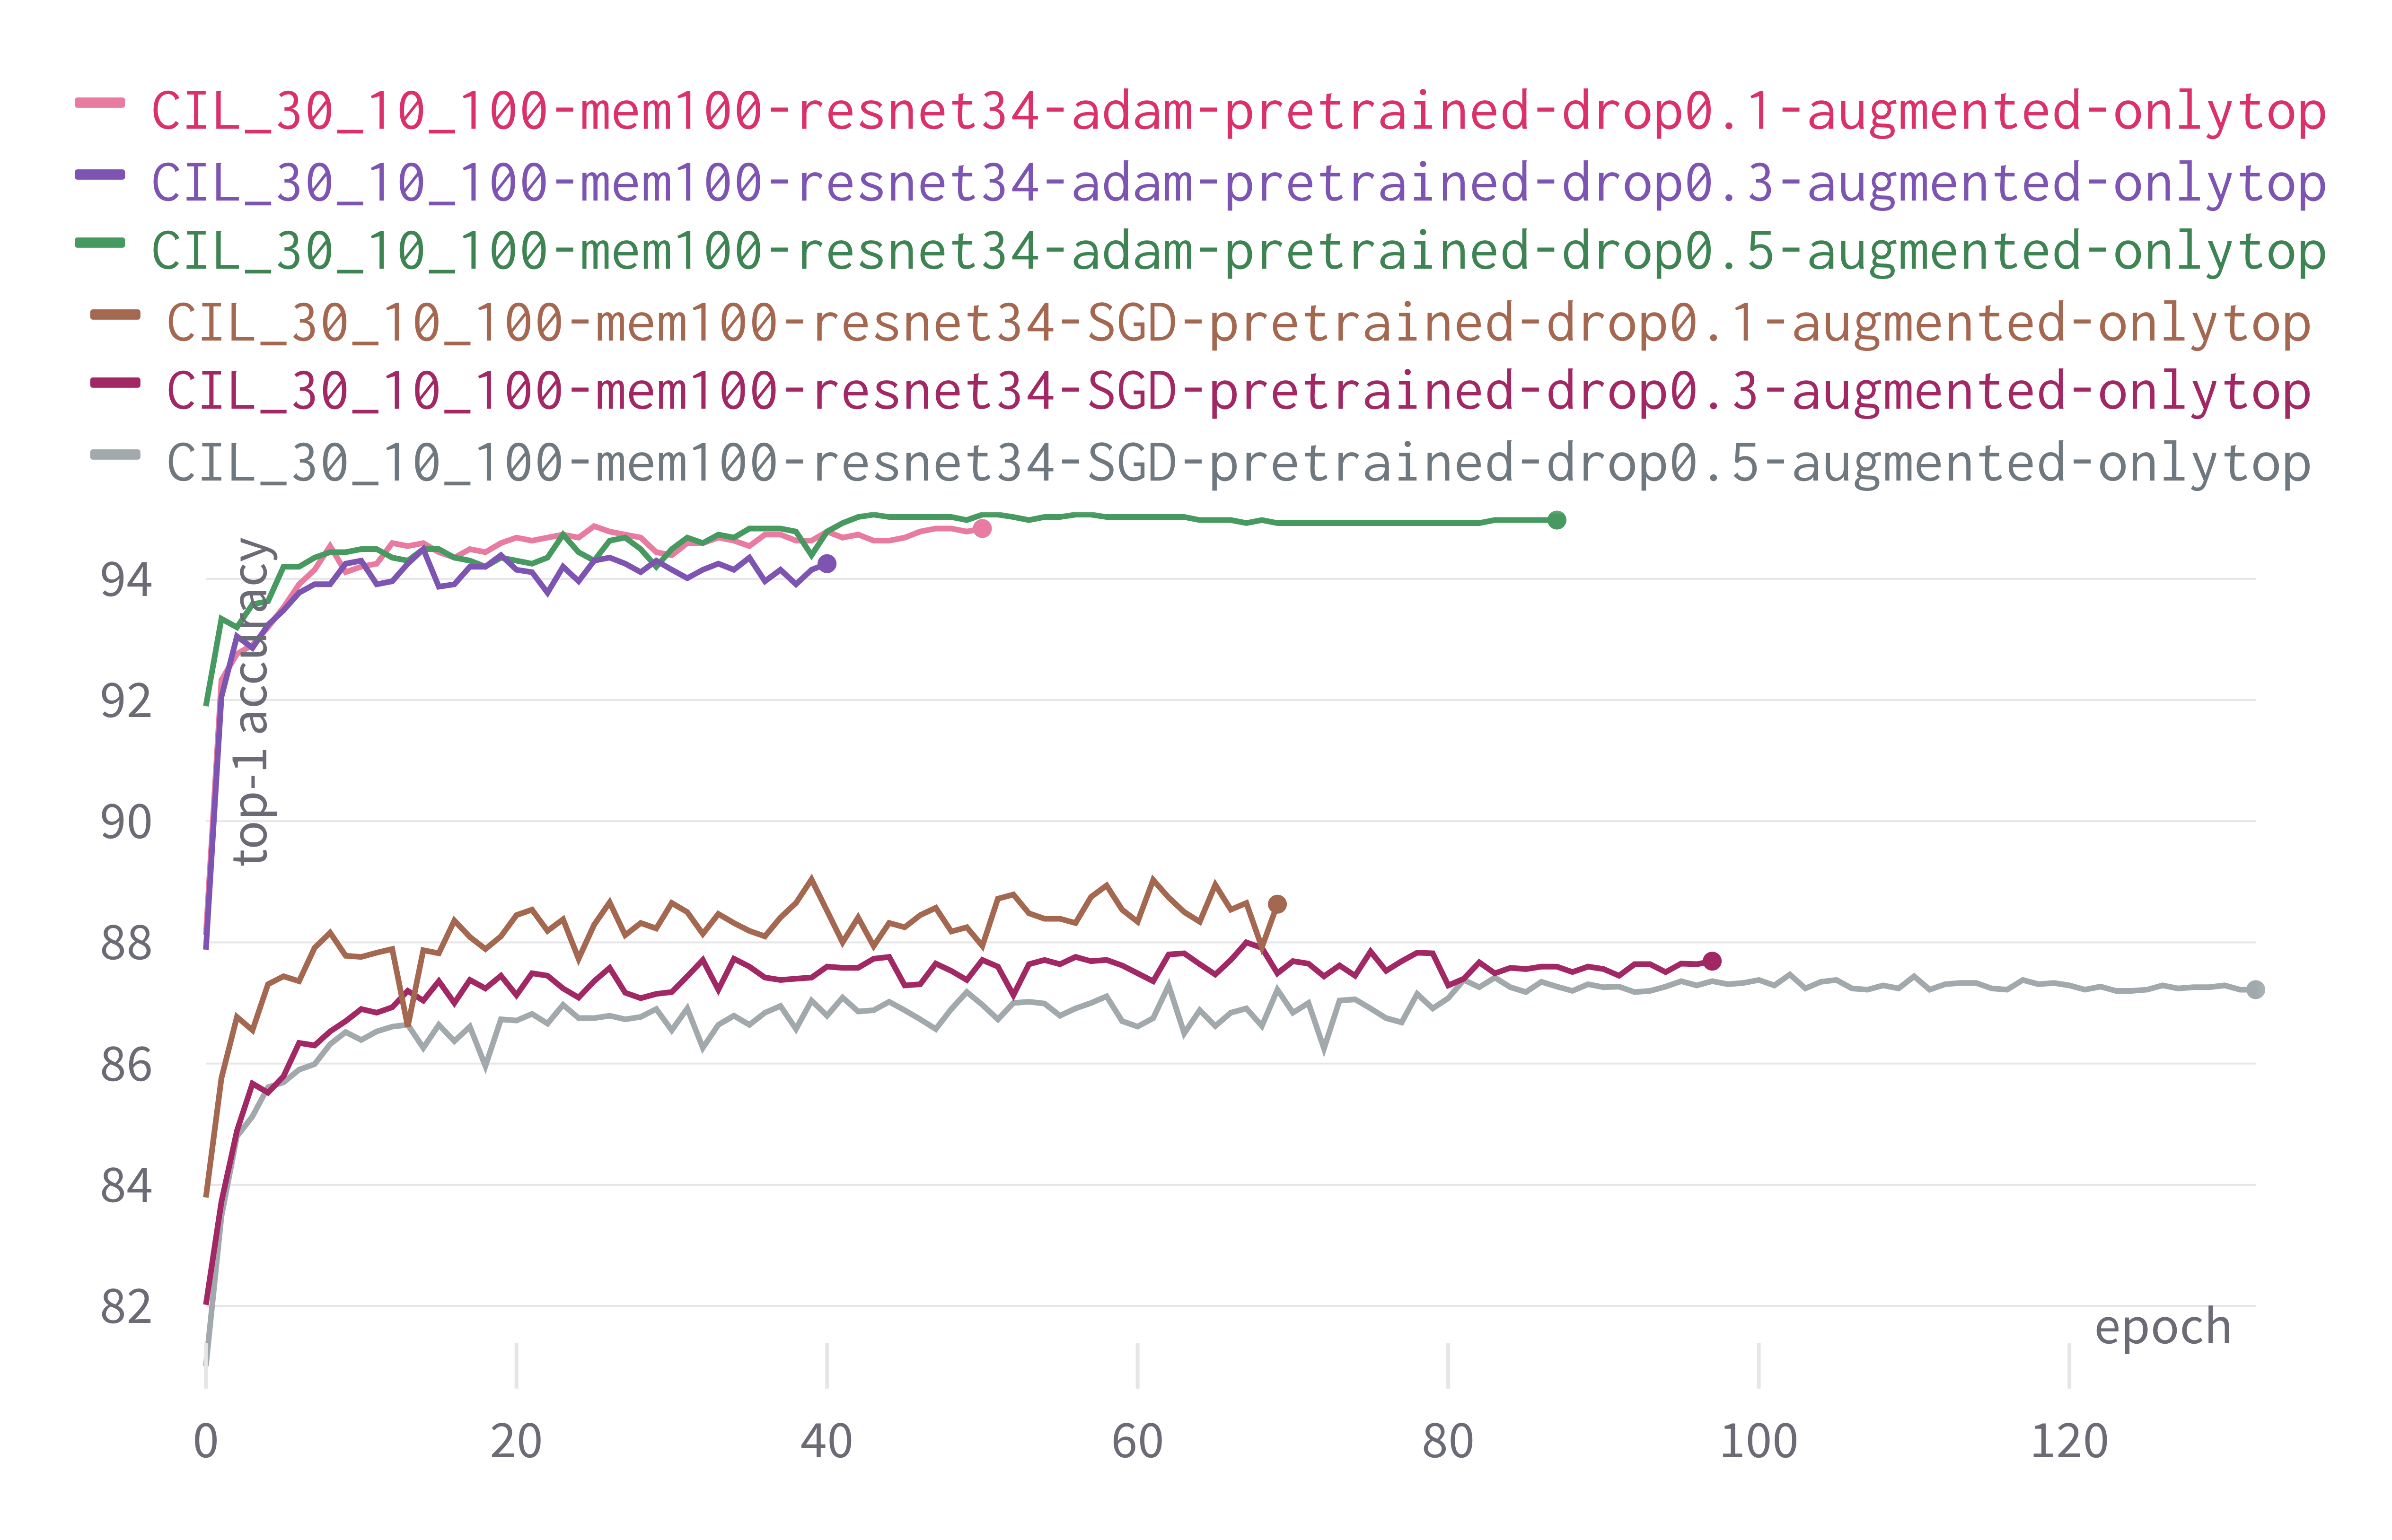
\includegraphics[width=0.80\textwidth]{images/exp/exp4-val.png} }}%
	\caption{Models trained using SGD and Adam: comparison of the accuracy at each training epoch at task 7 between the validation and training set.}%
	\label{fig:exp4-train_val}%
\end{figure}

\newpage


\newpage
\subsubsection{Type 2 baseline}
To address the problems relative to the type 1 baseline, the models tested in the previous section are compared to the 'type 2 baseline' described in \autoref{sec:method-baseline2}. This new baseline is trained on the same dataset used for CIL models and consists in fine-tuning ResNet-152 pretrained on ImageNet to the task of logo classification. This new baseline uses data augmentation, a dropout layer before the FC layer and the Adam optimizer.

Considering the top-1 and top-5 accuracy on the test set, the performance of CIL models and the type 2 baselines is compared in \autoref{table:baseline2}.
As we can see, the performance of the best CIL model is very similar to that of the baseline, but the latter still performs worse, even if slightly.
Although this new baseline mitigates the problem of the number of model parameters, this is still present, as shown in \autoref{table:baseline2-params}.

\begin{table}[H]
    \centering
    \centerline{
    \begin{tabular}{c|c|c}
        \hline
        \textbf{Model} &
        \textbf{Dropout} &
        \textbf{Top-1} \\
        \textbf{name} &
        \textbf{rate} &
        \textbf{acc. (\%)} \\
        \hline
\hline
adam-drop0.1-augmented-onlytop&0.1&92.15\\
adam-drop0.3-augmented-onlytop&0.3&91.55\\
adam-drop0.5-augmented-onlytop&0.5&\textbf{95.04}\\
\hline
BASELINE\_2-drop0.1-augmented-onlytop&0.1&82.35\\
BASELINE\_2-drop0.3-augmented-onlytop&0.3&94.11\\
BASELINE\_2-drop0.5-augmented-onlytop&0.5&88.23\\
\hline 
    \end{tabular}}
    \caption{Performance comparison between the CIL model and the type 2 baseline. Top-1 accuracy tested on 100 classes.}
    \label{table:baseline2}
\end{table}

\begin{table}[H]
    \centering
    \centerline{
    \begin{tabular}{c|c}
        \hline
        \textbf{Model} &
        \textbf{\#Params} \\
        \textbf{name} &
        \textbf{(M)} \\
        \hline
adam-drop0.1-augmented-onlytop&170\\
adam-drop0.3-augmented-onlytop&170\\
adam-drop0.5-augmented-onlytop&170\\
\hline
BASELINE\_2-drop0.1-augmented-onlytop&60\\
BASELINE\_2-drop0.3-augmented-onlytop&60\\
BASELINE\_2-drop0.5-augmented-onlytop&60\\
\hline 
    \end{tabular}}
    \caption{Number of model parameters between the CIL model and the typ 2 baseline.}
    \label{table:baseline2-params}
\end{table}

\newpage
\subsubsection{Type 3 baseline}
This third baseline, 'type 3 baseline' aims to solve the problem of the number of model parameters. In fact, this approach, described in \autoref{sec:method-baseline3}, defines the baseline architecture using the DER algorithm in the exact same setup as the CIL classifier, thus having an identical architecture of the CIL model and the baseline.
This ensures that the number of model parameters is the same.
Therefore, the baseline is trained using the same dataset, data augmentation, regularization, and the Adam optimizer.

The performance between the CIL models and this new baseline is compared considering the top-1 on the test set. As we can see from \autoref{table:baseline3}, the type 3 baseline achieves better performance than the CIL model.

This makes it possible to compare the actual drop in performance using an incremental learning setup compared to a standard setup.
As shown in \autoref{table:baseline3}, this gap is present, with a 3\% drop in top-1 accuracy, but it is expected using an incremental learning setup.
However, a 3\% drop is acceptable when considering the advantages of an incremental learning approach.

\begin{table}[H]
    \centering
    \centerline{
    \begin{tabular}{c|c|c|c}
        \hline
        \textbf{Model} &
        \textbf{Dropout} &
        \textbf{Top-1} \\
        \textbf{name} &
        \textbf{rate} &
        \textbf{acc. (\%)} \\
        \hline
\hline
adam-drop0.1-augmented-onlytop&0.1&92.15\\
adam-drop0.3-augmented-onlytop&0.3&91.55\\
adam-drop0.5-augmented-onlytop&0.5&95.04\\
\hline\
BASELINE\_3-drop0.1-augmented-onlytop&0.1&\textbf{98.52}\\
BASELINE\_3-drop0.3-augmented-onlytop&0.3&97.05\\
BASELINE\_3-drop0.5-augmented-onlytop&0.5&97.64\\
\hline 
    \end{tabular}}
    \caption{Top-1 accuracy of the CIL model and the type 3 baseline consider all the 100 classes of the test set.}
    \label{table:baseline3}
\end{table}

\newpage
\subsubsection{Pruning (100 classes)}
An important aspect discussed in \autoref{sec:method-pruning} is the number of model parameters. All the models tested up to this point add approximately 22 million parameters with each new incremental iteration of learning, thus reaching 170 million parameters at task 7 (22 million for the initial task and 7 iterations of incremental learning).

The following experiments are designed to assess the pruning capacity of the channel-level masks and the drop in performance obtained by using this method. To this end, the pruned models are compared to those described in the previous section. An important difference in the training procedure of the pruned model is to monitor the loss on the validation set instead of the validation accuracy. Since the validation loss decreases with increasing sparsity of the model, we want to encourage a sparser model given the same accuracy on the validation set.

The results regarding the performance comparison are shown in \autoref{fig:exp5} and \autoref{table:exp5}. As we can see, the drop in performance is negligible, with some pruned models performing even better than un-pruned ones. This can be explained by considering pruning as a regularization technique, in fact, the number of parameters reduced (effectively reducing the Vapnik-Chervonenkis dimension \cite{vapnik1999nature}). However, it is important to emphasize that these models are trained considering the top-100 classes, so it is essential to test the scalability of the models, and also of pruning, to the entire dataset.


\begin{figure}[H]
	\centering
	\subfloat[\centering Top-1 accuracy]{{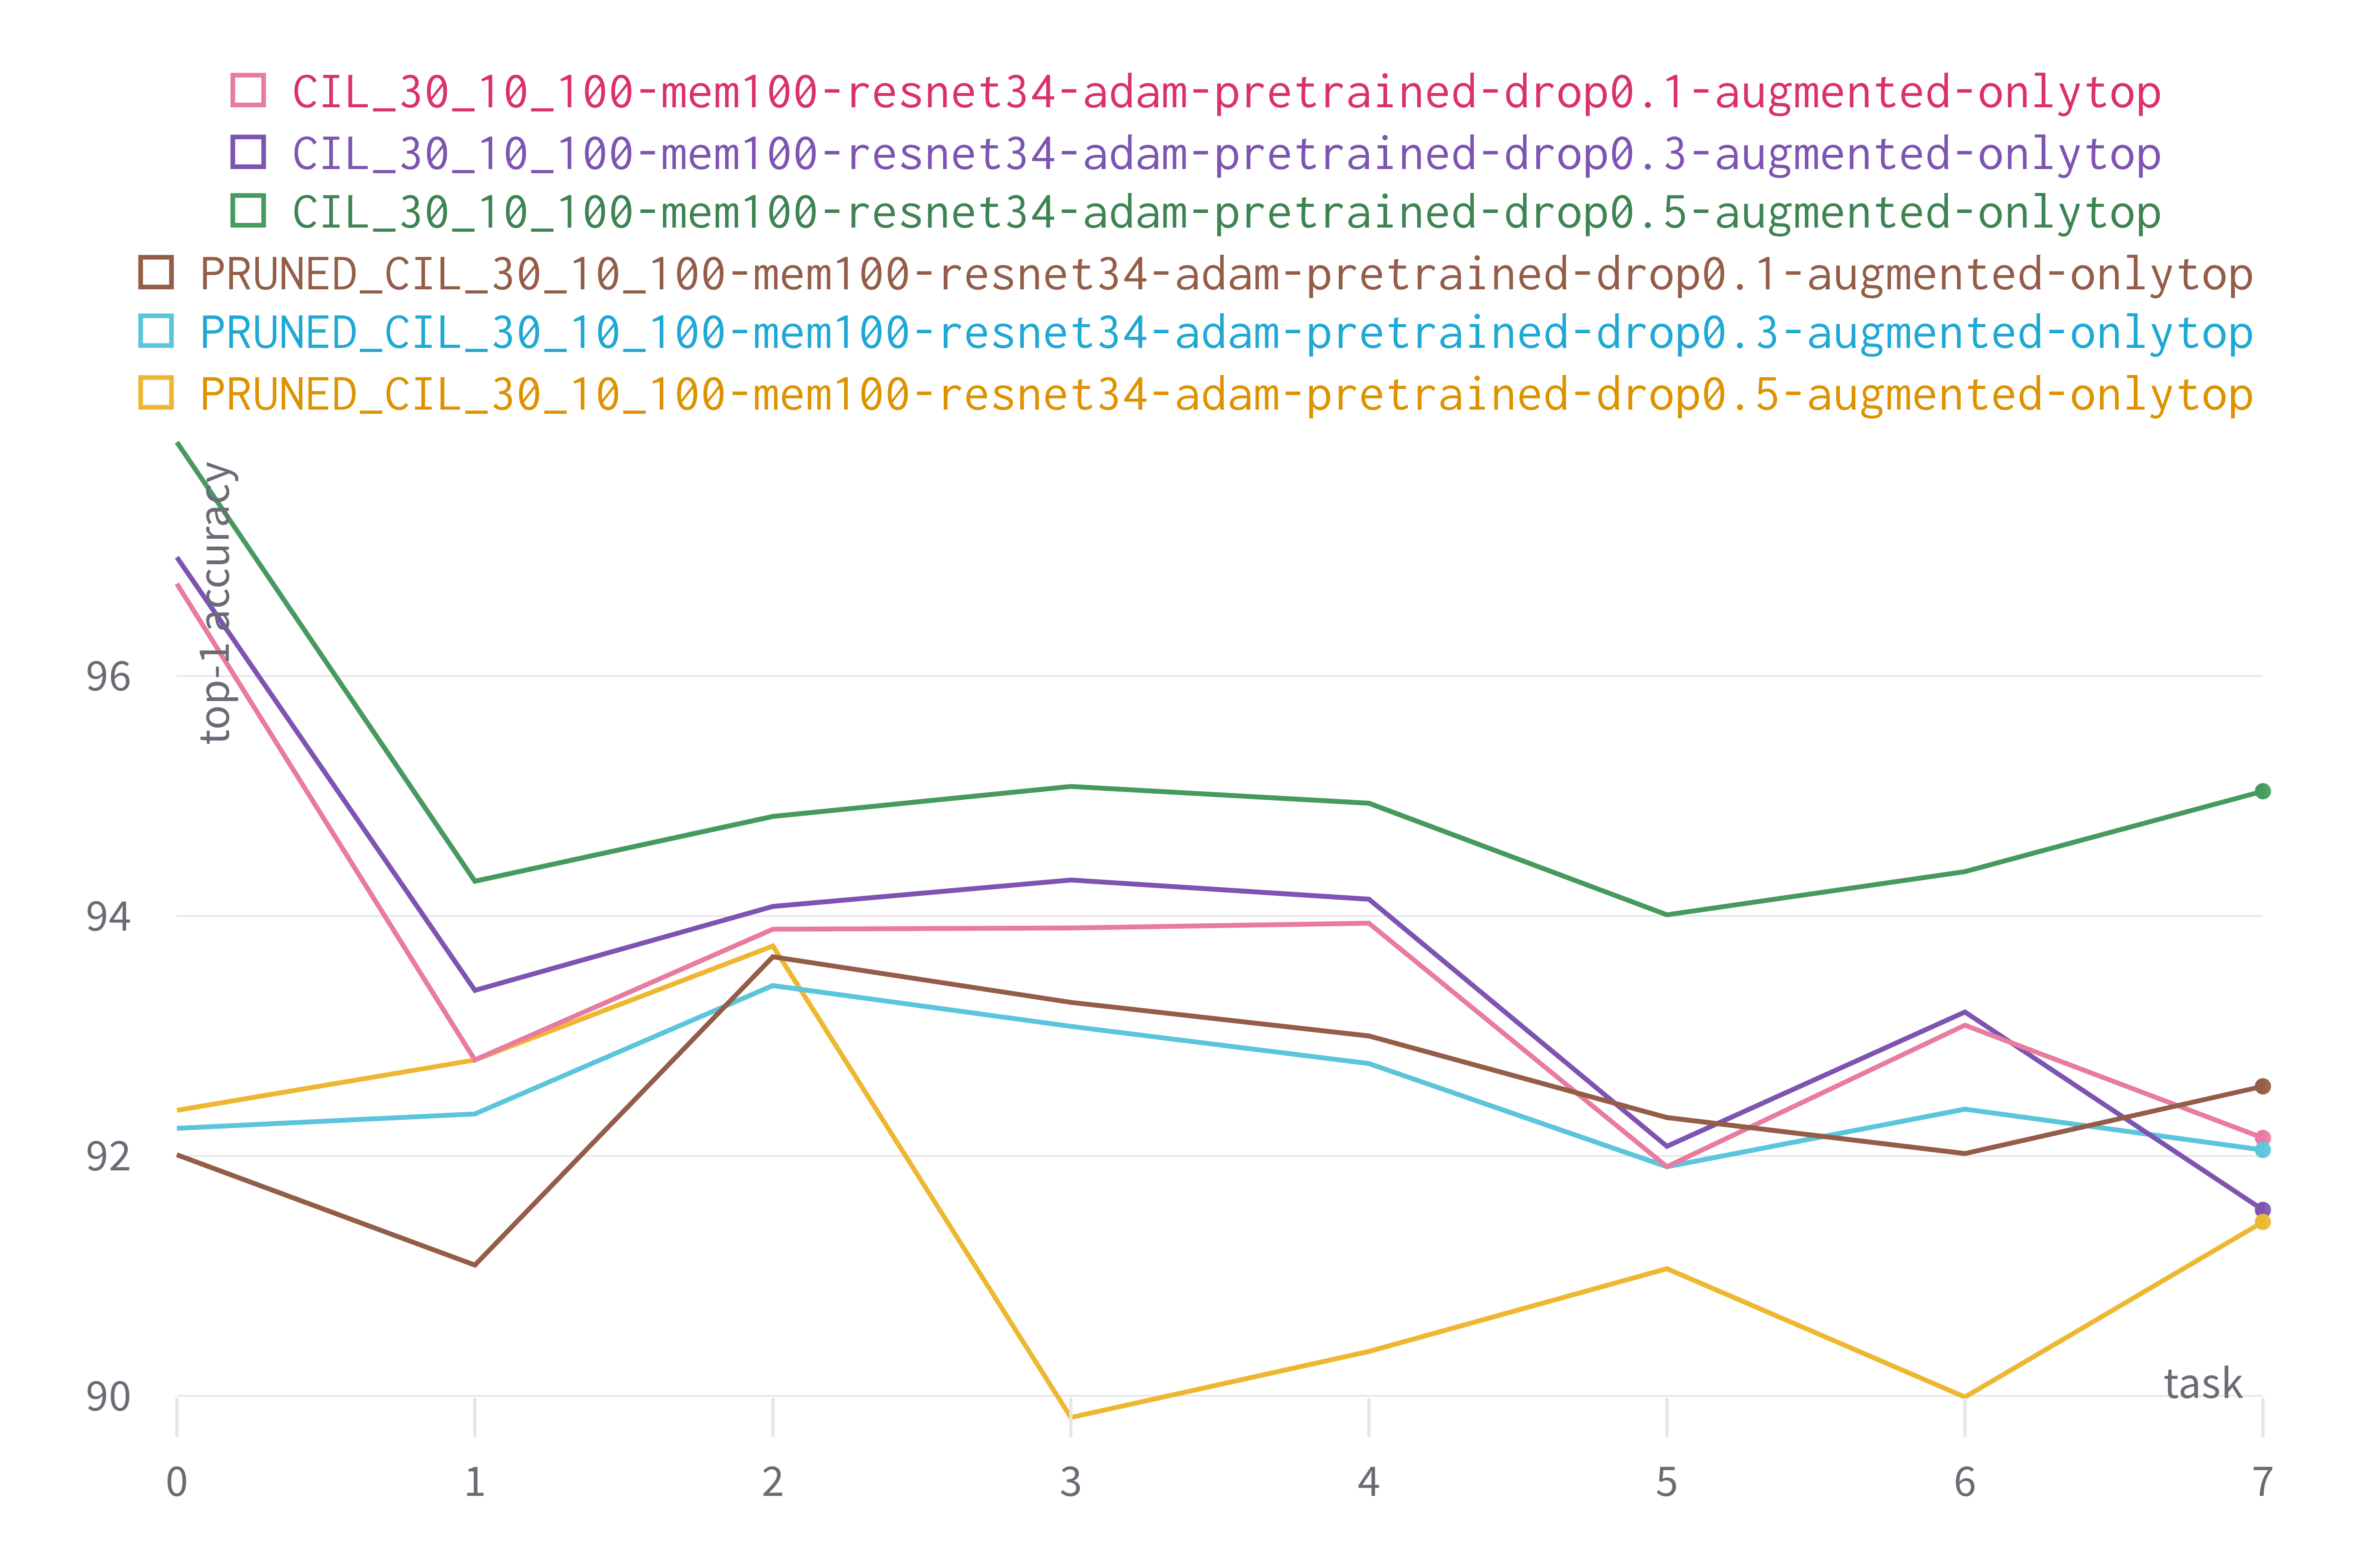
\includegraphics[width=0.80\textwidth]{images/exp/exp5-top1.png} }}%
    \qquad
	\subfloat[\centering Top-5 accuracy]{{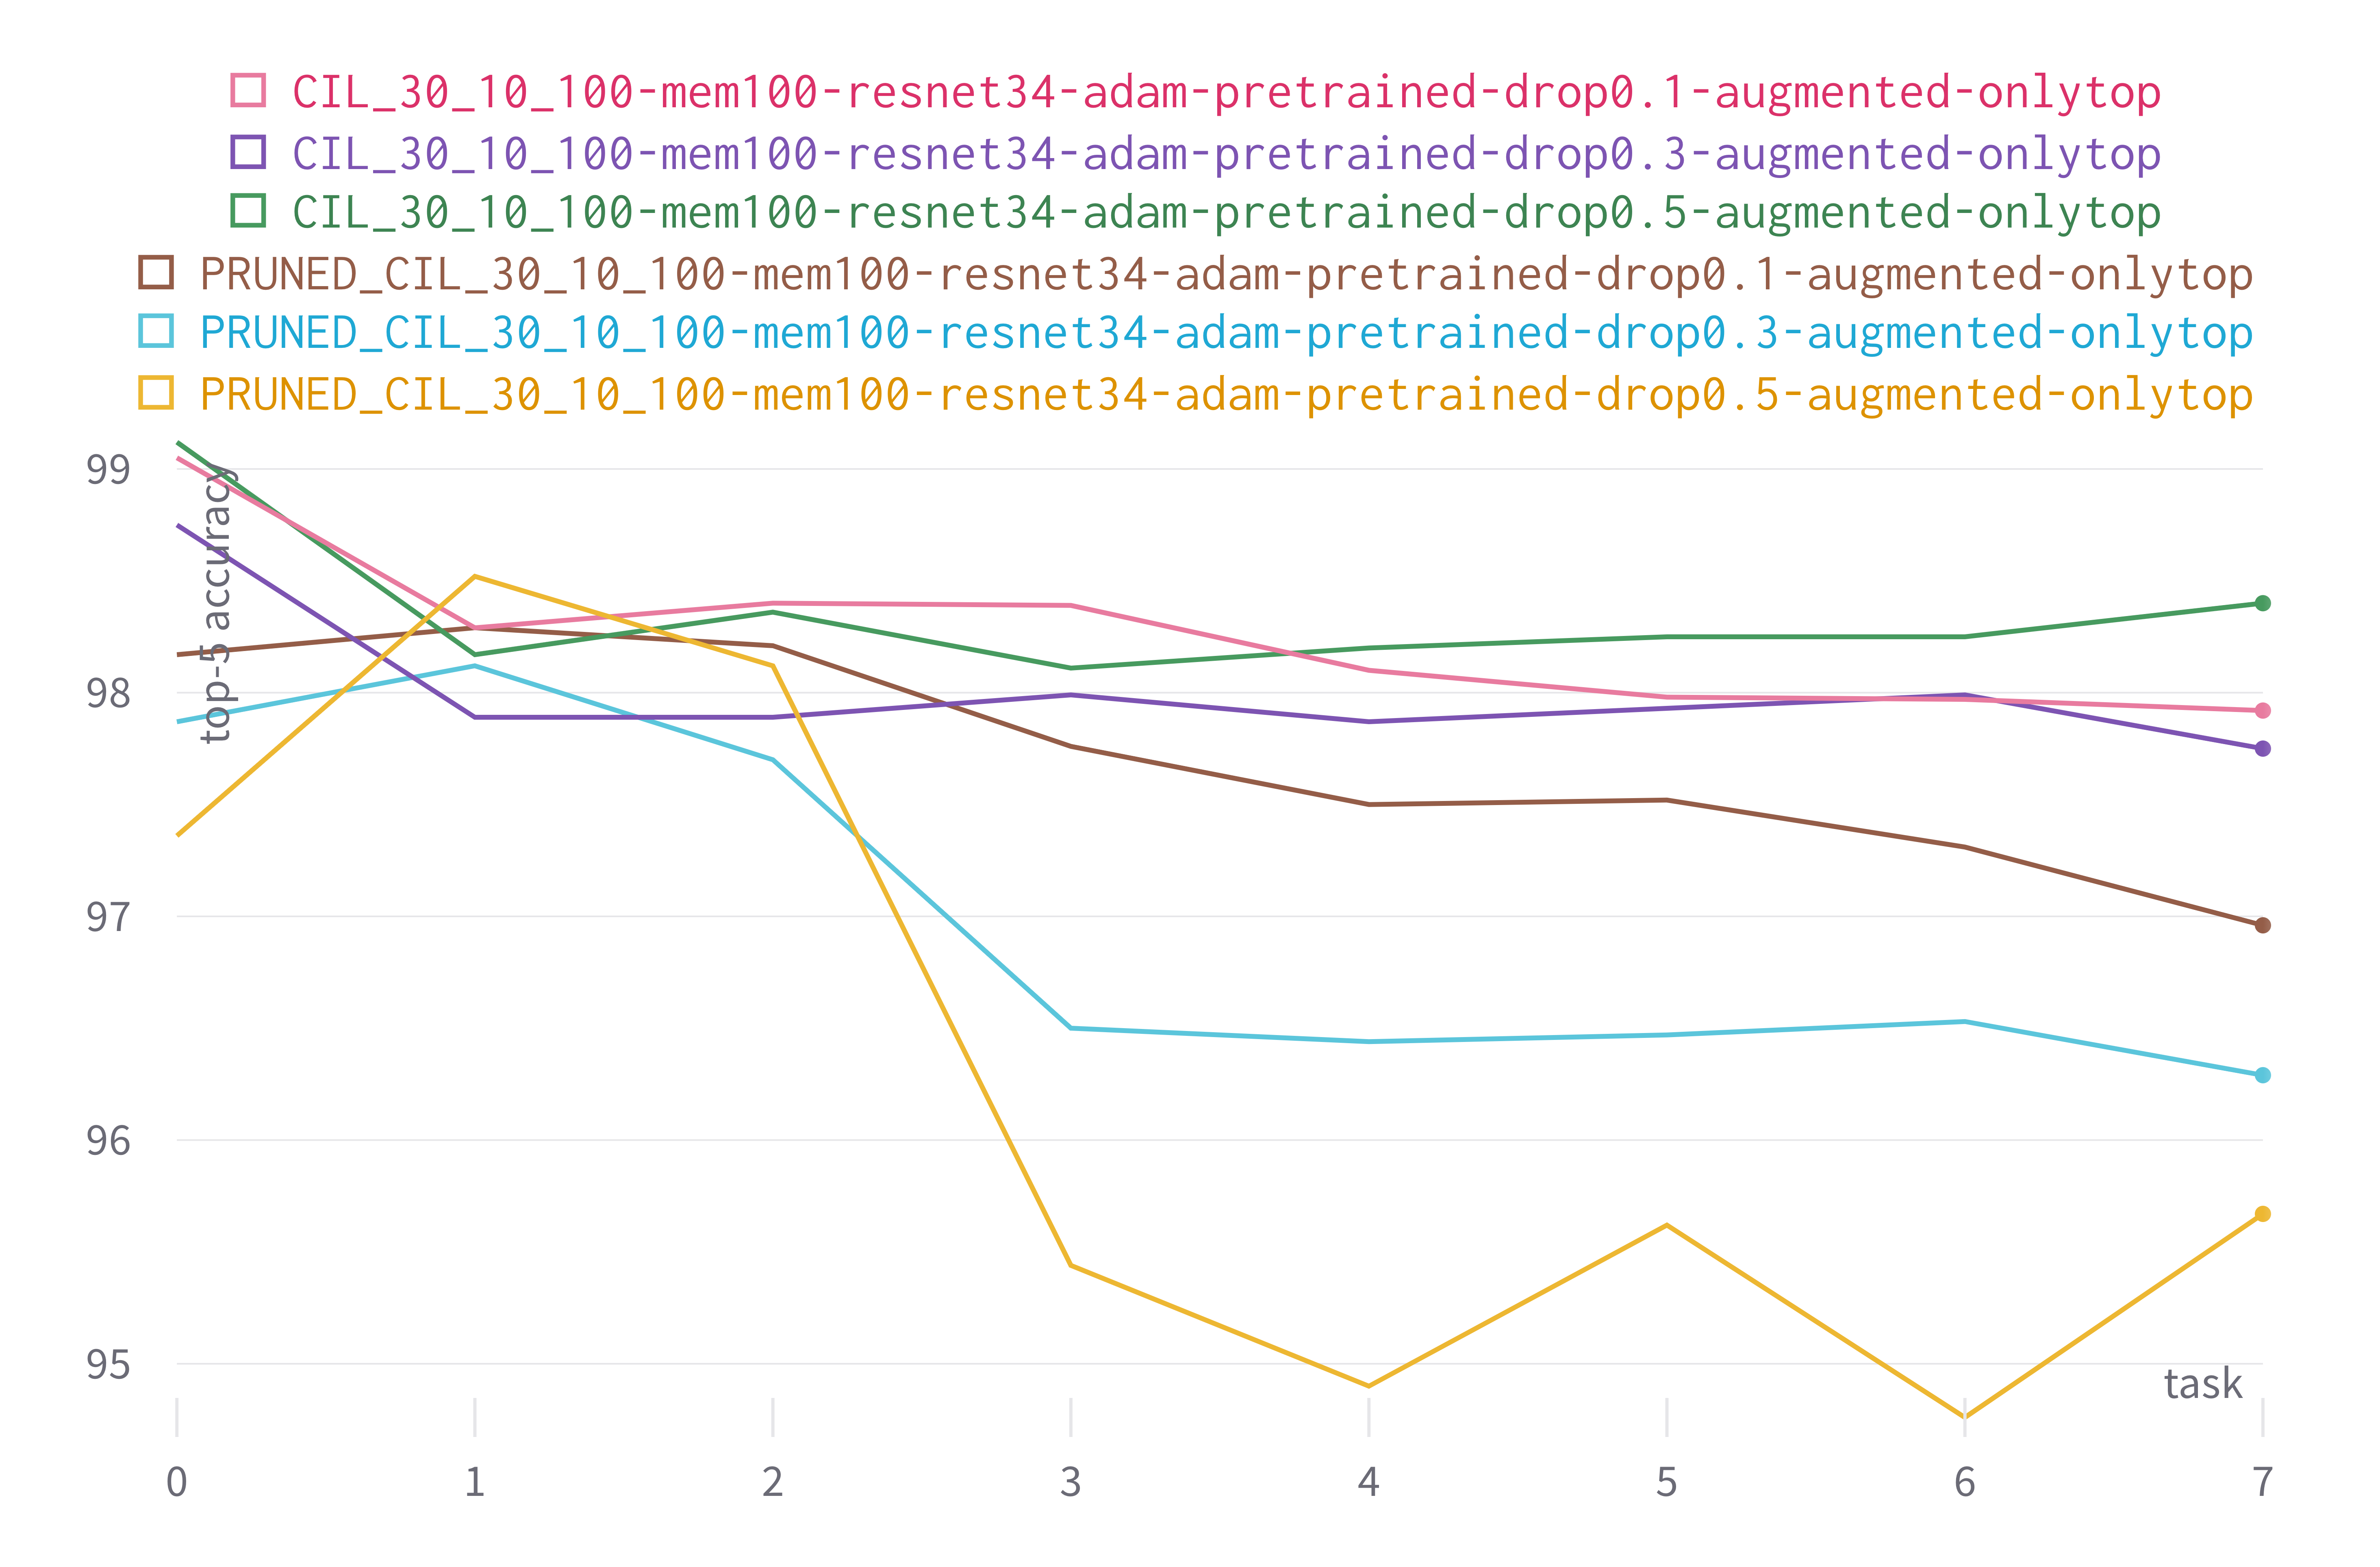
\includegraphics[width=0.80\textwidth]{images/exp/exp5-top5.png} }}%
	\caption{Performance comparison between the pruned model and standard model.}%
	\label{fig:exp5}%
\end{figure}

\begin{table}[H]
    \centering
    \centerline{
    \begin{tabular}{c|c|c|c|c}
        \hline
        \textbf{Model} &
        \textbf{Dropout} &
        \textbf{Pruning} &
        \textbf{Top-1} & 
        \textbf{Top-5} \\
        \textbf{name} &
        \textbf{rate} &
        &
        \textbf{acc. (\%)} & 
        \textbf{acc. (\%)} \\
        \hline
        \hline
drop0.1-augmented-onlytop&0.1&no&92.15&97.92\\
drop0.3-augmented-onlytop&0.3&no&91.55&97.75\\
drop0.5-augmented-onlytop&0.5&no&\textbf{95.04}&\textbf{98.4}\\
\hline
PRUNED-drop0.1-augmented-onlytop&0.1&yes&92.58&96.96\\
PRUNED-drop0.3-augmented-onlytop&0.3&yes&92.05&96.29\\
PRUNED-drop0.5-augmented-onlytop&0.5&yes&91.45&95.67\\
        \hline
    \end{tabular}}
    \caption{Performance comparison between the pruned models and the un-pruned ones. Top-1 accuracy at task 7.}
    \label{table:exp5}
\end{table}

The result of pruning regarding the number of parameters is shown in \autoref{fig:exp5-params} and \autoref{table:exp5-params}. As we can see, this technique is very effective. The final number of model parameters is reduced by almost a factor of 5x, the models not using pruning already exceed the total number of parameters of those using pruning for task 1 (43 for the un-pruned vs. 32 for pruned approx.).

\begin{table}[ht]
    \begin{minipage}[b]{0.49\linewidth}
        \centering
        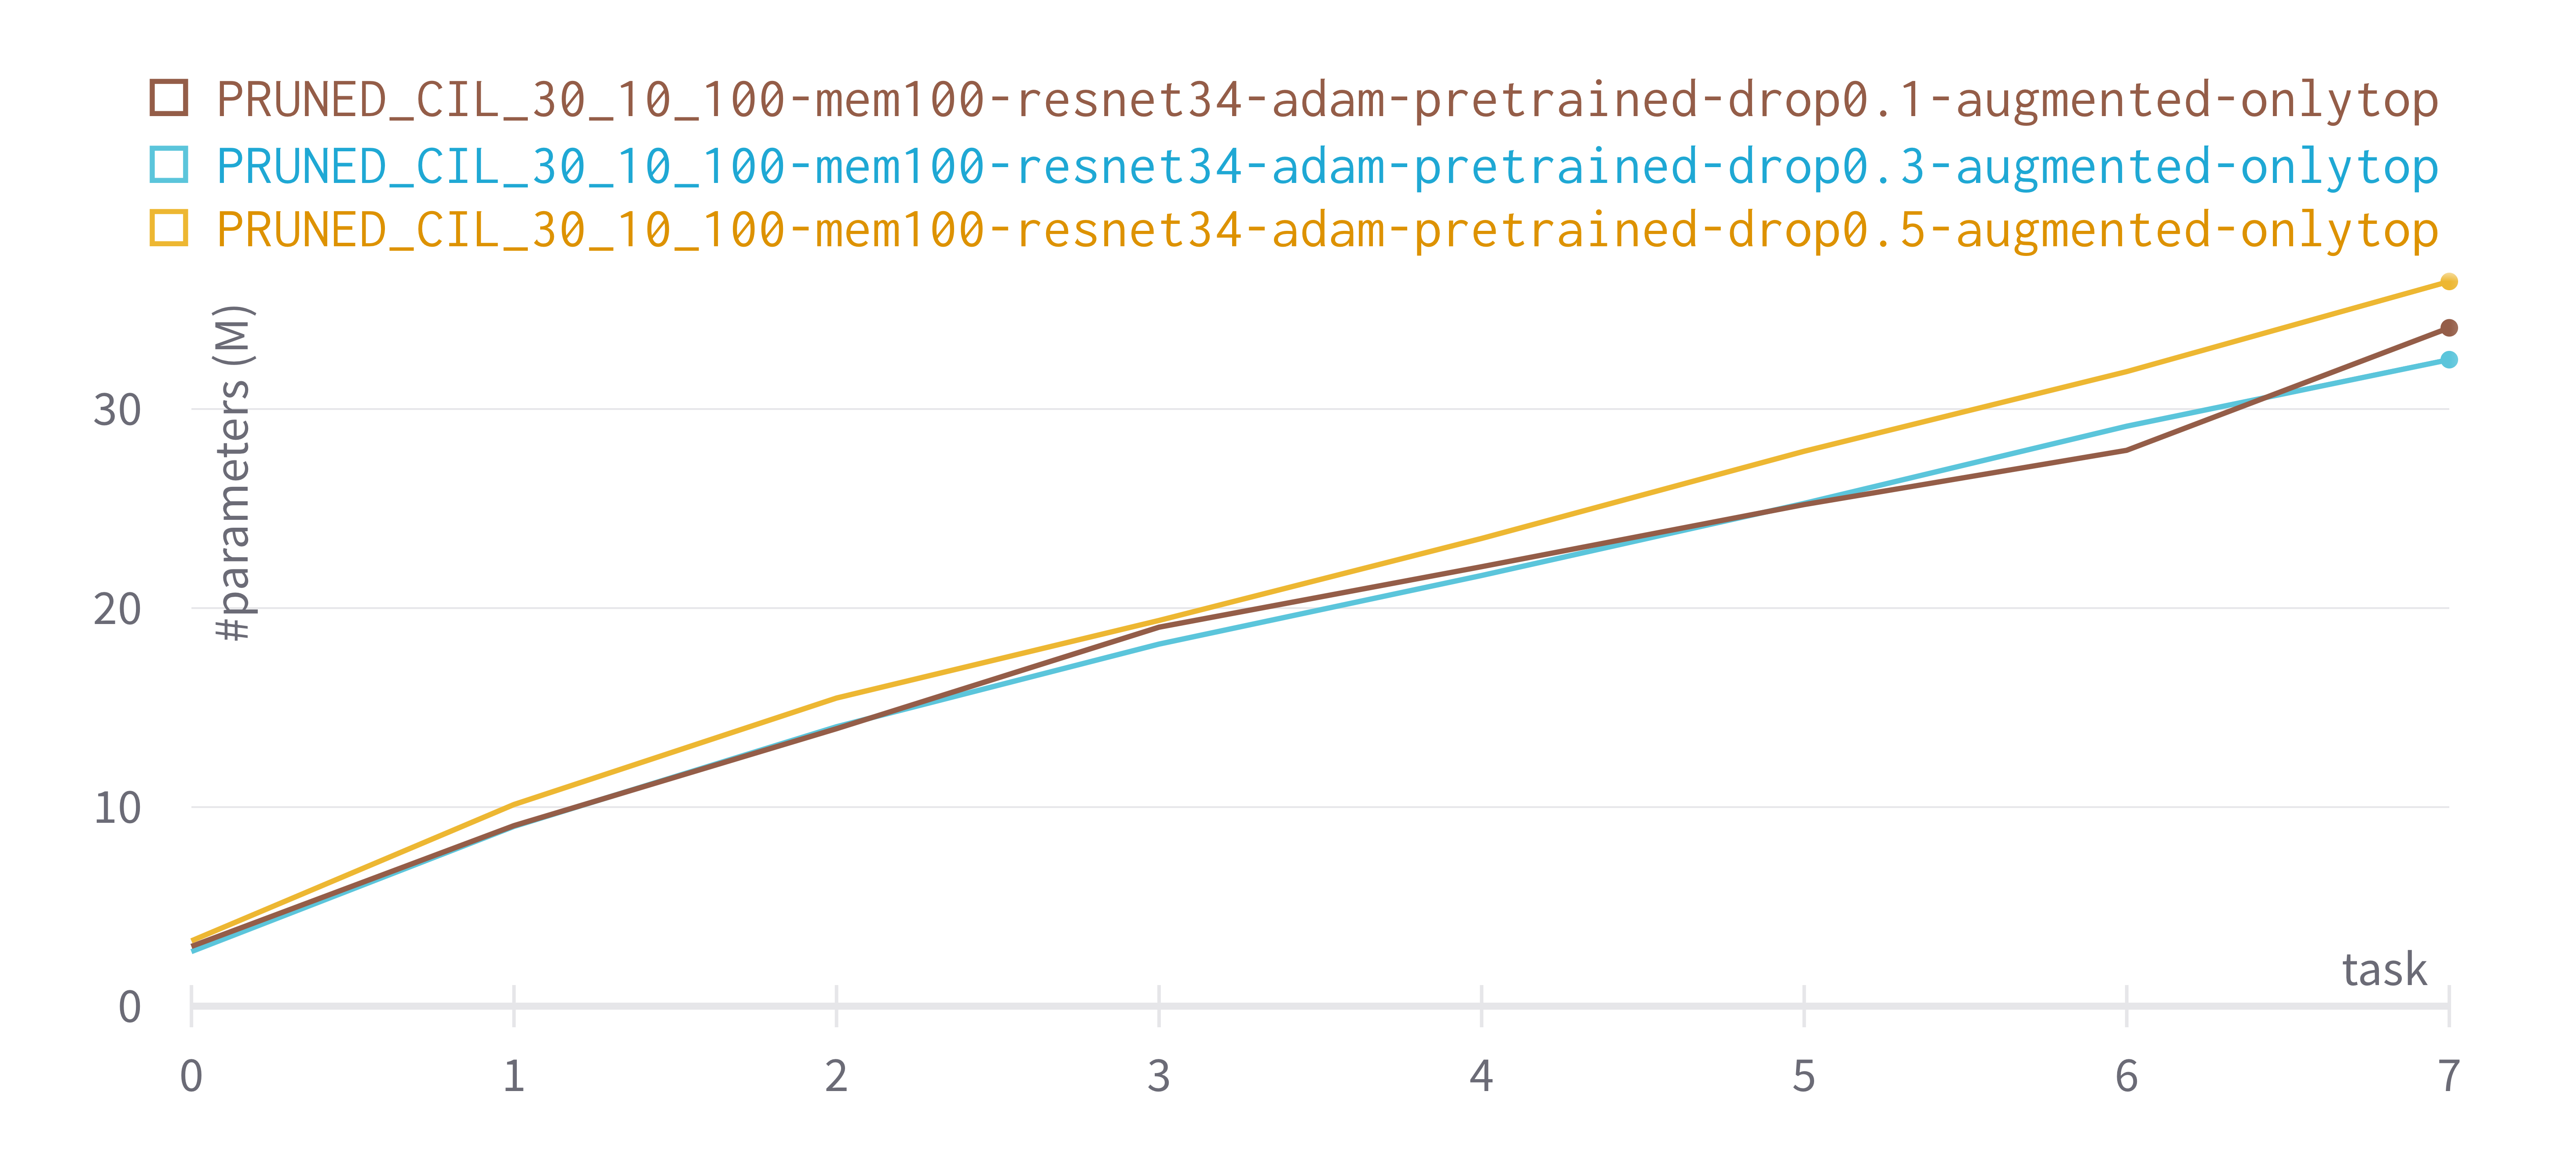
\includegraphics[width=1\linewidth]{images/exp/exp5-params.png}
        \captionof{figure}{Number of model parameters at each task using the pruning technique.}
        \label{fig:exp5-params}
    \end{minipage}
    \hfill
    \begin{minipage}[b]{0.49\linewidth}
        \centering
        \begin{tabular}{c|c}
            \hline
            \textbf{Model} &
            \textbf{\#Params} \\
            \textbf{name} &
            \textbf{(M)} \\
            \hline
            \hline
UNPRUNED-drop0.1&170\\
UNPRUNED-drop0.3&170\\
UNPRUNED-drop0.5&170\\
\hline
PRUNED-drop0.1&34.08\\
PRUNED-drop0.3&32.48\\
PRUNED-drop0.5&36.41\\
            \hline
        \end{tabular}
            \caption{Number of model parameters at task 7.}
            \label{table:exp5-params}
    \end{minipage}
\end{table}

Other interesting insights emerge by analyzing the training history of the models at task 0. The loss function of the DER algorithm (\autoref{eq:final_der_loss}) is defined as the sum of: the loss of the classifier, the loss of the auxiliary classifier and loss related to the pruning masks. In \autoref{fig:exp5-loss} we can see the classification loss (c), the sparsity loss (d) and the final loss (b) of the model for each training epoch at task 0. Initially, the loss (c) tends to decrease, but as the training epochs advance, the sparsity loss (d) increasingly limits the channels of the convolutional layers. This leads to a continuous decrease in parameters, but the classification (c) is affected considerably. The deterioration in performance can also be seen in the top-1 accuracy (a) on the validation set.


\begin{figure}[H]
	\centering
	\subfloat[\centering Top-1 accuracy]{{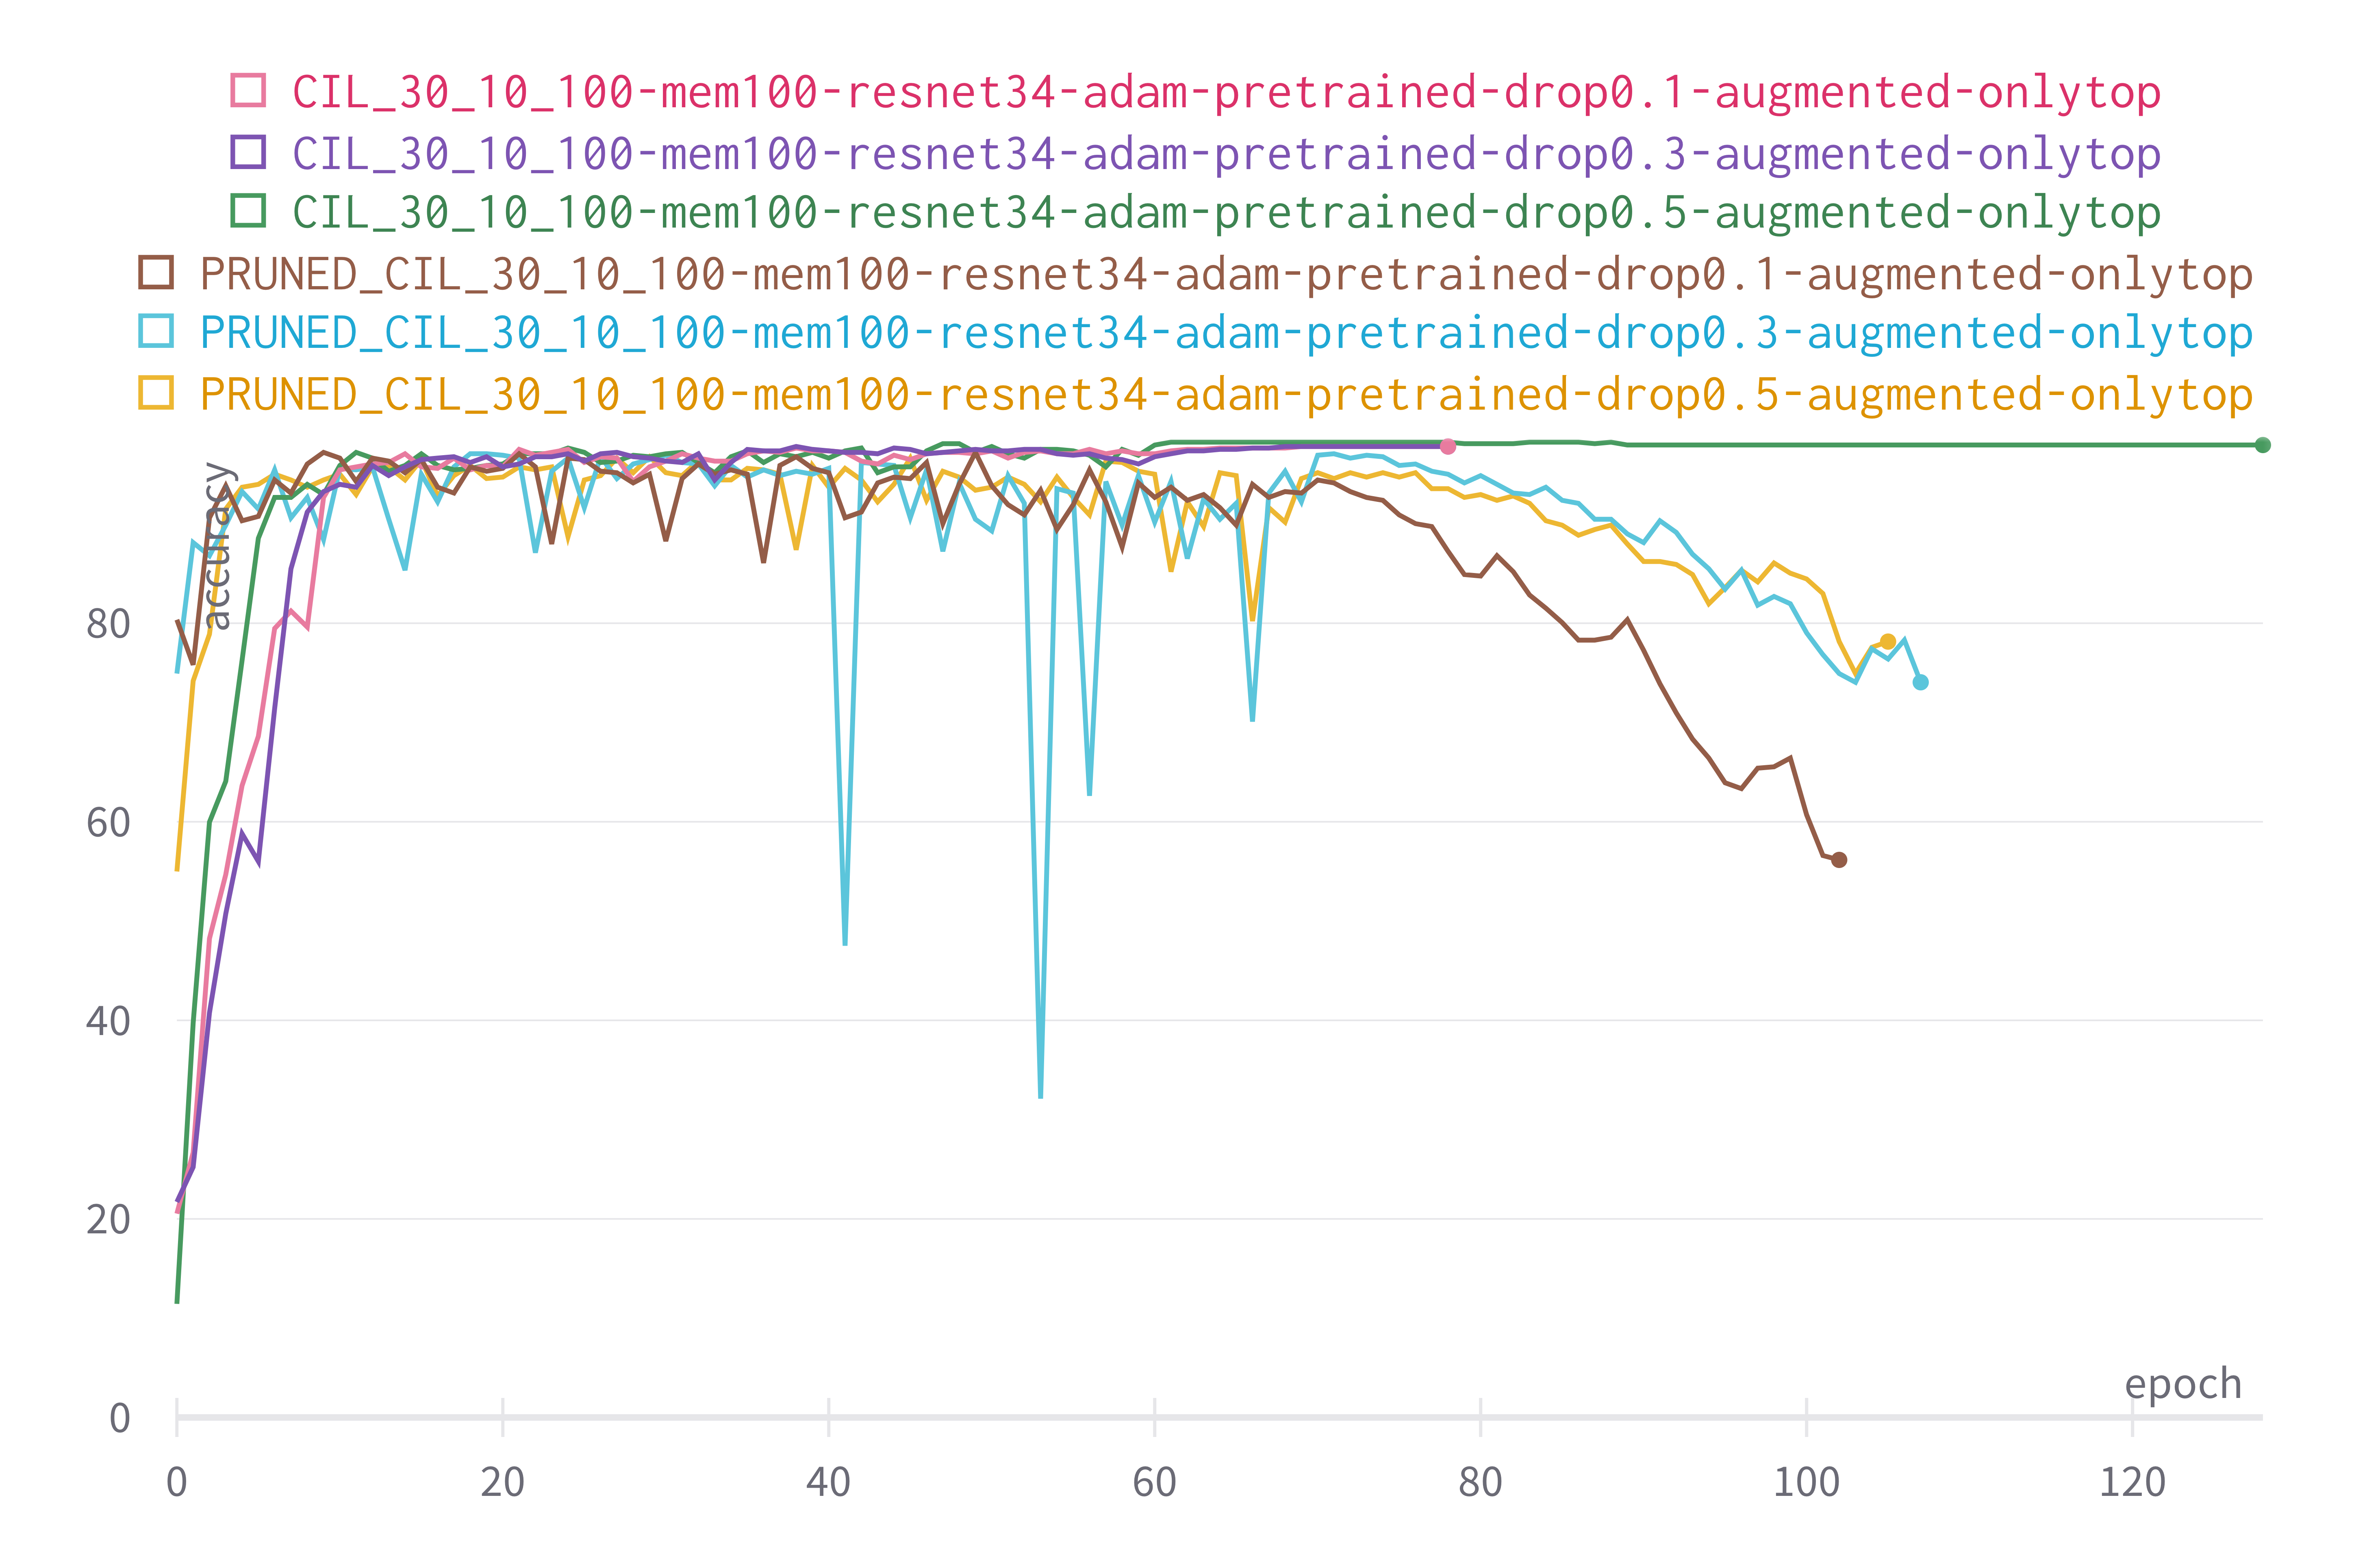
\includegraphics[width=0.50\textwidth]{images/exp/exp5-val_acc.png} }}%
    
	\subfloat[\centering Final loss]{{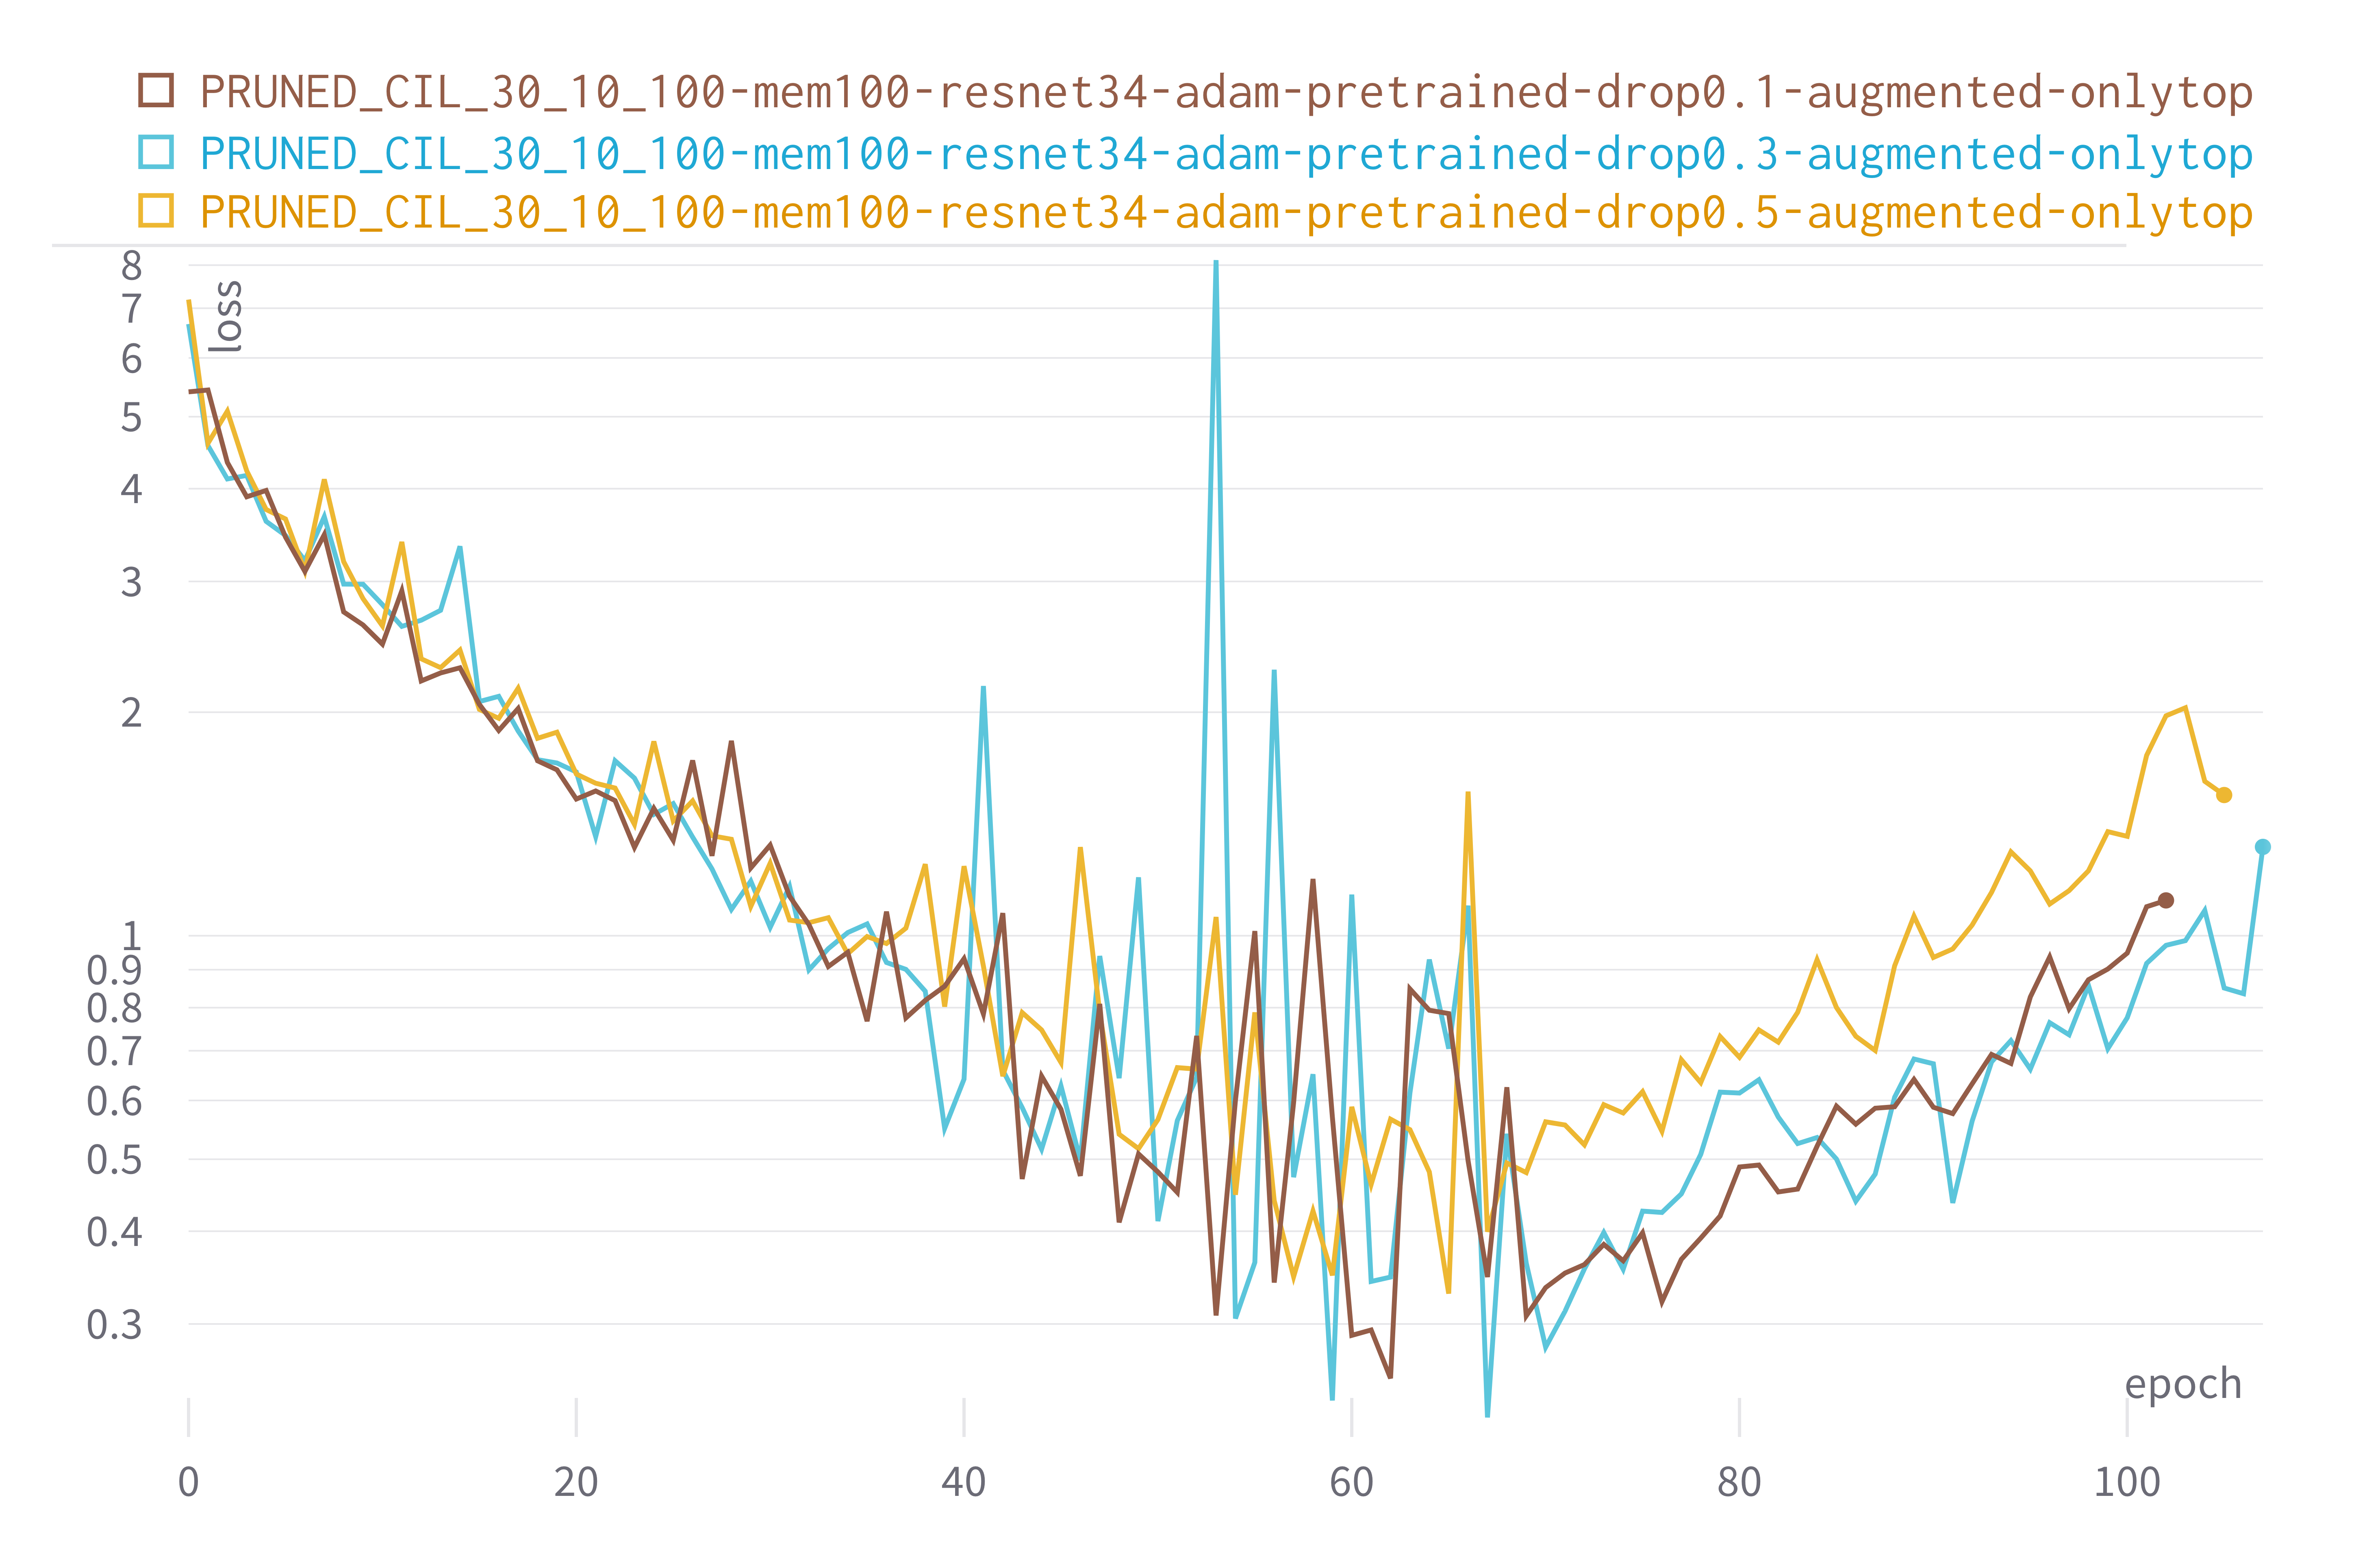
\includegraphics[width=0.50\textwidth]{images/exp/exp5-val_loss.png} }}%
    
	\subfloat[\centering Classification loss]{{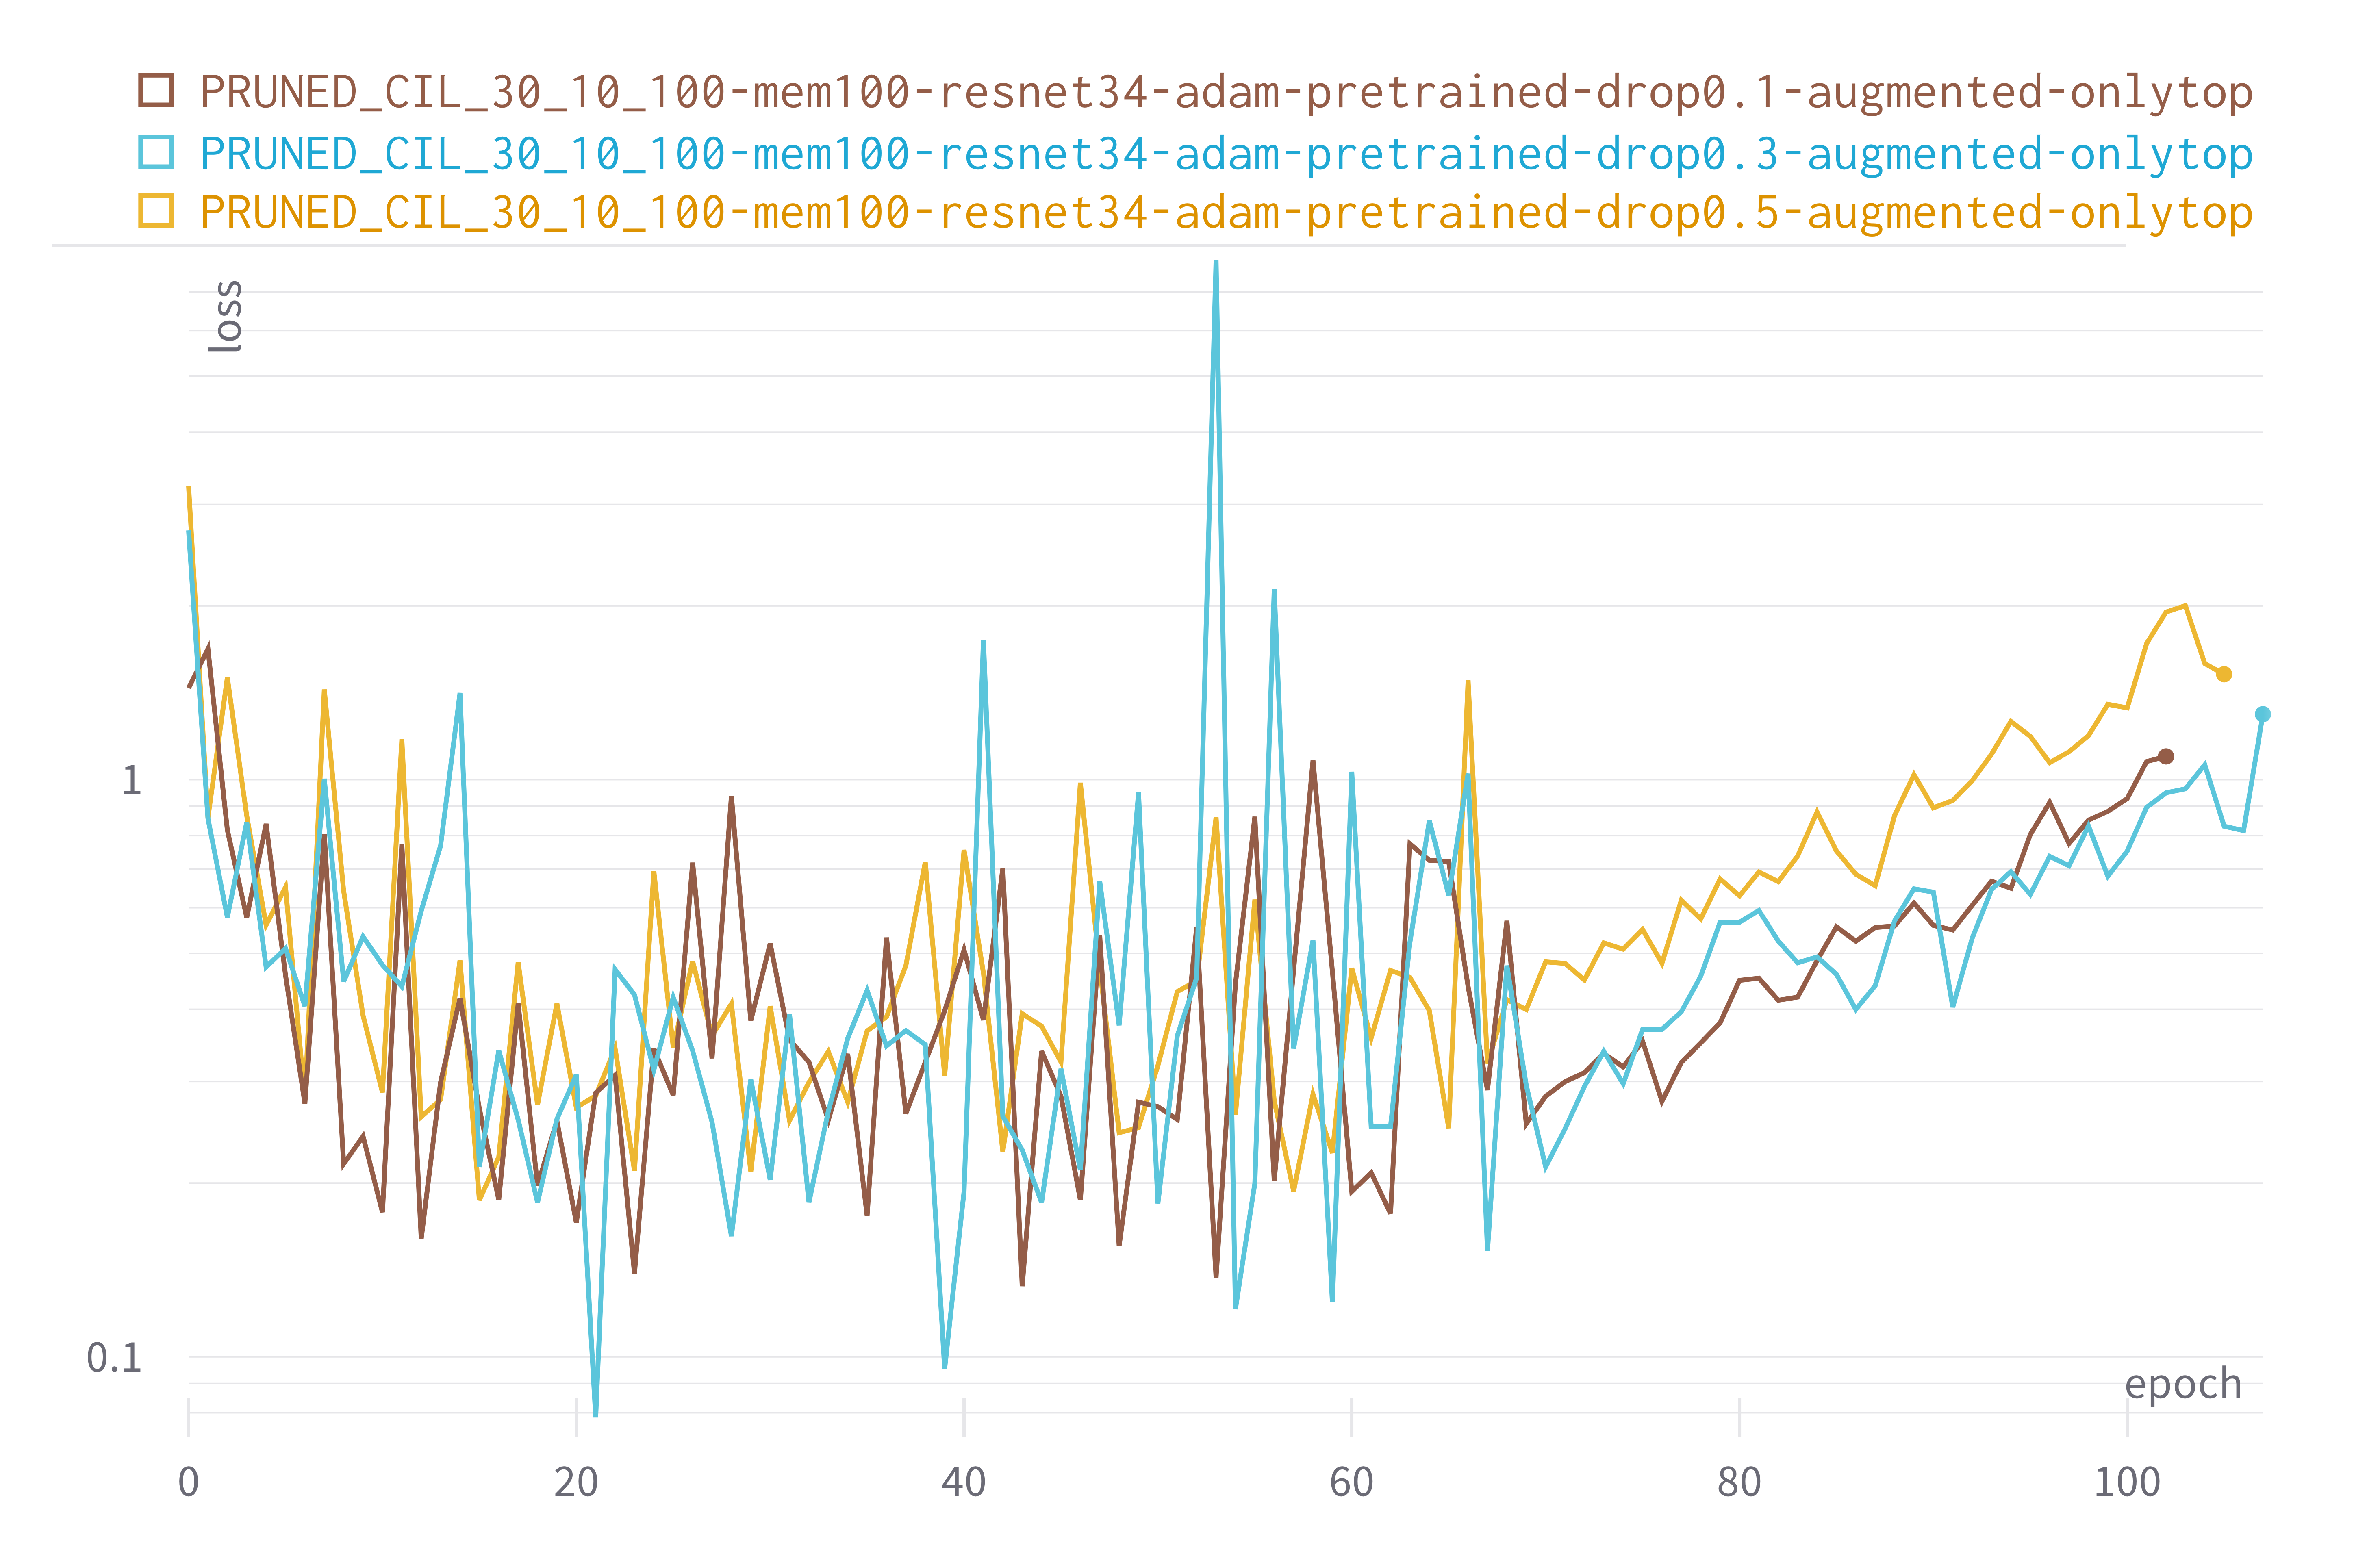
\includegraphics[width=0.50\textwidth]{images/exp/exp5-val_clf.png} }}%
    
	\subfloat[\centering Sparsity loss]{{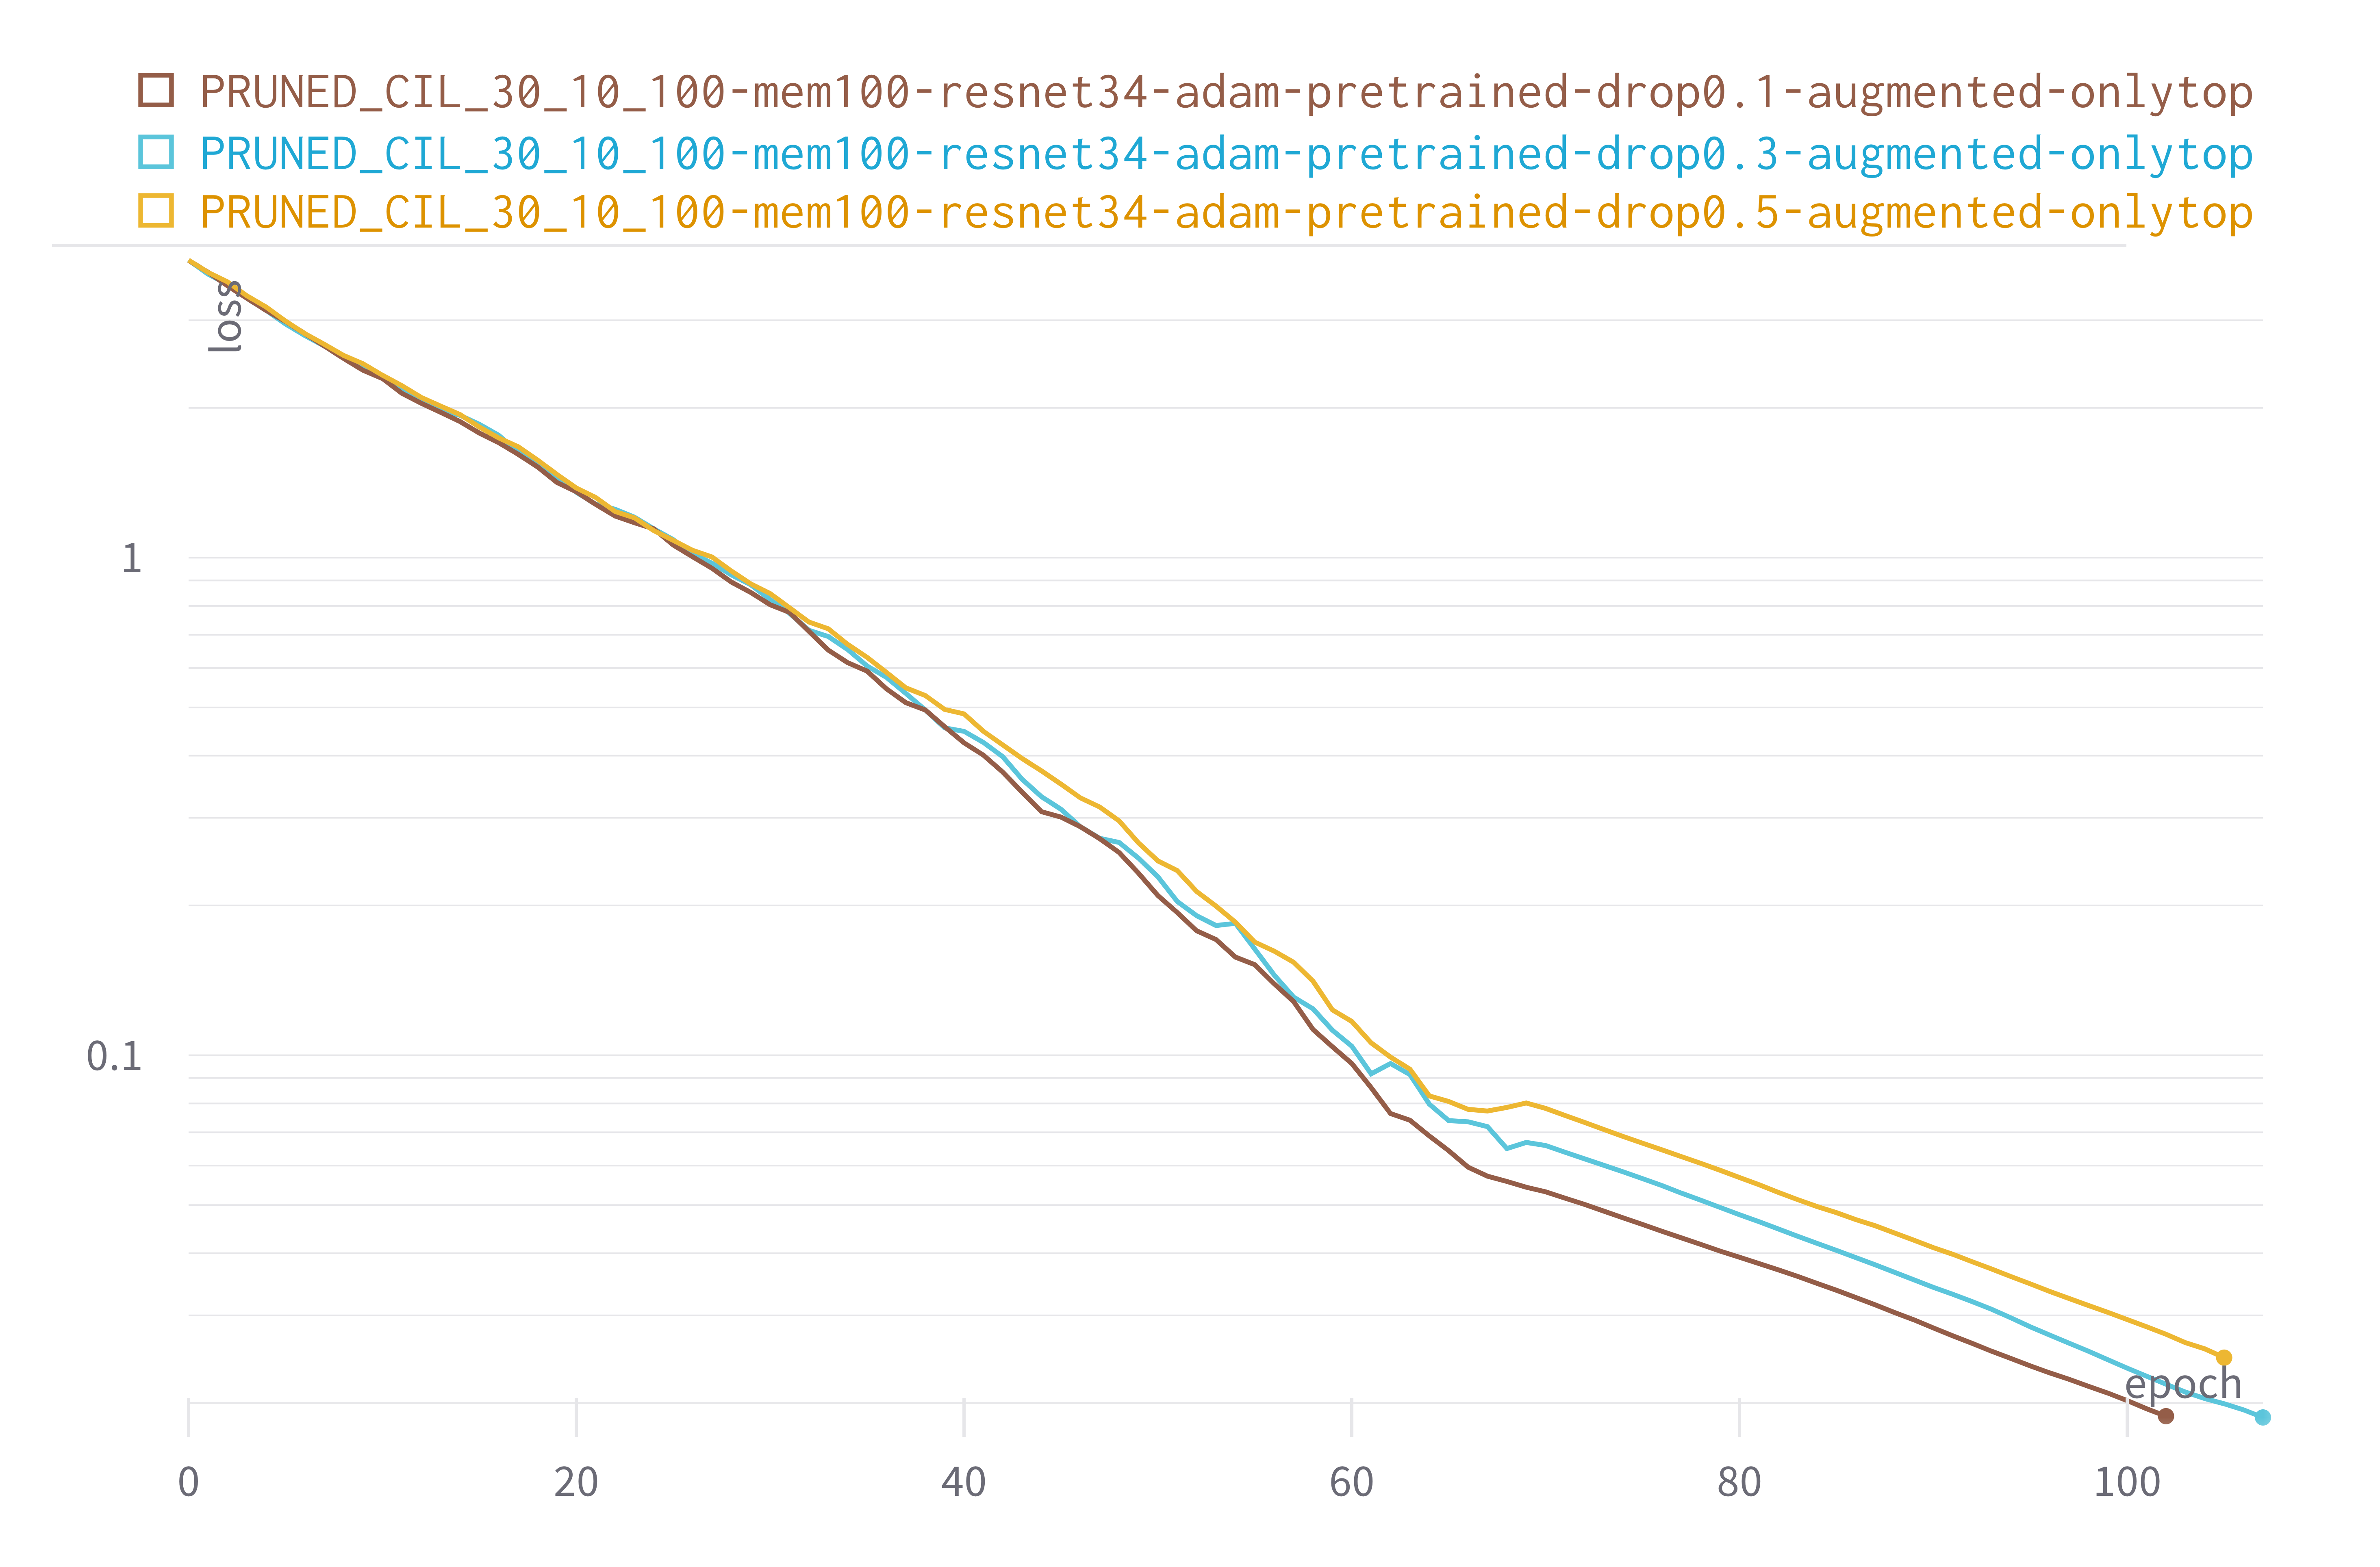
\includegraphics[width=0.50\textwidth]{images/exp/exp5-val_spars.png} }}%
	\caption{Training history of the pruned model on the validation set at task 0.}%
	\label{fig:exp5-loss}%
\end{figure}


\subsection{2993 Classes}
\label{sec:whole_dataset_clf}

The following experiments test the scalability capabilities of the model. In fact, in this section, models will be trained on 2993 classes, i.e. the entire dataset.

\subsubsection{Varying the memory size}
Another important factor for testing the scalability of the model is the number of stored examples for old classes. Indeed, when many classes are introduced, it is necessary to limit the memory used to save old examples.
In this first section, the models are trained by varying the size of the memory used by the models to store examples of the old classes. The memory size is tested using: 50, 20 and 10 examples.

Regarding the other specifications of the model, it is trained according to the best results obtained previously with the experiments on 100 classes. Thus, the architecture of each feature extractor is ResNet-34 pretrained on ImageNet, the optimizer is Adam, regularization with a dropout layer is used as well as data augmentation, but initially no pruning is performed.

The results of the experiments are shown in \autoref{fig:exp6} and \autoref{table:exp6}.
As we can see, the models scale fairly well over the entire dataset, as a comparison of the setup of 100 classes shown in \autoref{table:exp5}, the drop in performance is only about 8\%, even though the examples stored in the setup of 2993 classes are 1/10 than before. As expected, the more samples stored for incremental learning iterations, the better the overall accuracy. The total number of examples stored by each model at task 8 is shown in \autoref{table:exp6-memsize}.

\begin{table}[H]
    \centering
    \centerline{
    \begin{tabular}{c|c|c|c|c}
        \hline
        \textbf{Model} &
        \textbf{Dropout} &
        \textbf{Mem.} &
        \textbf{Top-1} & 
        \textbf{Top-5} \\
        \textbf{name} &
        \textbf{rate} &
        \textbf{size} &
        \textbf{acc. (\%)} & 
        \textbf{acc. (\%)} \\
        \hline
        \hline
CIL\_2993-mem10-drop0.5-adam&0.1&10&87.2&92.19\\
CIL\_2993-mem20-drop0.5-adam&0.1&20&88.47&92.58\\
CIL\_2993-mem50-drop0.5-adam&0.1&50&\textbf{89.22}&\textbf{92.97}\\
        \hline
    \end{tabular}}
    \caption{Performance of the models at each incremental task trained on the entire dataset using different dimensions of memory size. Top-1 accuracy at task 8.}
    \label{table:exp6}
\end{table}


\begin{table}[H]
    \centering
    \begin{tabular}{c|c|c}
        \hline
        \textbf{Model} &
        \textbf{Mem.} &
        \textbf{\# Total saved} \\
        \textbf{name} &
        \textbf{per class} &
        \textbf{examples (K)} \\
        \hline
        \hline
CIL\_2993-mem10-drop0.5-adam&10&102\\
CIL\_2993-mem20-drop0.5-adam&20&53\\
CIL\_2993-mem50-drop0.5-adam&50&29\\
        \hline
    \end{tabular}
    \caption{Number of total examples stored by each model at task 8.}
    \label{table:exp6-memsize}
\end{table}


\begin{figure}[H]
	\centering
	\subfloat[\centering Top-1 accuracy]{{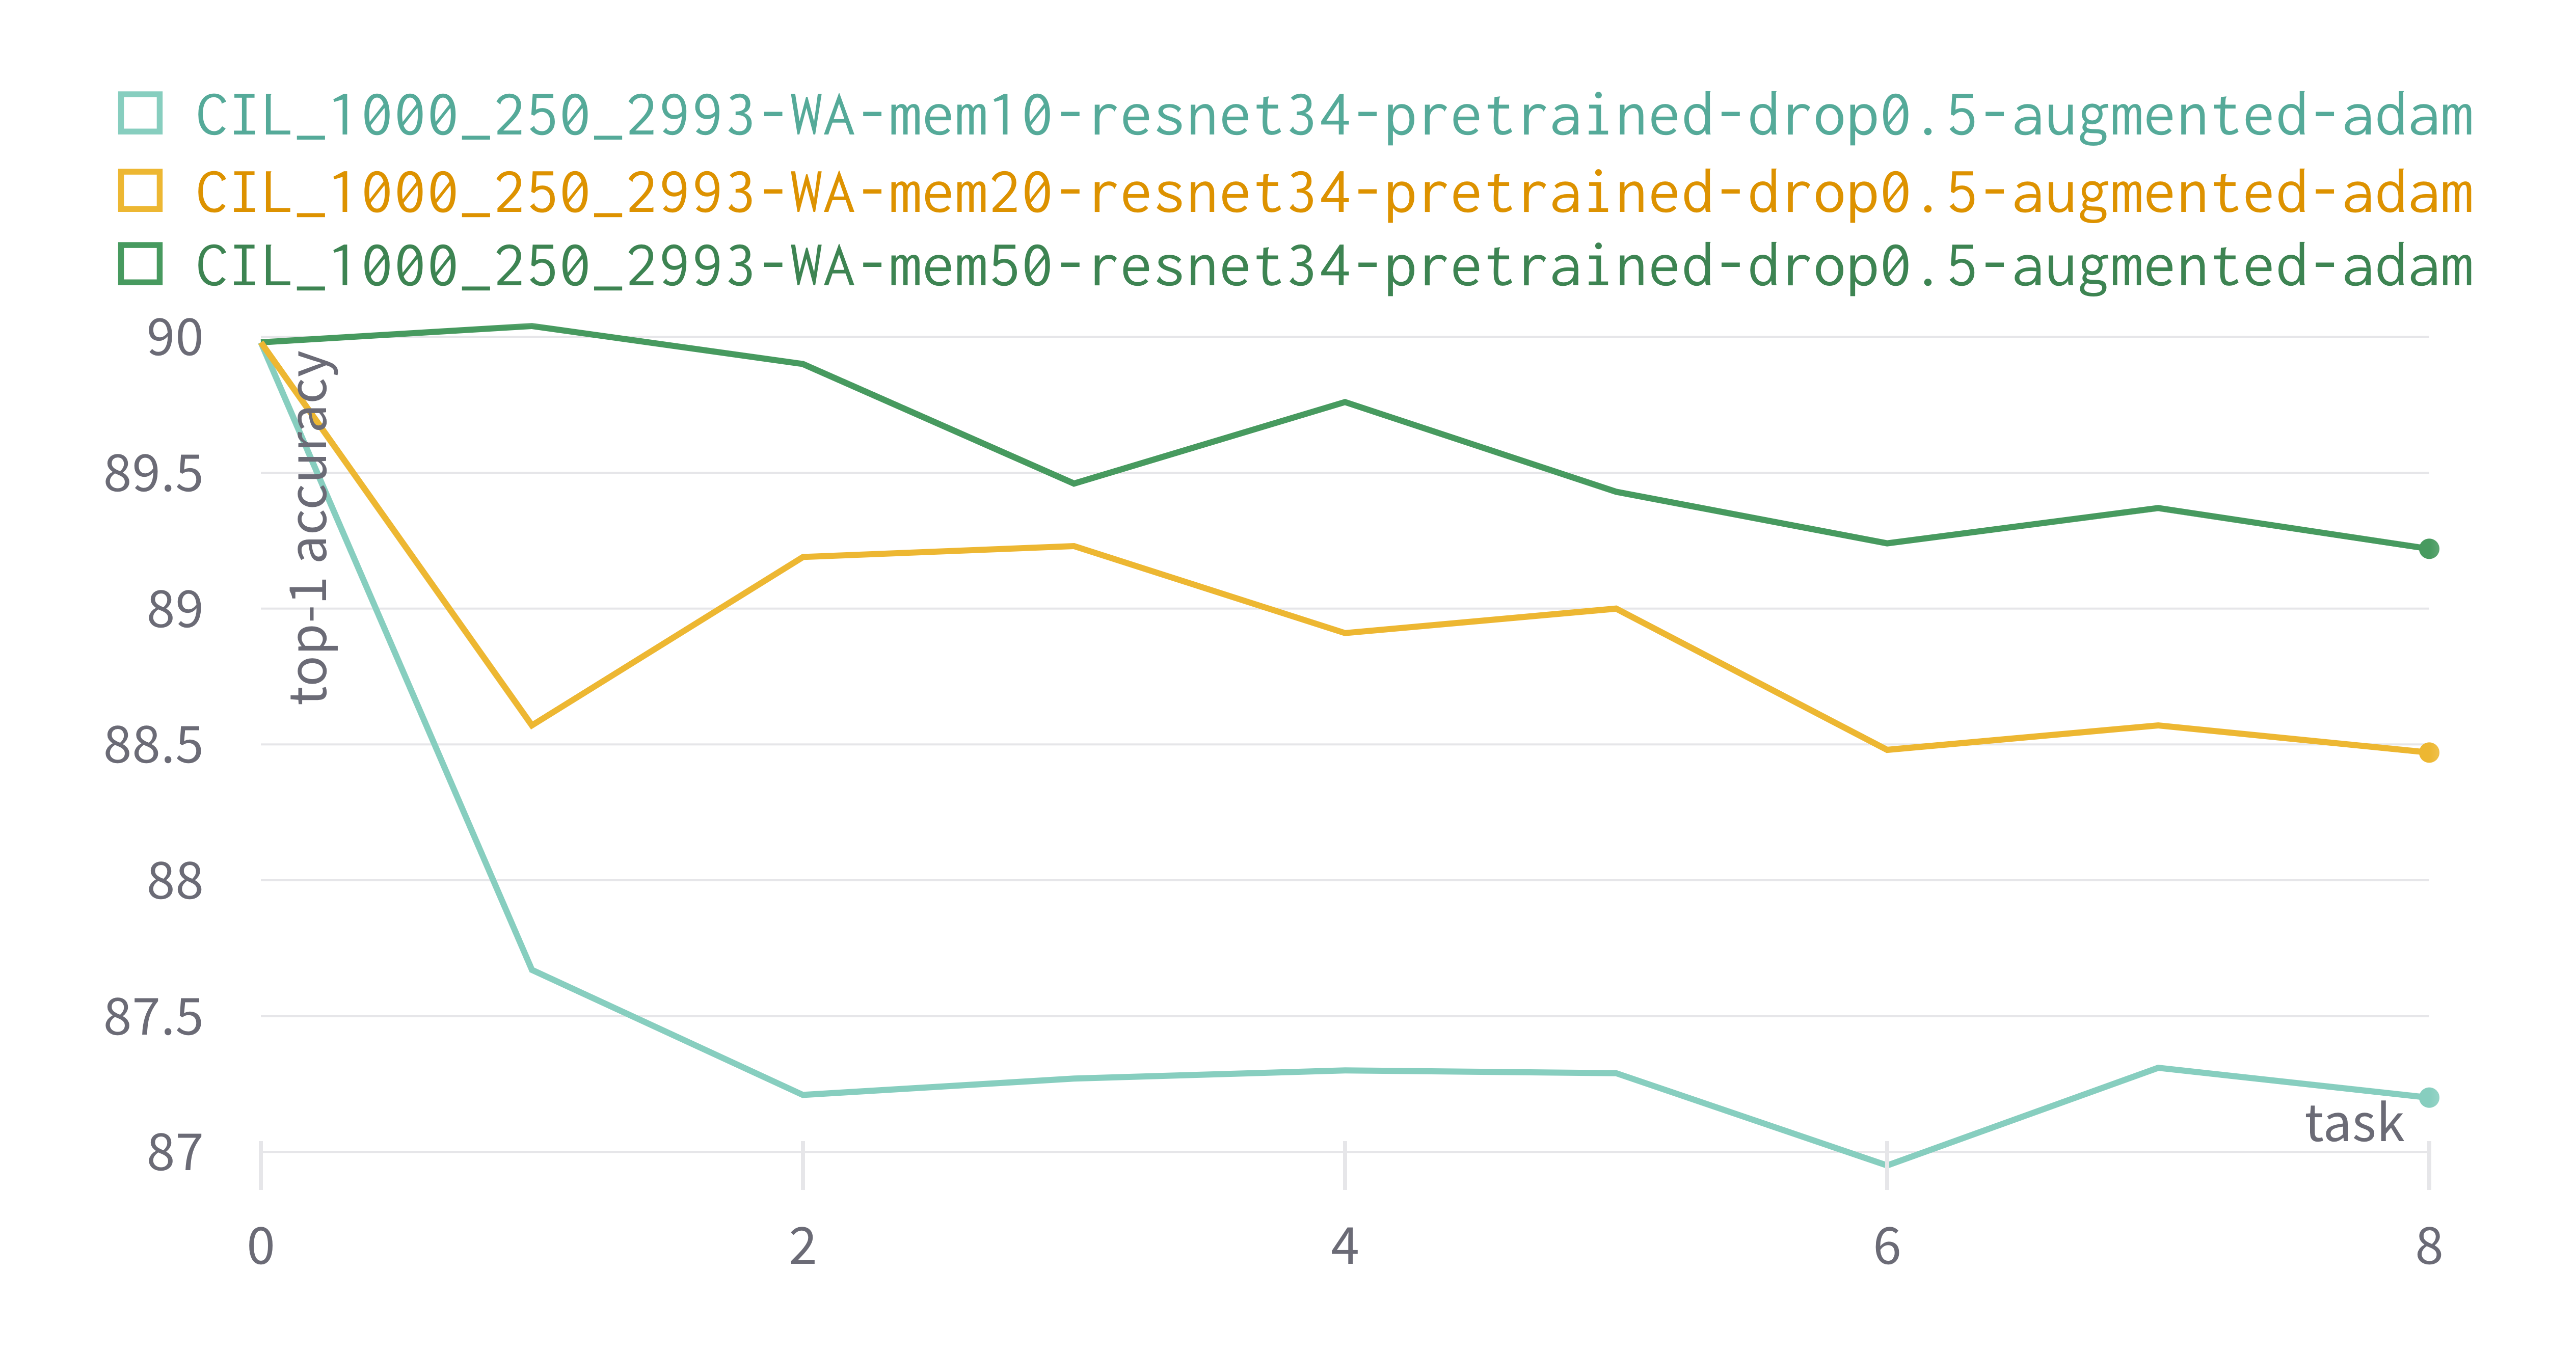
\includegraphics[width=0.80\textwidth]{images/exp/exp6-top1.png} }}%
    \qquad
	\subfloat[\centering Top-5 accuracy]{{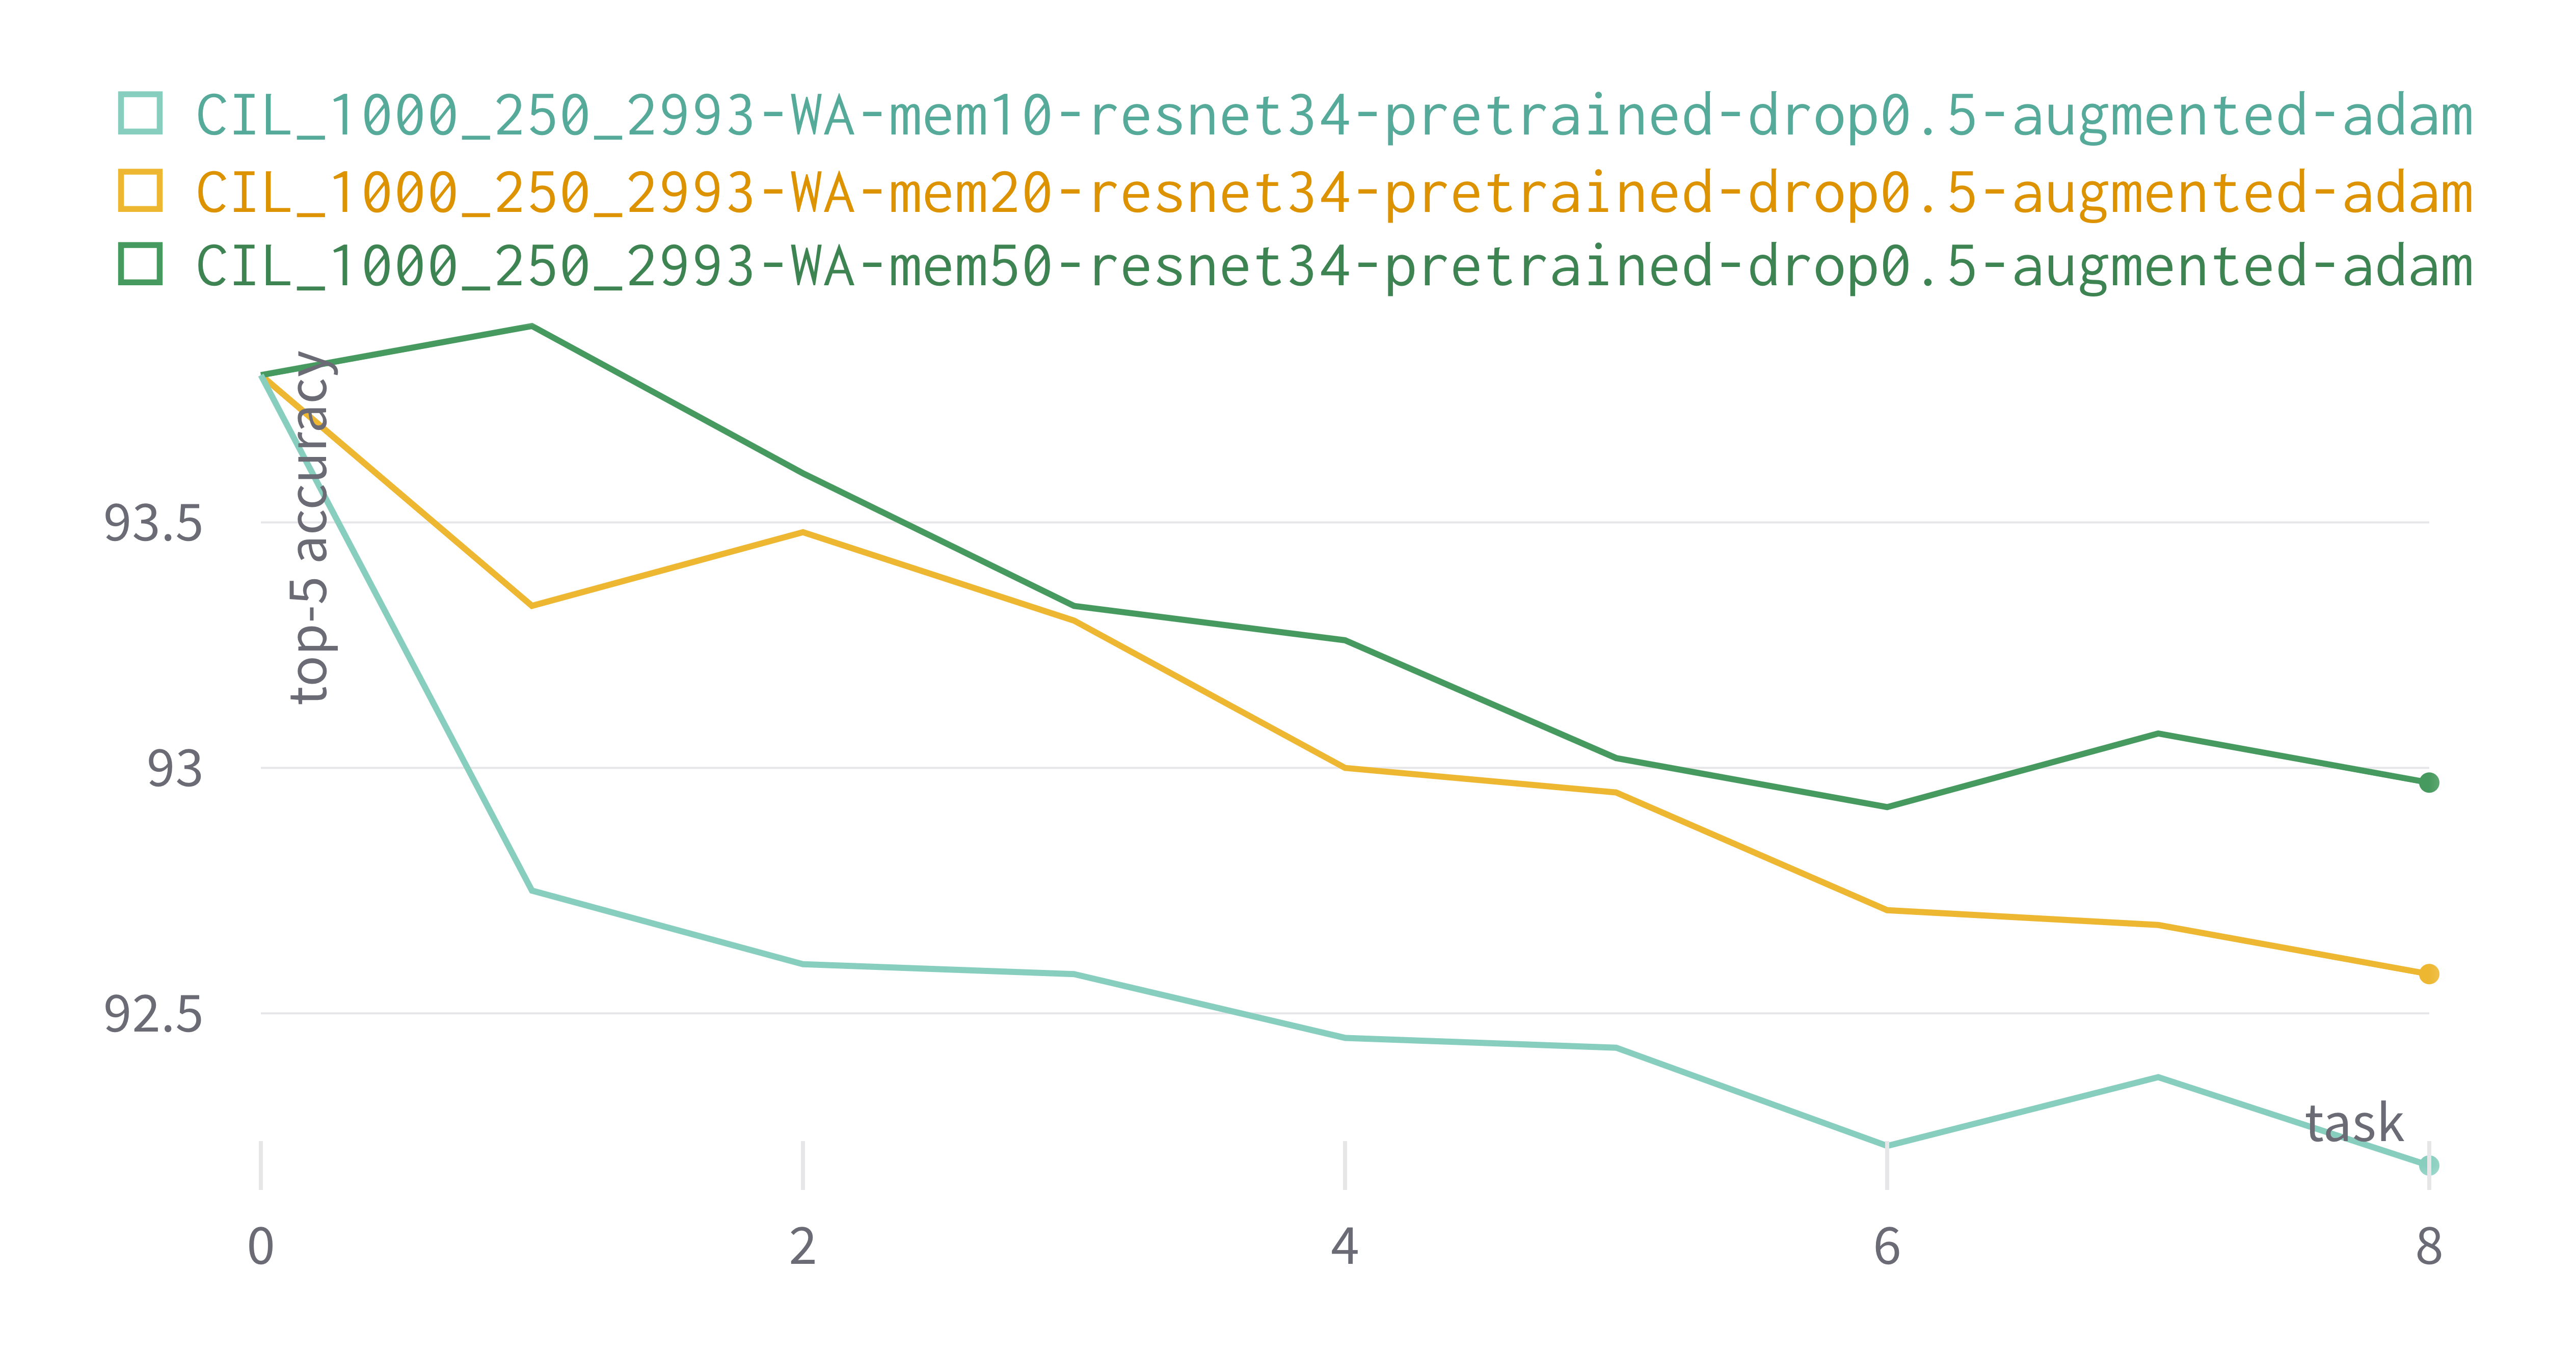
\includegraphics[width=0.80\textwidth]{images/exp/exp6-top5.png} }}%
	\caption{Performance of the models at each incremental task trained on the entire dataset using different dimensions of memory size.}%
	\label{fig:exp6}%
\end{figure}

\newpage

\subsubsection{Type 3 baseline (2993 classes)}
As in the case of 100 classes, the performance of the CIL models is compared with the type 3 baseline (see \autoref{sec:method-baseline3}). For this purpose, the baseline is trained considering the same dataset used to train the models in the previous section.
Note that in the case of the baseline, there is no need to use a memory for the old classes since the incremental learning setup does not hold.
 
The comparison of top-1 accuracy between CIL models and baselines is shown in \autoref{table:baseline3-2993}.
Osservazioni\todo{Osservazioni}


\begin{table}[H]
    \centering
    \centerline{
    \begin{tabular}{c|c|c|c}
        \hline
        \textbf{Model} &
        \textbf{Dropout} &
        \textbf{Mem.} &
        \textbf{Top-1}\\
        \textbf{name} &
        \textbf{rate} &
        \textbf{size} &
        \textbf{acc. (\%)} \\
        \hline
\hline
CIL\_2993-mem10-drop0.5-adam&0.1&10&87.2\\
CIL\_2993-mem20-drop0.5-adam&0.1&20&88.47\\
CIL\_2993-mem50-drop0.5-adam&0.1&50&89.22\\
\hline\
BASELINE\_3-2993classes-drop0.1&0.1&-&-\\
BASELINE\_3-2993classes-drop0.3&0.3&-&-\\
BASELINE\_3-2993classes-drop0.5&0.5&-&-\\
\hline 
    \end{tabular}}
    \caption{Top-1 accuracy of the CIL model and the type 3 baseline consider all the 100 classes of the test set.}
    \label{table:baseline3-2993}
\end{table}

\newpage

\subsubsection{Pruning (2993 classes)}
\label{sec:pruning-entire}
Similarly to the setup with 100 classes, the pruning strategy is tested for models trained on the entire dataset. As we can see from \autoref{fig:exp7} and \autoref{table:exp7}, when using the pruning in combination to the Weight Aligning (WA), the performance drops dramatically. Therefore, only for models using pruning, WA is disabled.

In contrast to the experiments on 100 classes, now pruning results in poor performance, in fact the drop in accuracy is considerable compared to those models without pruning. Even considering the case using 50 samples for the pruning model, performance deteriorates by almost 20\%.

Regarding the number of parameters, even in the setup with 2993 classes the model is reduced in size considerably. As we can see from \autoref{table:exp7-params}, however, the pruning factor corresponds to approximately 3x compared to the 5x achieved in the previous setup.

In conclusion, the pruning strategy is not effective in the case of models trained on the entire dataset. For this reason, the KD is used and the result of the experiments is shown in \autoref{sec:exp-kd}.

\begin{table}[H]
    \centering
    \begin{tabular}{c|c|c|c|c|c}
        \hline
        \textbf{Model} &
        \textbf{Mem.} &
        \textbf{WA} &
        \textbf{Pruning} &
        \textbf{Top-1} & 
        \textbf{Top-5} \\
        \textbf{name} &
        \textbf{size} &
        &
        &
        \textbf{acc. (\%)} & 
        \textbf{acc. (\%)} \\
        \hline
        \hline
UNPRUNED-WA-mem10-drop0.5&10&yes&no&87.2&92.19\\
UNPRUNED-WA-mem20-drop0.5&20&yes&no&88.47&92.58\\
UNPRUNED-WA-mem50-drop0.5&50&yes&no&\textbf{89.22}&\textbf{92.97}\\
\hline
PRUNED-noWA-mem10-drop0.3&10&no&yes&51.69&62.56\\
PRUNED-noWA-mem20-drop0.3&20&no&yes&63.2&73.97\\
PRUNED-noWA-mem50-drop0.3&50&no&yes&70.37&81.85\\
\hline
PRUNED-WA-mem10-drop0.3&50&no&yes&7.6&10.67\\
\hline
\end{tabular}
\caption{Performance comparison between the pruned and un-pruned models. Top-1 accuracy at task 8.}
    \label{table:exp7}
\end{table}


\begin{table}[H]
    \centering
    \begin{tabular}{c|c}
        \hline
        \textbf{Model} &
        \textbf{\#Params} \\
        \textbf{name} &
        \textbf{(M)} \\
        \hline
        \hline
UNPRUNED-CIL\_2993-WA-mem10-drop0.5&205\\
UNPRUNED-CIL\_2993-WA-mem20-drop0.5&205\\
UNPRUNED-CIL\_2993-WA-mem50-drop0.5&205\\
\hline
PRUNED-CIL\_2993-noWA-mem10-drop0.3&68.79\\
PRUNED-CIL\_2993-noWA-mem20-drop0.3&71.66\\
PRUNED-CIL\_2993-noWA-mem50-drop0.3&68.33\\
\hline
PRUNED-CIL\_2993-WA-mem10-drop0.3&70.69\\
        \hline
    \end{tabular}
	\caption{Number of model parameters at task 8.}%
    \label{table:exp7-params}
\end{table}

\begin{figure}[H]
	\centering
	\subfloat[\centering Top-1 accuracy]{{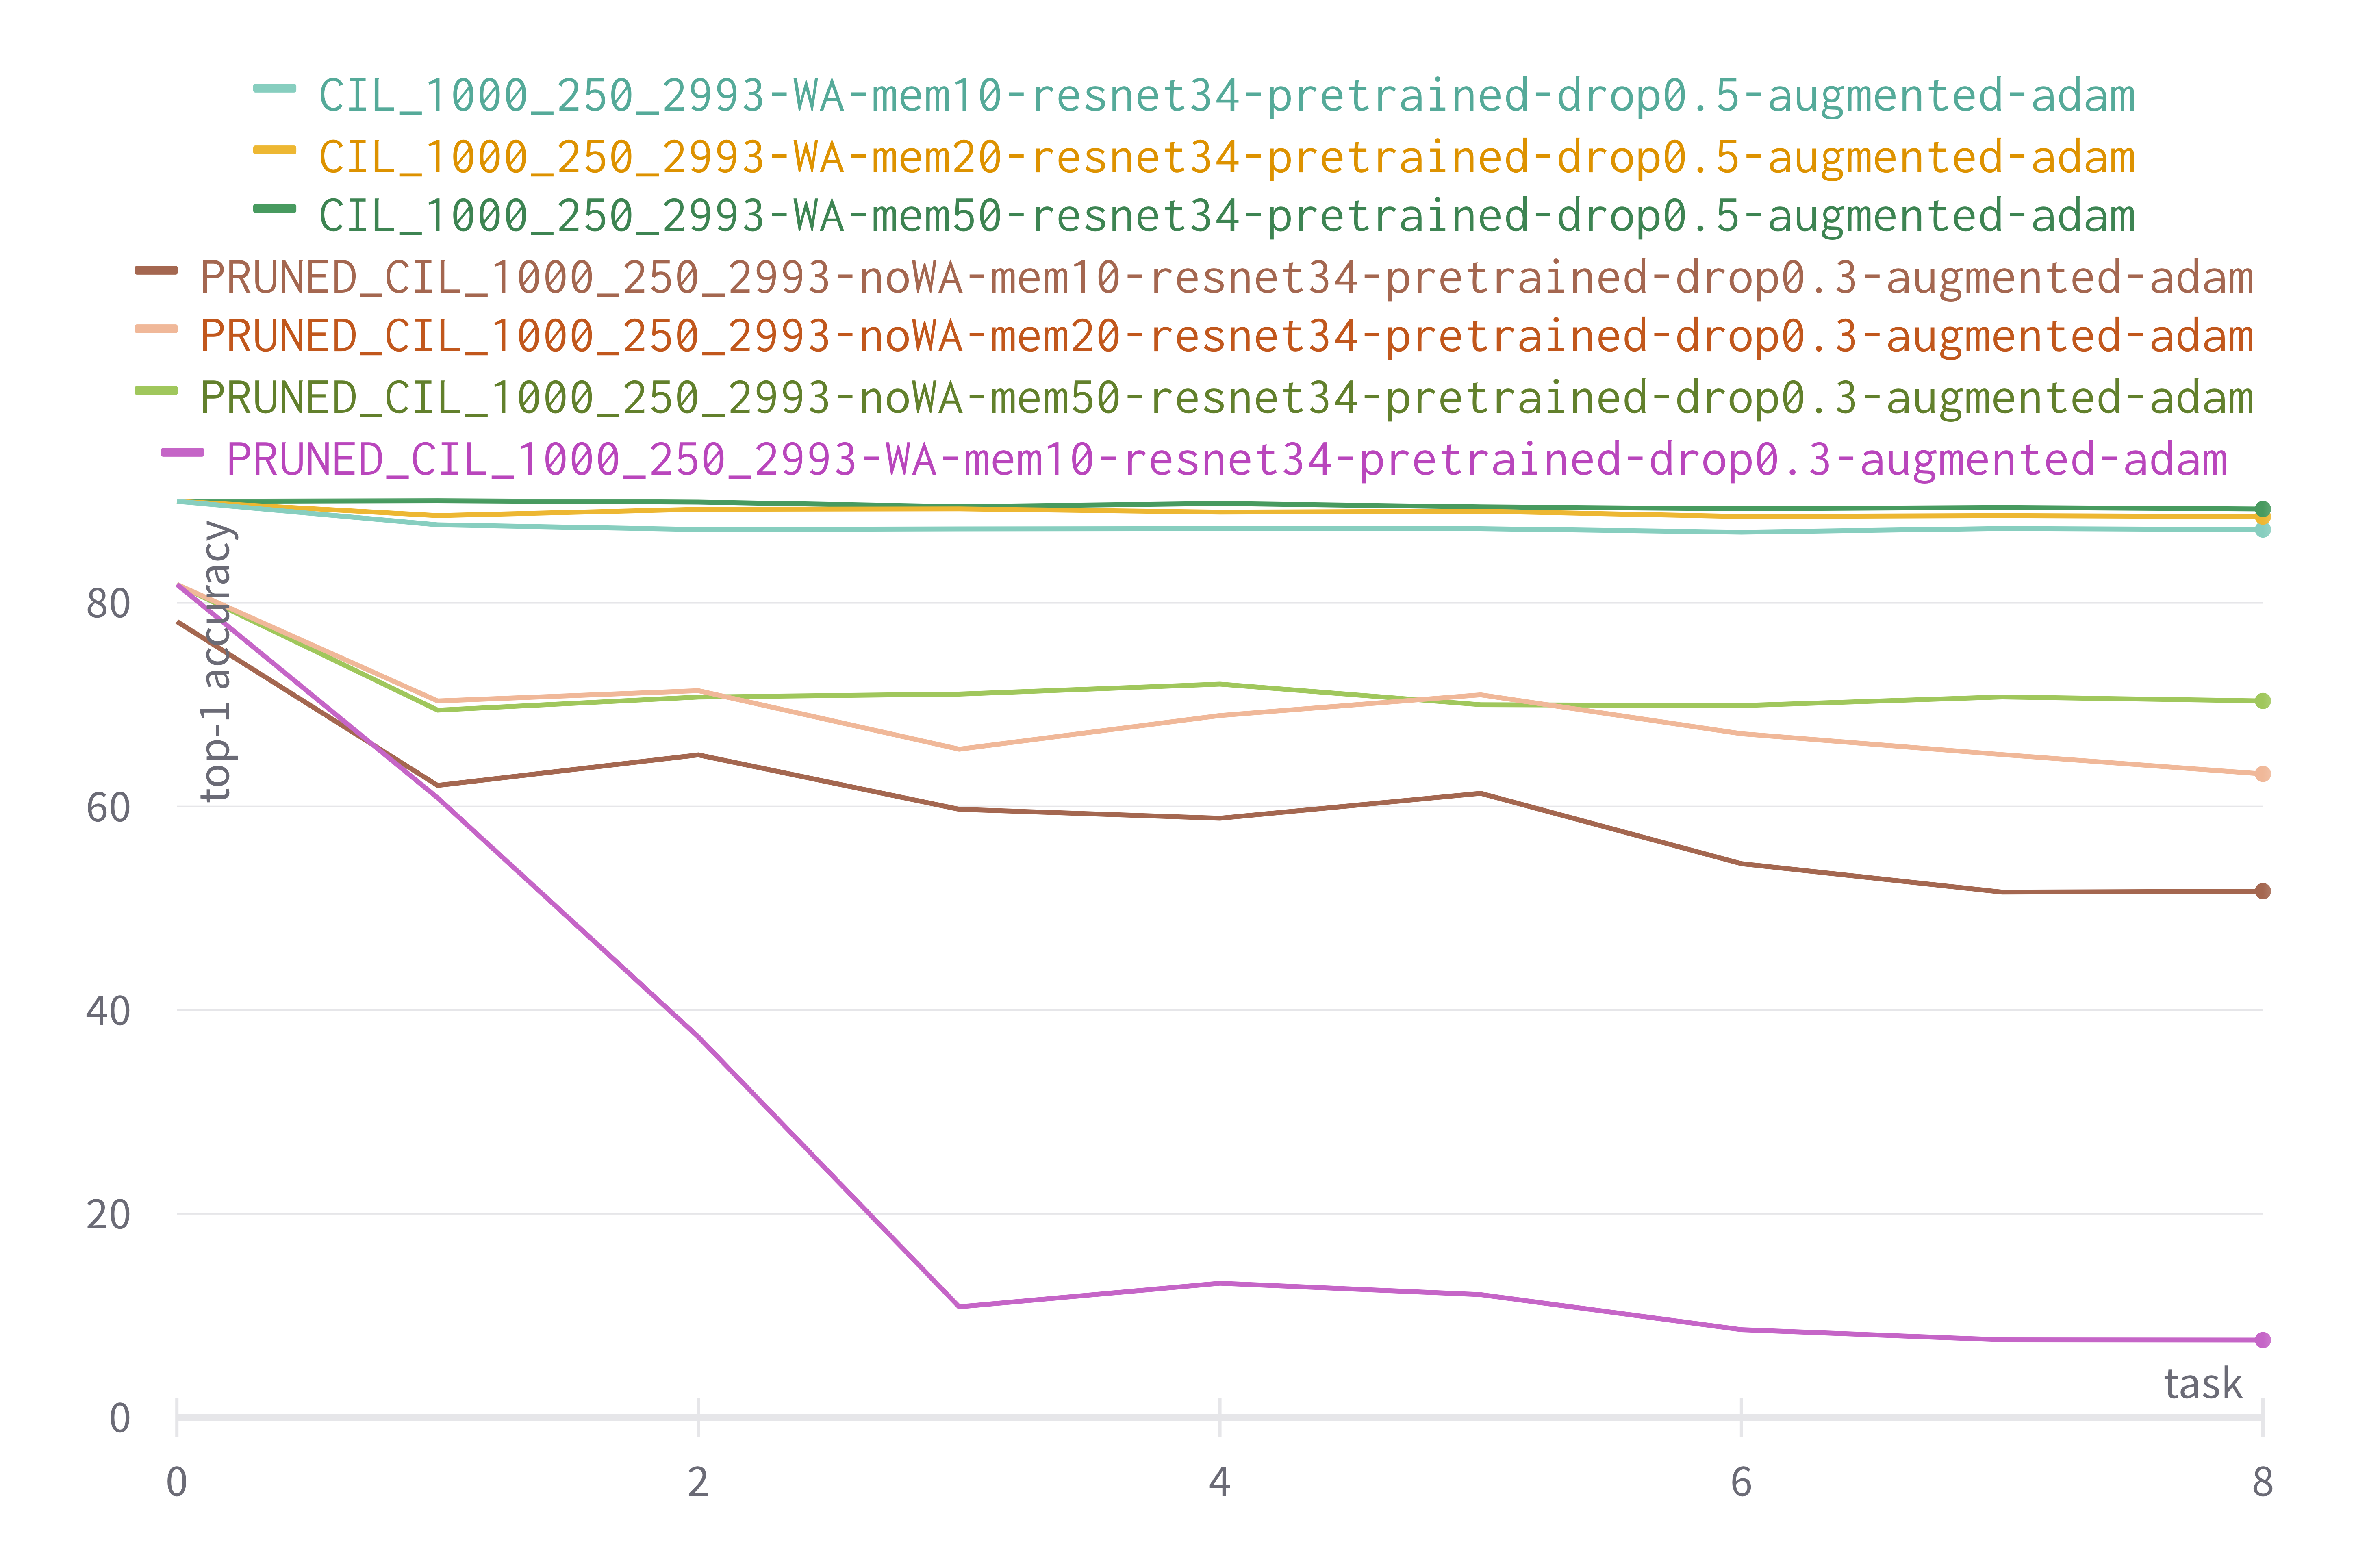
\includegraphics[width=0.80\textwidth]{images/exp/exp7-top1.png} }}%
    \qquad
	\subfloat[\centering Top-5 accuracy]{{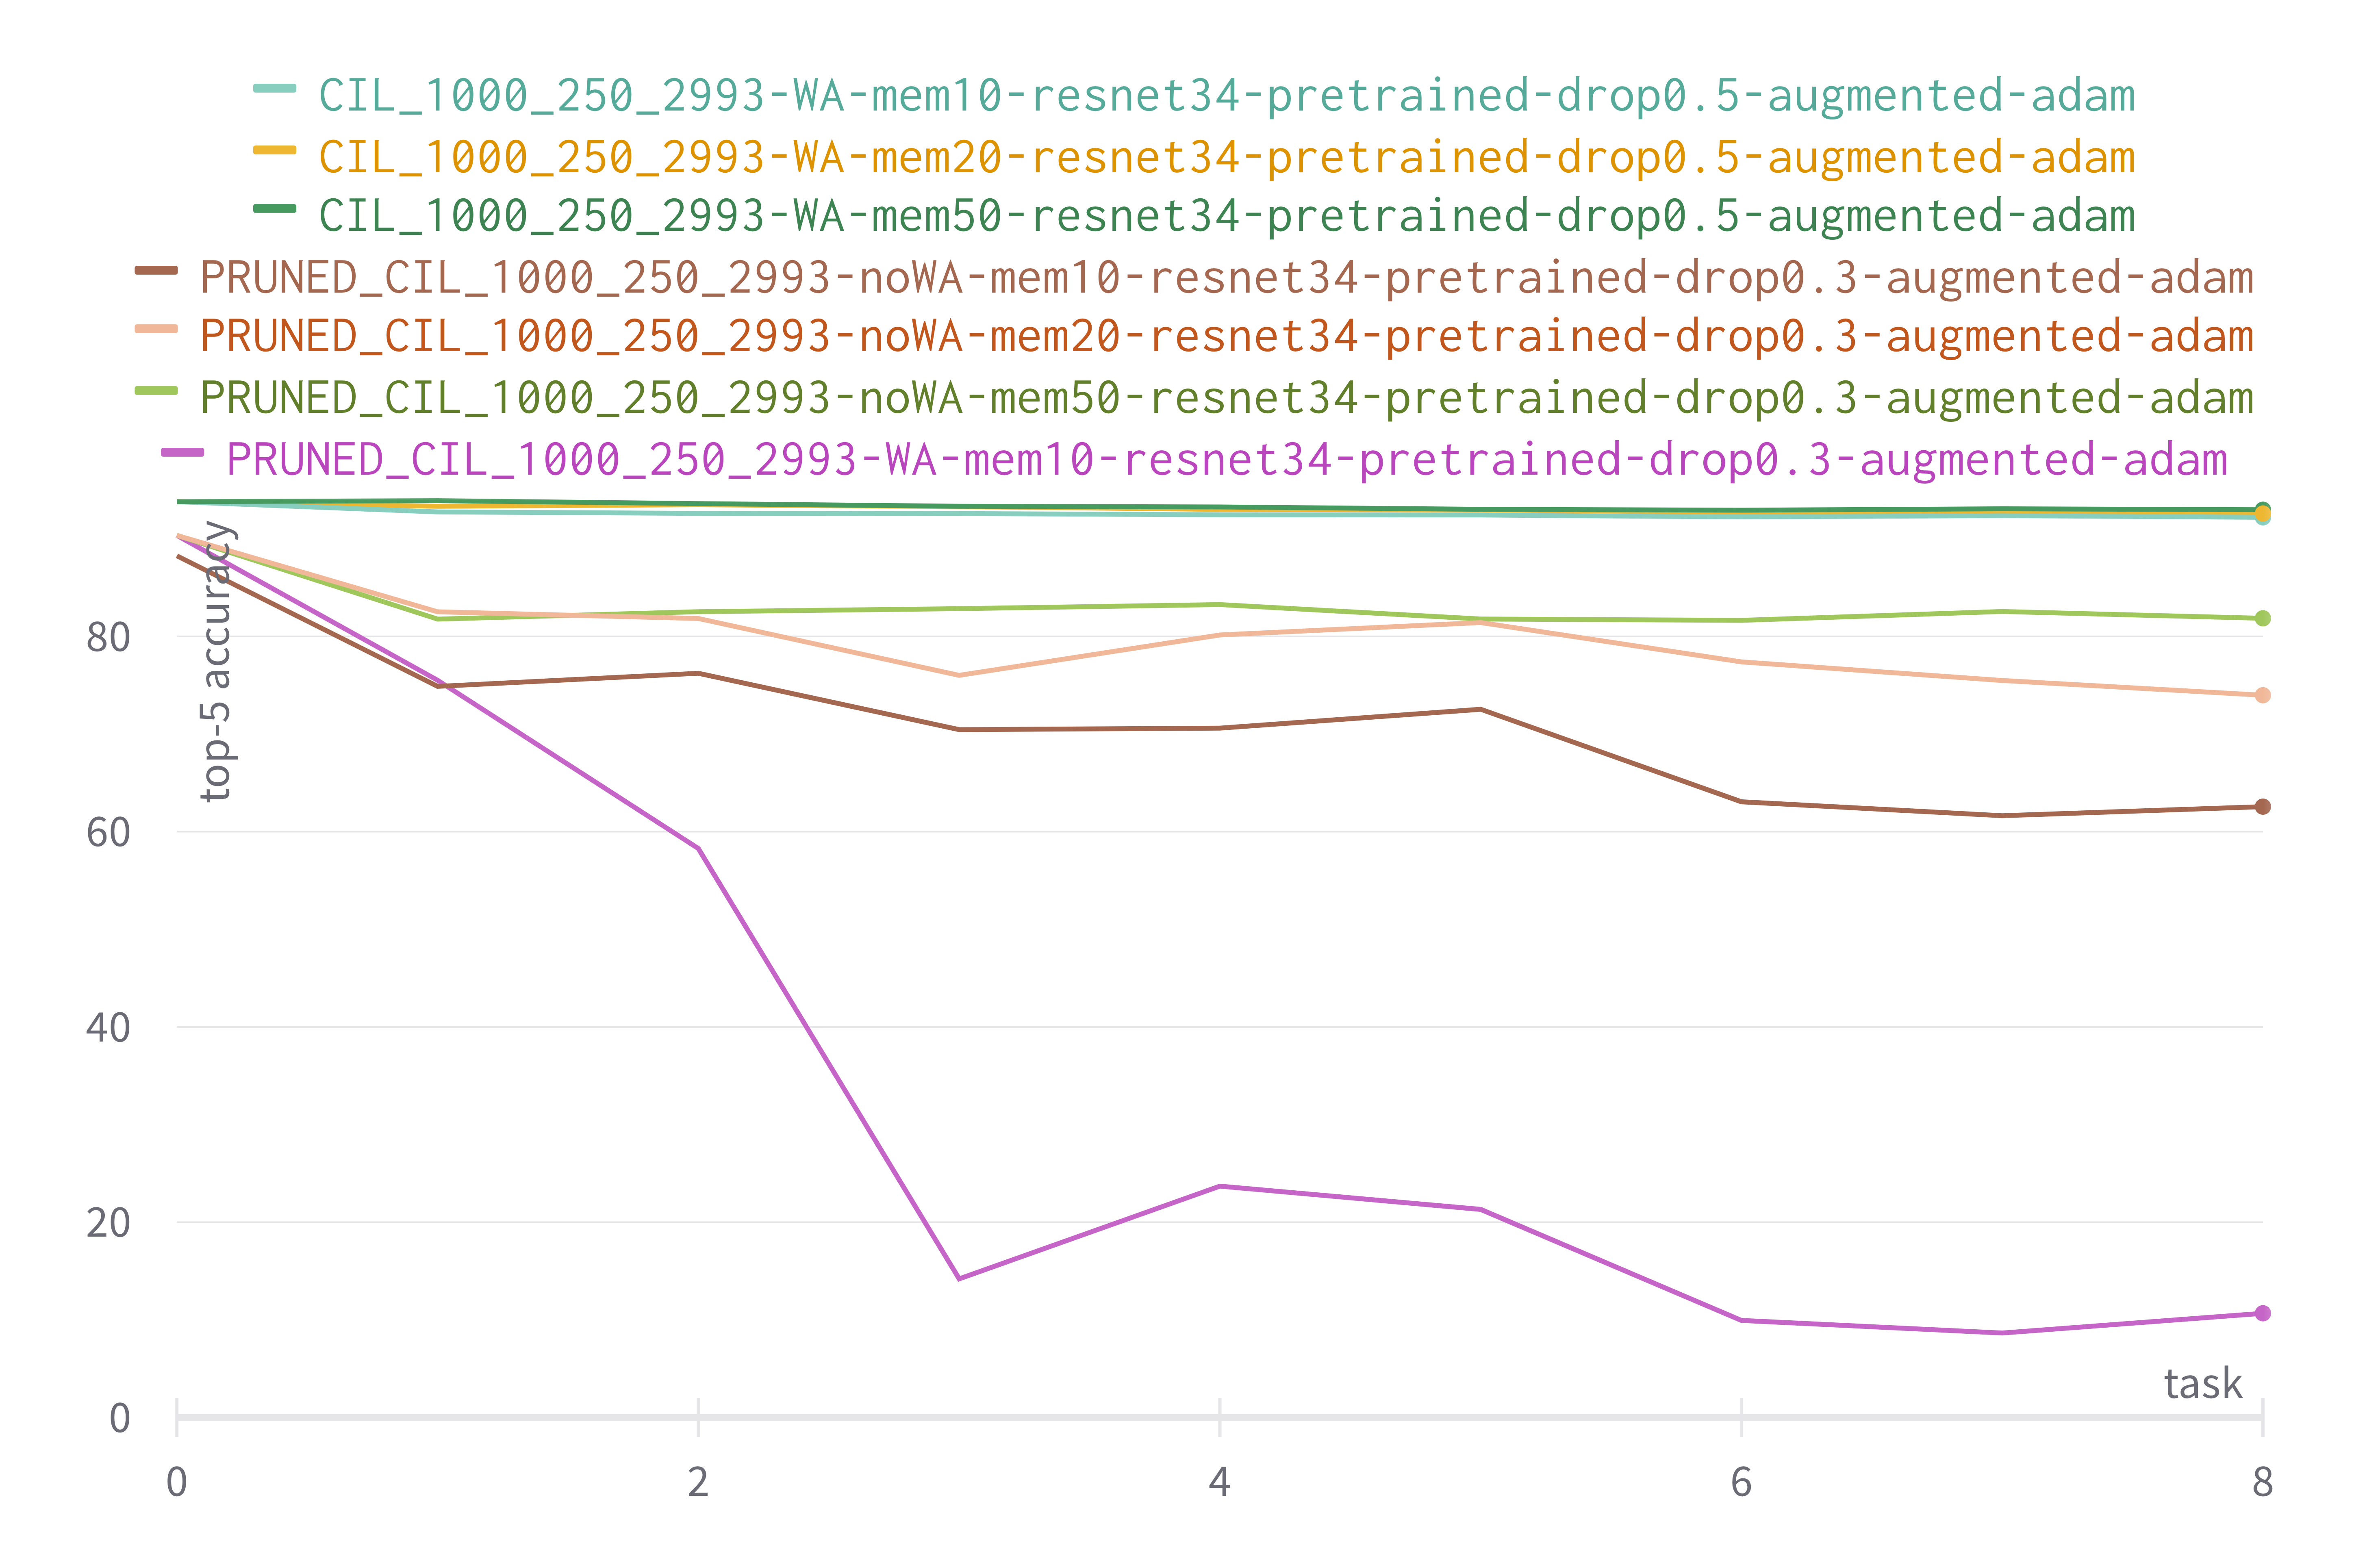
\includegraphics[width=0.80\textwidth]{images/exp/exp7-top5.png} }}%
	\caption{Performance comparison between the pruned and unpruned models trained on the entire dataset.}%
	\label{fig:exp7}
\end{figure}

\newpage

\section{Knowledge Distillation}
\label{sec:exp-kd}
To address the drastic drop in accuracy when using pruning on models trained on the whole dataset (see \autoref{sec:pruning-entire}), KD is adopted as described in \autoref{sec:method-kd}. During the KD, an un-pruned model is used as the teacher, while the student is a significantly smaller CNN. In the experiments presented in this section, ResNet-50 pretrained on ImageNet is used as the backbone for the student, with a dropout layer before the FC layer.

KD is performed after the training of the teacher model. Since the CIL classifier is trained using the DER algorithm, and this algorithm requires that a part of the examples of the old classes is stored, in a real situation the KD can only be performed with those examples available as a result of the storage. For this reason, in order to reproduce a realistic situation, the student model is trained under the supervision of the teacher, but only the samples stored by the teacher are used as training data.

The result of the experiments regarding KD are shown in \autoref{table:exp-kd}, where different models with varying memory size are used as teachers. As we can see, the number of examples used to train the student heavily affects the final performance.
However, the student trained with 50 samples per class achieves 0.80 as top-1 accuracy, resulting in performance drop of 9\% compared to the teacher model. Although this drop in performance is rather large, it is important to consider the number of parameters: all teacher models have 205 million parameters, while the final models used as students have 30 million parameters.
Therefore, even if the accuracy drops, the number of parameters drops by a factor of almost 7x.

KD outperforms the result obtained with the pruning method (see \autoref{table:exp7} and \autoref{table:exp7-params}). In fact, comparing KD with pruning, the performance increases from 70.37\% to 80.0\% and the compression factor goes up from 3x to 7x.


\begin{table}[H]
    \centering
    \begin{tabular}{c|c|c|c|c}
        \hline
        \textbf{Teacher} &
        \textbf{Student} &
        \textbf{Mem.} &
        \textbf{Dropout rate} &
        \textbf{Top-1} \\
        \textbf{model} &
        \textbf{model} &
        \textbf{size} &
        \textbf{student} &
        \textbf{acc. (\%)} \\
        \hline
        \hline
UNPRUNED-WA-mem10-drop0.5&ResNet-50&10&0.1&62.42\\
UNPRUNED-WA-mem50-drop0.5&ResNet-50&10&0.3&69.09\\
UNPRUNED-WA-mem50-drop0.5&ResNet-50&50&0.3&\textbf{80.0}\\
\hline
\end{tabular}
\caption{Top-1 accuracy of the students trained using KD. The teacher column represents which model is used as teacher, the student column refers to the backbone of the student model. }
    \label{table:exp-kd}
\end{table}


\section{Logo detector}
\label{sec:exp-det}
This section described the experiments designed to evaluate the class-agnostic logo detector introduced in \autoref{sec:method-roi}.
The CIL classifier is trained starting from the cropped regions.
However, the detector predicts the bounding boxes using the entire image as input.
Since an image can contain multiple logos, the detector is trained to exploit the same training, validation and testing set used by the CIL classifier.
This is done by considering the training labels for the detector only if that bounding box corresponds to a ROI used as a training example for the classifier, otherwise the bounding box is used in the validation or test set, depending on the split used for the classifier.
This process is shown in \autoref{fig:detector-split-dataset}.
This results in an unbiased evaluation of both the detector and the classifier.

\begin{figure}[H]
	\centering
    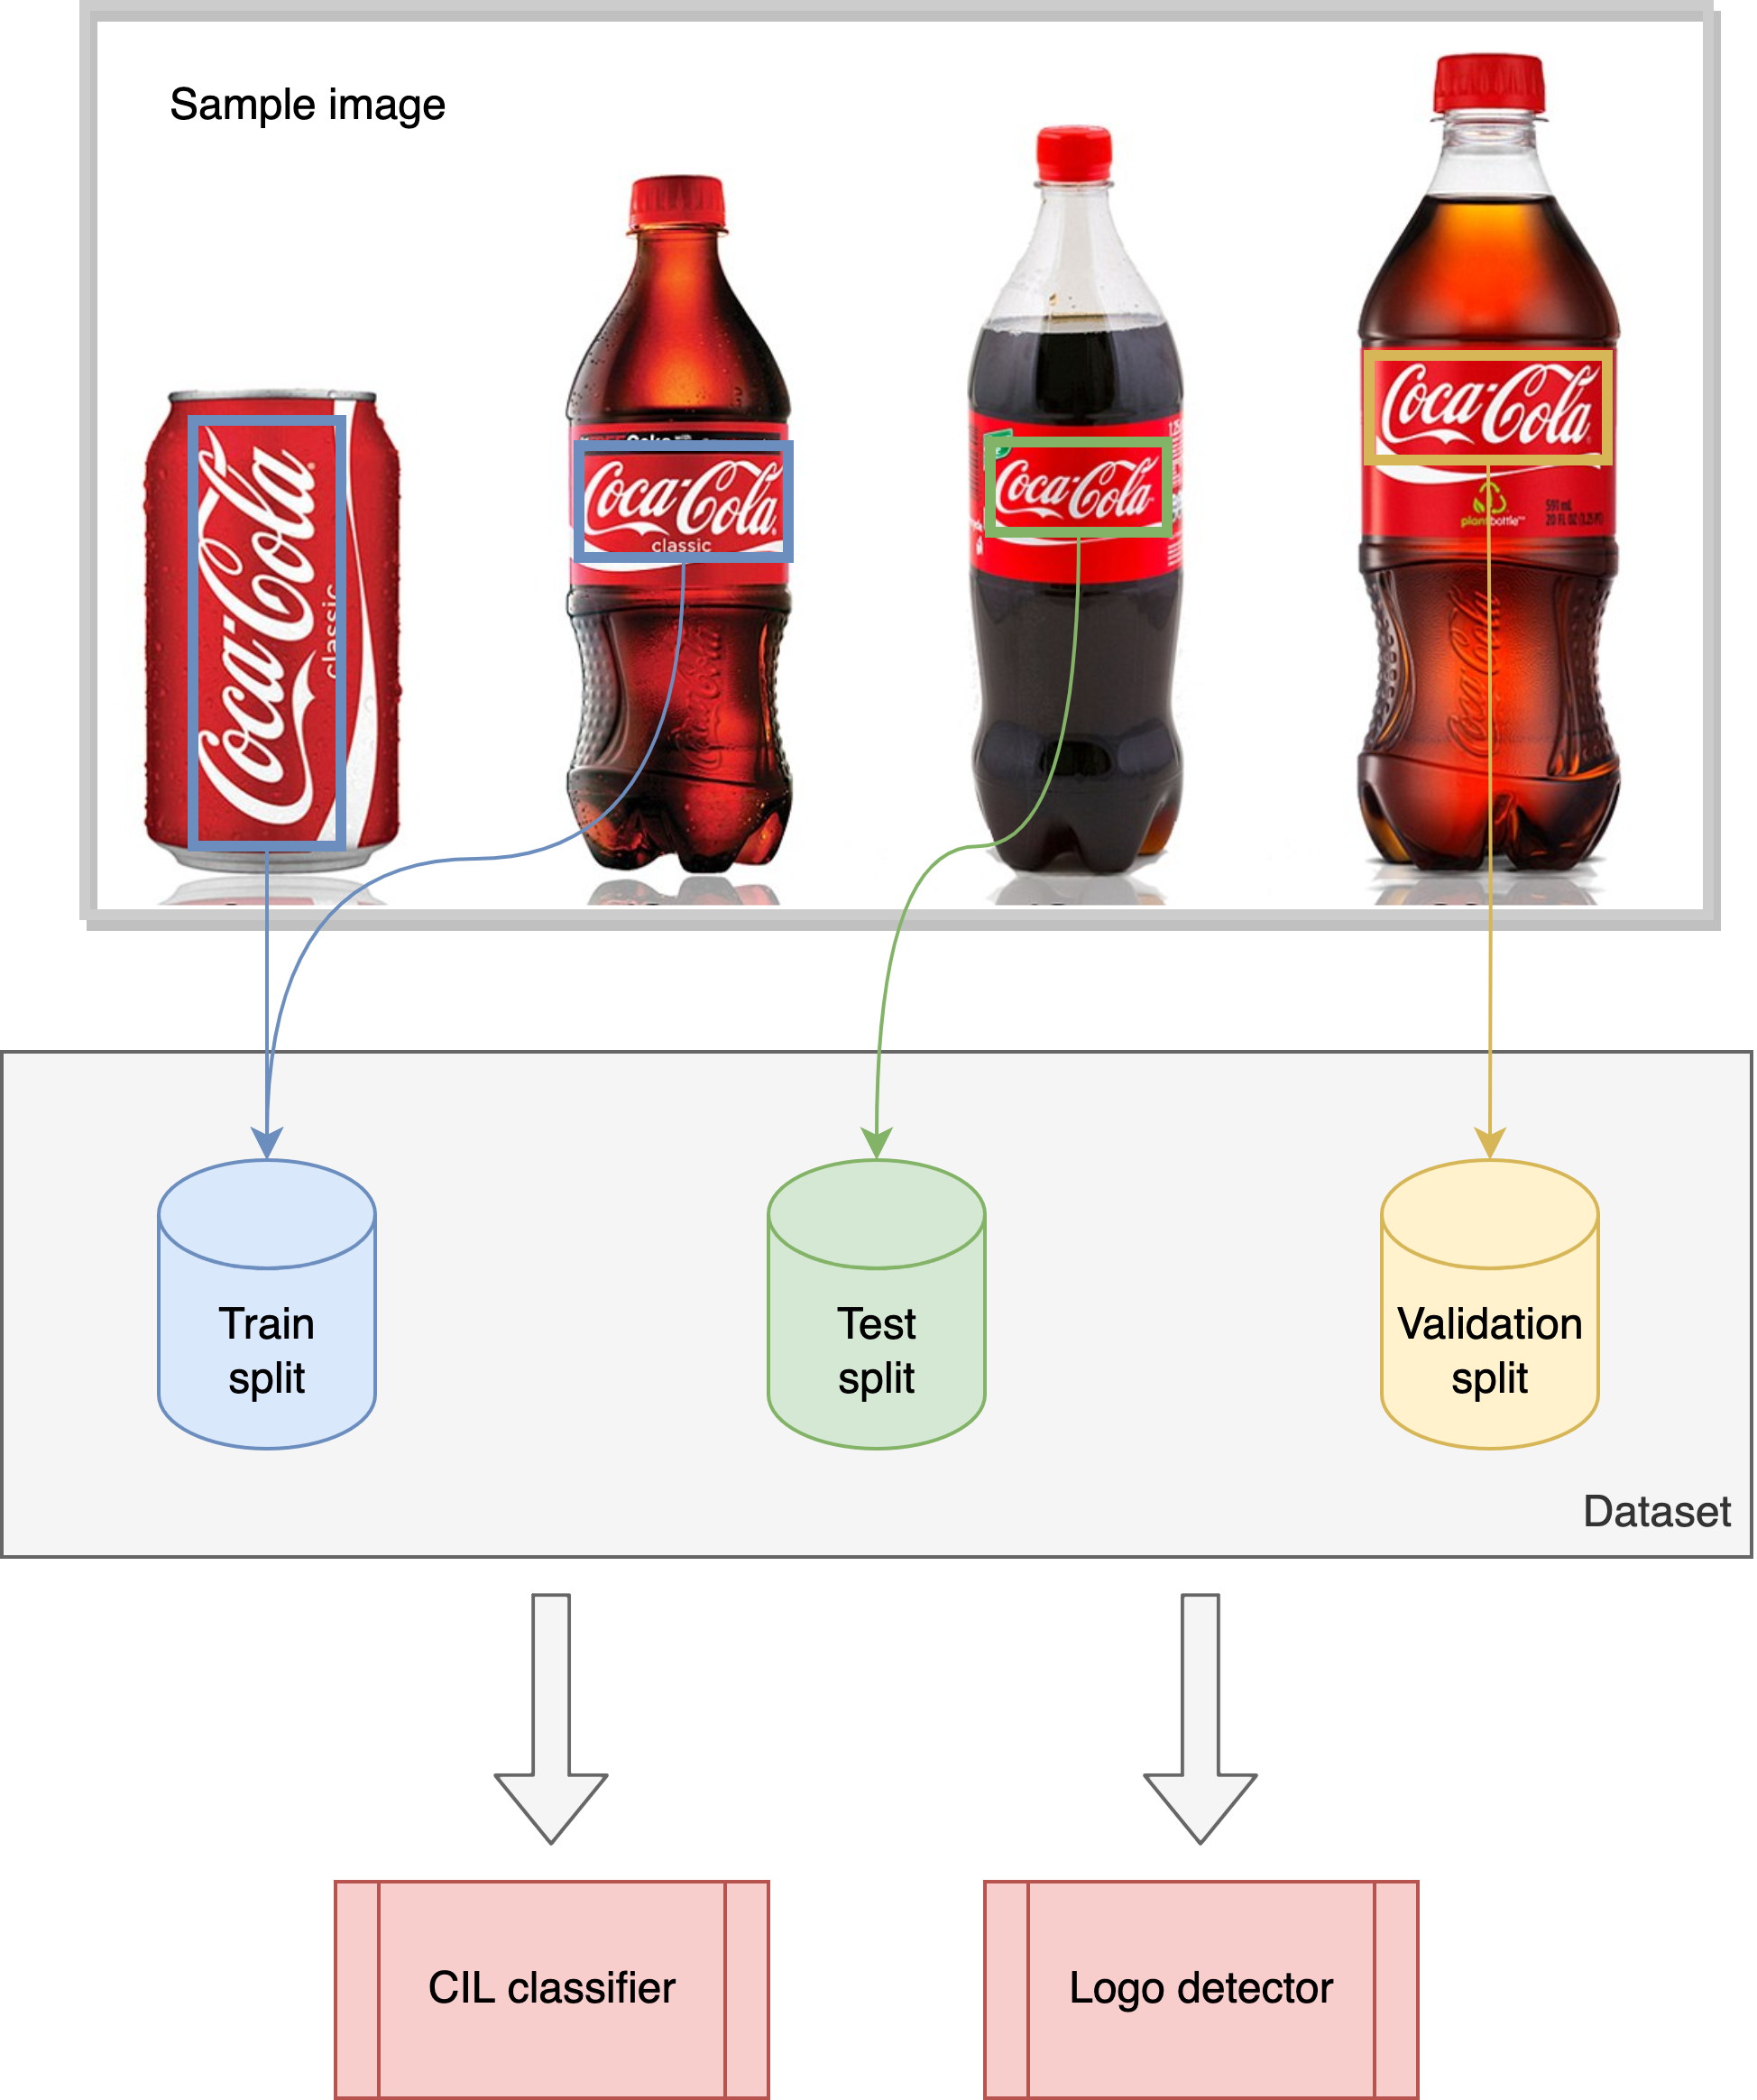
\includegraphics[width=0.7\textwidth]{images/logos-split.drawio.png}
	\caption{Training, validation and test split for the detector based on the splits used to train the CIL classifier.}%
	\label{fig:detector-split-dataset}%
\end{figure}

\subsection{Metrics}
Mean Average Precision (mAP) metric is a metric used to evaluate object detection models. This metric is based on: Intersection over Union (IoU), Recall, Precision.

\subsubsection{Intersection over Union}
Given a ground-truth bounding box $box_{gt}$ and a detected bounding box $box_{pred}$, as shown in \autoref{fig:iou}, the IoU is computed as the ratio of the overlap and union areas:
\begin{equation}
    \text{IoU} = \frac{box_{gt} \cap box_{pred}}{box_{gt} \cup box_{pred}} 
\end{equation}
Then a prediction is considered correted if IoU $ \geq \tau$, where $\tau$ is a threshold (a typical value for $\tau$ is $0.5$).

\begin{figure}[H]
	\centering
    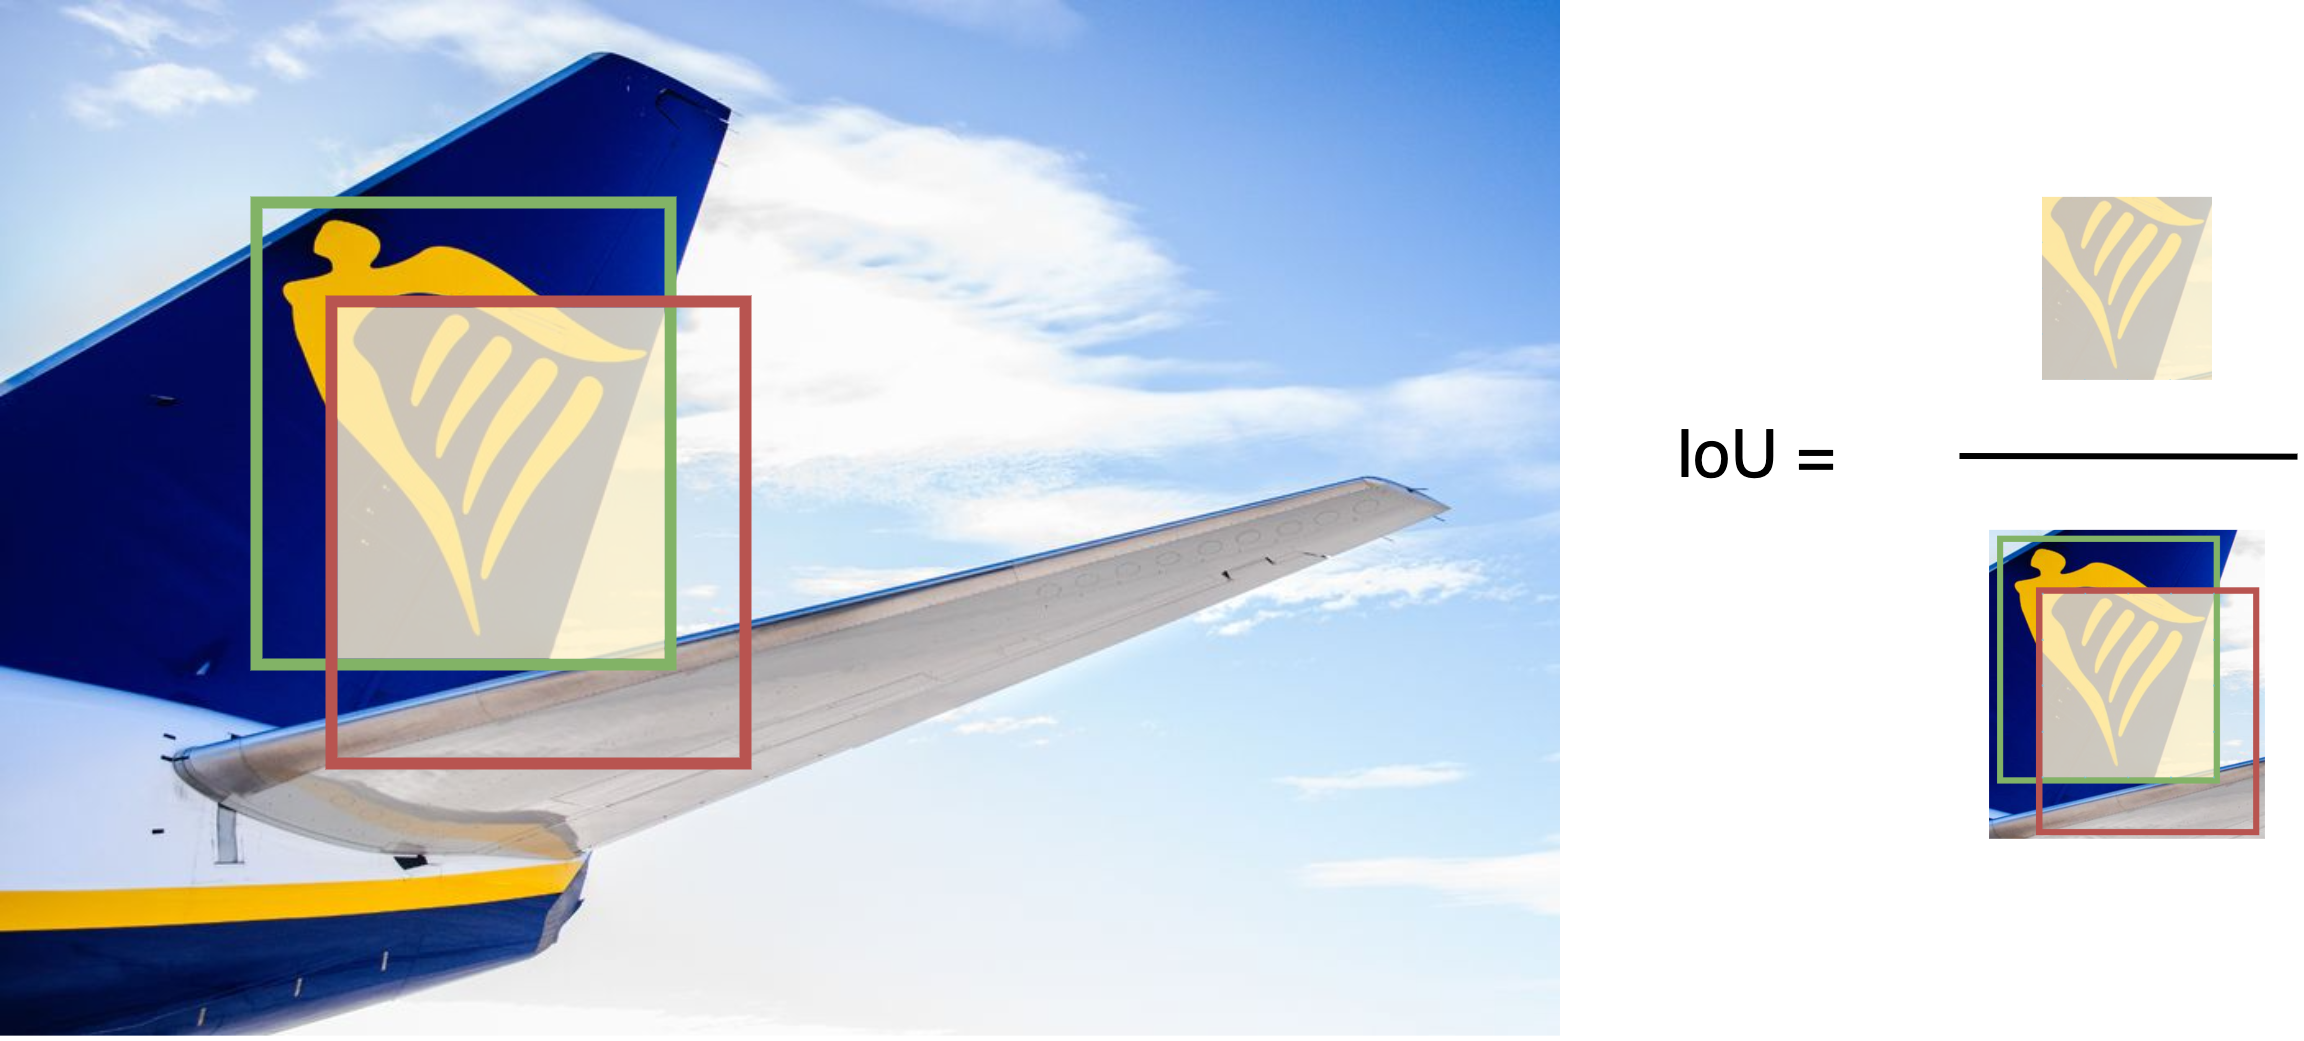
\includegraphics[width=1\textwidth]{images/iou.drawio.png}
	\caption{Intersection over Union (IoU). The green box represents the ground-truth bounding box, the red one represents the predicted bounding box and the intersection is given by the yellow region. Then, the IoU is computed as the ratio of the overlap and union areas.}
	\label{fig:iou}
\end{figure}

\subsubsection{Precision and Recall}
Given the IoU and a threshold $\tau$ it is possible to count the number of:
\begin{itemize}
    \item True Positive (\textbf{TP}): The number of bounding boxes which have a IoU $geq \tau$ with the ground-truth bounding box.
    \item False Positive (\textbf{FP}): The number of bounding boxes that predict an object which is not actually an object.
    \item False Negative (\textbf{FN}): The number of bounding boxes which have a IoU $< \tau$ with the ground-truth bounding box.
\end{itemize}
Note that the True Negative (TN) are not considered in an object detection task, as this would mean counting as TN the background of the image that contains no object.

Then, the Precision $P$ is given by:
\begin{equation} %tp / (tp + fp)
    P = \frac{TP}{TP + FP}
\end{equation}
and the Recall $R$ is given by:
\begin{equation} %tp / (tp + fn)
    R = \frac{TP}{TP + FP}
\end{equation}
Intuitively, precision is the ability of the detector not to consider as object a part of the image that is not, and recall is the ability of the detector to find all objects in the image.
The threshold $\tau$ affects the number of TP, FP, FN, thus the value of Precision and Recall. For this reason, given a value for $\tau$ (e.g. $\tau = 0.5$), when computing the Precision/Recall at $\tau = 0.5$, this is denoted by $P@.5$ and $R@.5$.

\subsubsection{Mean Average Precision}
Average Precision (AP) is calculated as the weighted mean of precisions at each threshold; the weight is the increase in recall from the prior threshold. For values of $\tau \in T$, where $T = [0.50, 0.55, 0.60,\, ..., \, 0.95 ]$, the AP computed using the thresholds in $T$ and denoted by $\text{AP}@.5:.95$ is given by:
\begin{equation}
    AP = 1 \sum_{i=1}^{|T| - 1}(R@\tau_i - R@\tau_{i+1} ) * P@\tau_{i}
\end{equation}
Finally, given $k$ different classes, the mAP is the average of the AP among each class:
\begin{equation}
    mAP = \frac{1}{k} \sum_{i=1}^{k} AP_i
\end{equation}

\subsection{100 Classes}
As in the case of the CIL classifier, the logo detector is initially trained using the top-100 classes of the dataset (where top-100 refers to the 100 classes with the highest number of samples, see \autoref{sec:cil-top100}).

As described in \autoref{chap:methods}, the class-agnostic logo detector represents the first stage of the system and works in combination with the CIL model to achieve incremental learning logo detection and recognition. Given the nature of the problem, in a real case scenario, the detector is trained using only those classes available for the CIL model at task 0. In the experimental setup described in \autoref{sec:exp-setup}, the initial task consists in 30 classes.

For this reason, in the top-100 classes setup, the detector is trained for 30 epochs with the SGD optimizer using only those 30 classes available at task 0.
Note that, as described at the beginning of this section, the 30 classes correspond to those considered by the CIL model at task 0. Furthermore, the train, validation and test sets  for the detector are maintained identical as the classifier, so that to use the same sample images for training and testing of the two models

During the training of the detector, the object loss, box loss (see \autoref{sec:yolo} and \autoref{eq:yolo-loss}) and the mAP@.5 is monitored on the validation set. The performance shown in \autoref{fig:exp-det_100} considers only the 30 classes used for training, which is a useful information for analyzing the training phase. However, considering an incremental learning setup, we expect the class-agnostic logo detector to perform well on all the 100 classes.
To this purpose, the detector is evaluated considering the mAP@.5 on the test set of the initial 30 classes and the test of the remaining 70 classes.
This evaluation represents a real-world scenario and it is therefore the most reliable performance and best suited to assessing the detector.
The result of the evaluation is shown in \autoref{table:exp-det_100}.

To better investigate the generalizing capabilities of the detector trained on 30 classes to the remaining 70, the detector is compared with a new one trained on all the 100 classes.
This detector can be considered as a baseline with regard to the generalization capabilities of the detector trained on 30 classes: the smaller the gap between the performance of these two models, the better the generalization capabilities.
This new detector is trained for 30 epochs on the 100 classes and, as before, the object loss, box loss and the mAP@.5 is monitored on the validation set. The comparison between the two detector is shown in \autoref{fig:exp-det_100}.

As we can see from \autoref{fig:exp-det_100}, the performance between the detectors trained on 100 and 30 classes are quite similar. However, a crucial aspect of this training results, is that these metrics consider all and only the classes which the model is trained on, thus 30 classes and 100 classes.
The fact that the detectors achieve the same performance is a sign that they accomplish similar results in detecting logos across a different number of classes.
However, the real comparison consists in considering the mAP@0.5 for each detector, computed on the test set of all the 100 classes. This comparison is shown in \autoref{table:exp-det_100}.

From \autoref{table:exp-det_100}, we can see how the detector trained on 30 classes does not generalize well on the remaining 70 classes.
In fact, comparing the mAP@.5 computed on the test set composed of all the 100 classes, with the mAP@.5 obtained on the validation in the last epochs of training (shown in \autoref{fig:exp-det_100}), the drop in performance goes from about 0.97 to 0.75.

In contrast, the detector trained on all the 100 classes, obtains a mAP@.5 on the test set of 0.982, which is consistent with the performance obtained on the validation set in the last epochs of training.
However, it must be considered that, as this detector is trained using 70 more classes, it has more training samples at its disposal, hence more data from which to acquire knowledge of a logo.


\begin{table}[H]
    \centering
    \begin{tabular}{c|c|c|c|c}
        \hline
        \textbf{Model} &
        \textbf{Precision} &
        \textbf{Recall} &
        \textbf{mAP@.5} &
        \textbf{mAP@.5:.95} \\
        \hline
        \hline
DET\_class-agnostic\_30cls&0.784&0.659&0.75&0.542\\
DET\_class-agnostic\_100cls&0.944&0.972&0.982&0.776\\
\hline
\end{tabular}
\caption{Precision, Recall, mAP@.5 and mAP@.5:.95 obtained by the detector trained on 30 classes (DET\_class-agnostic\_30cls) and that trained on 100 classes(DET\_class-agnostic\_10cls). The performance refers to the test set composed of all the 100 classes.}
    \label{table:exp-det_100}
\end{table}

\begin{figure}[H]
	\centering
	\subfloat[\centering mAP@.5]{{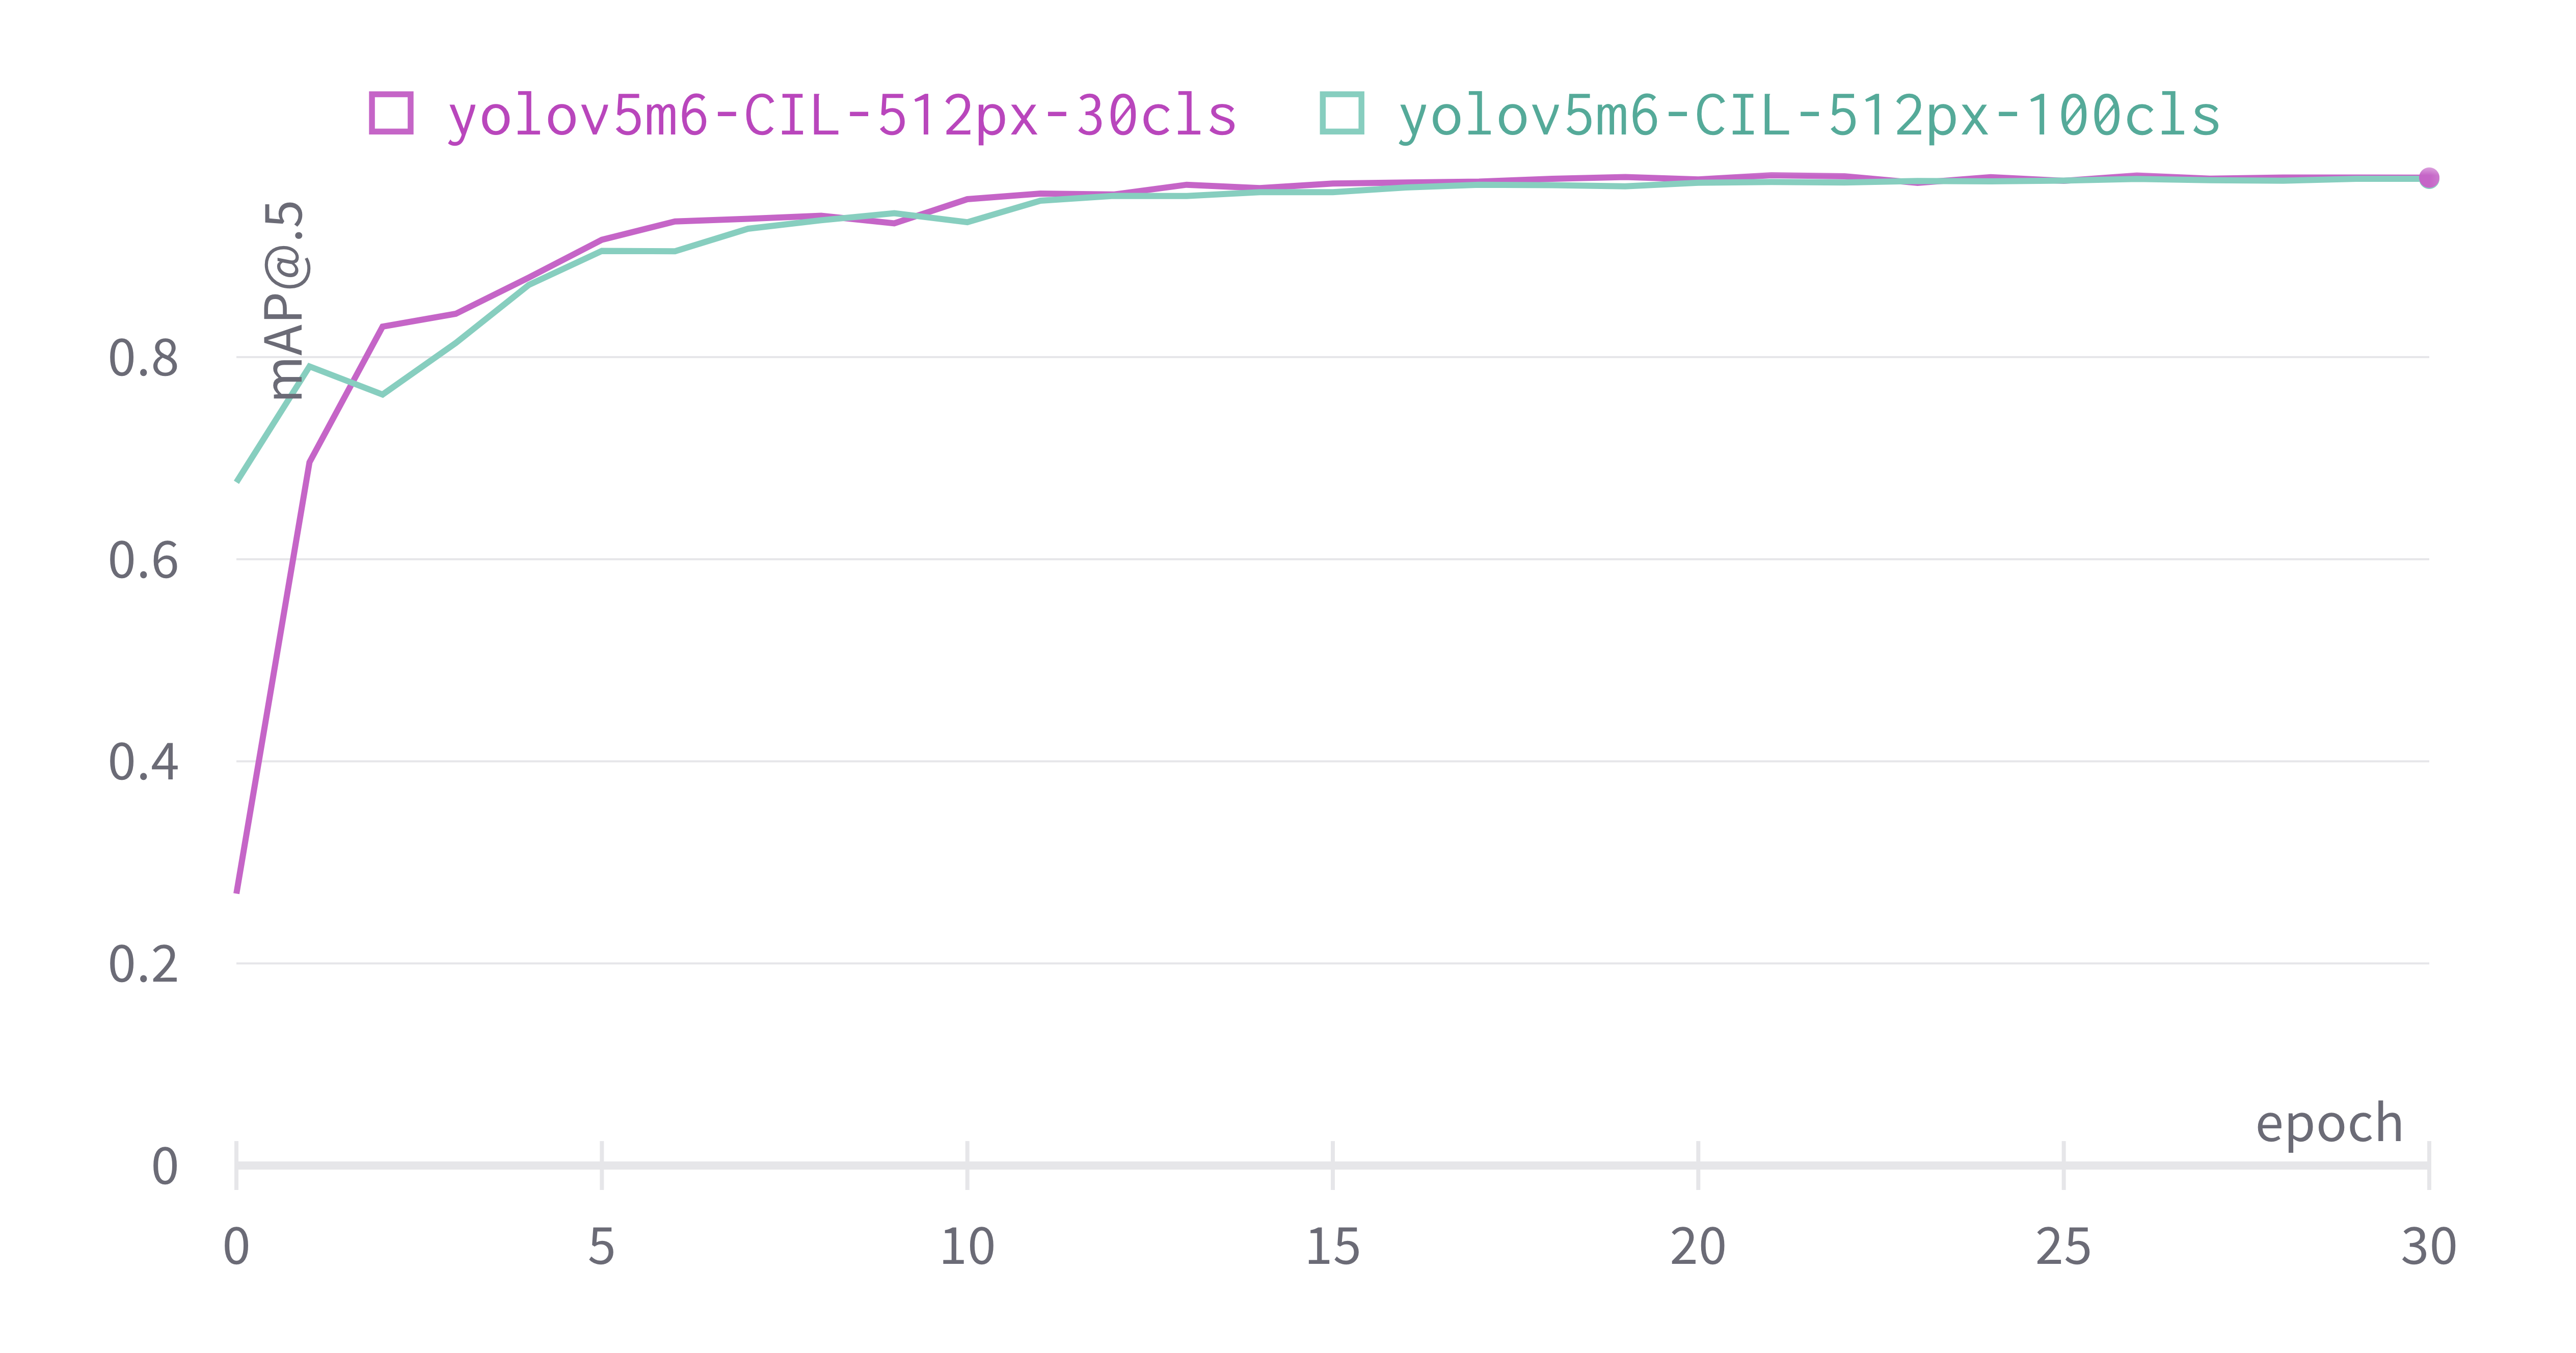
\includegraphics[width=0.70\textwidth]{images/exp/exp-det-map.png} }}%
    \qquad
	\subfloat[\centering Box loss]{{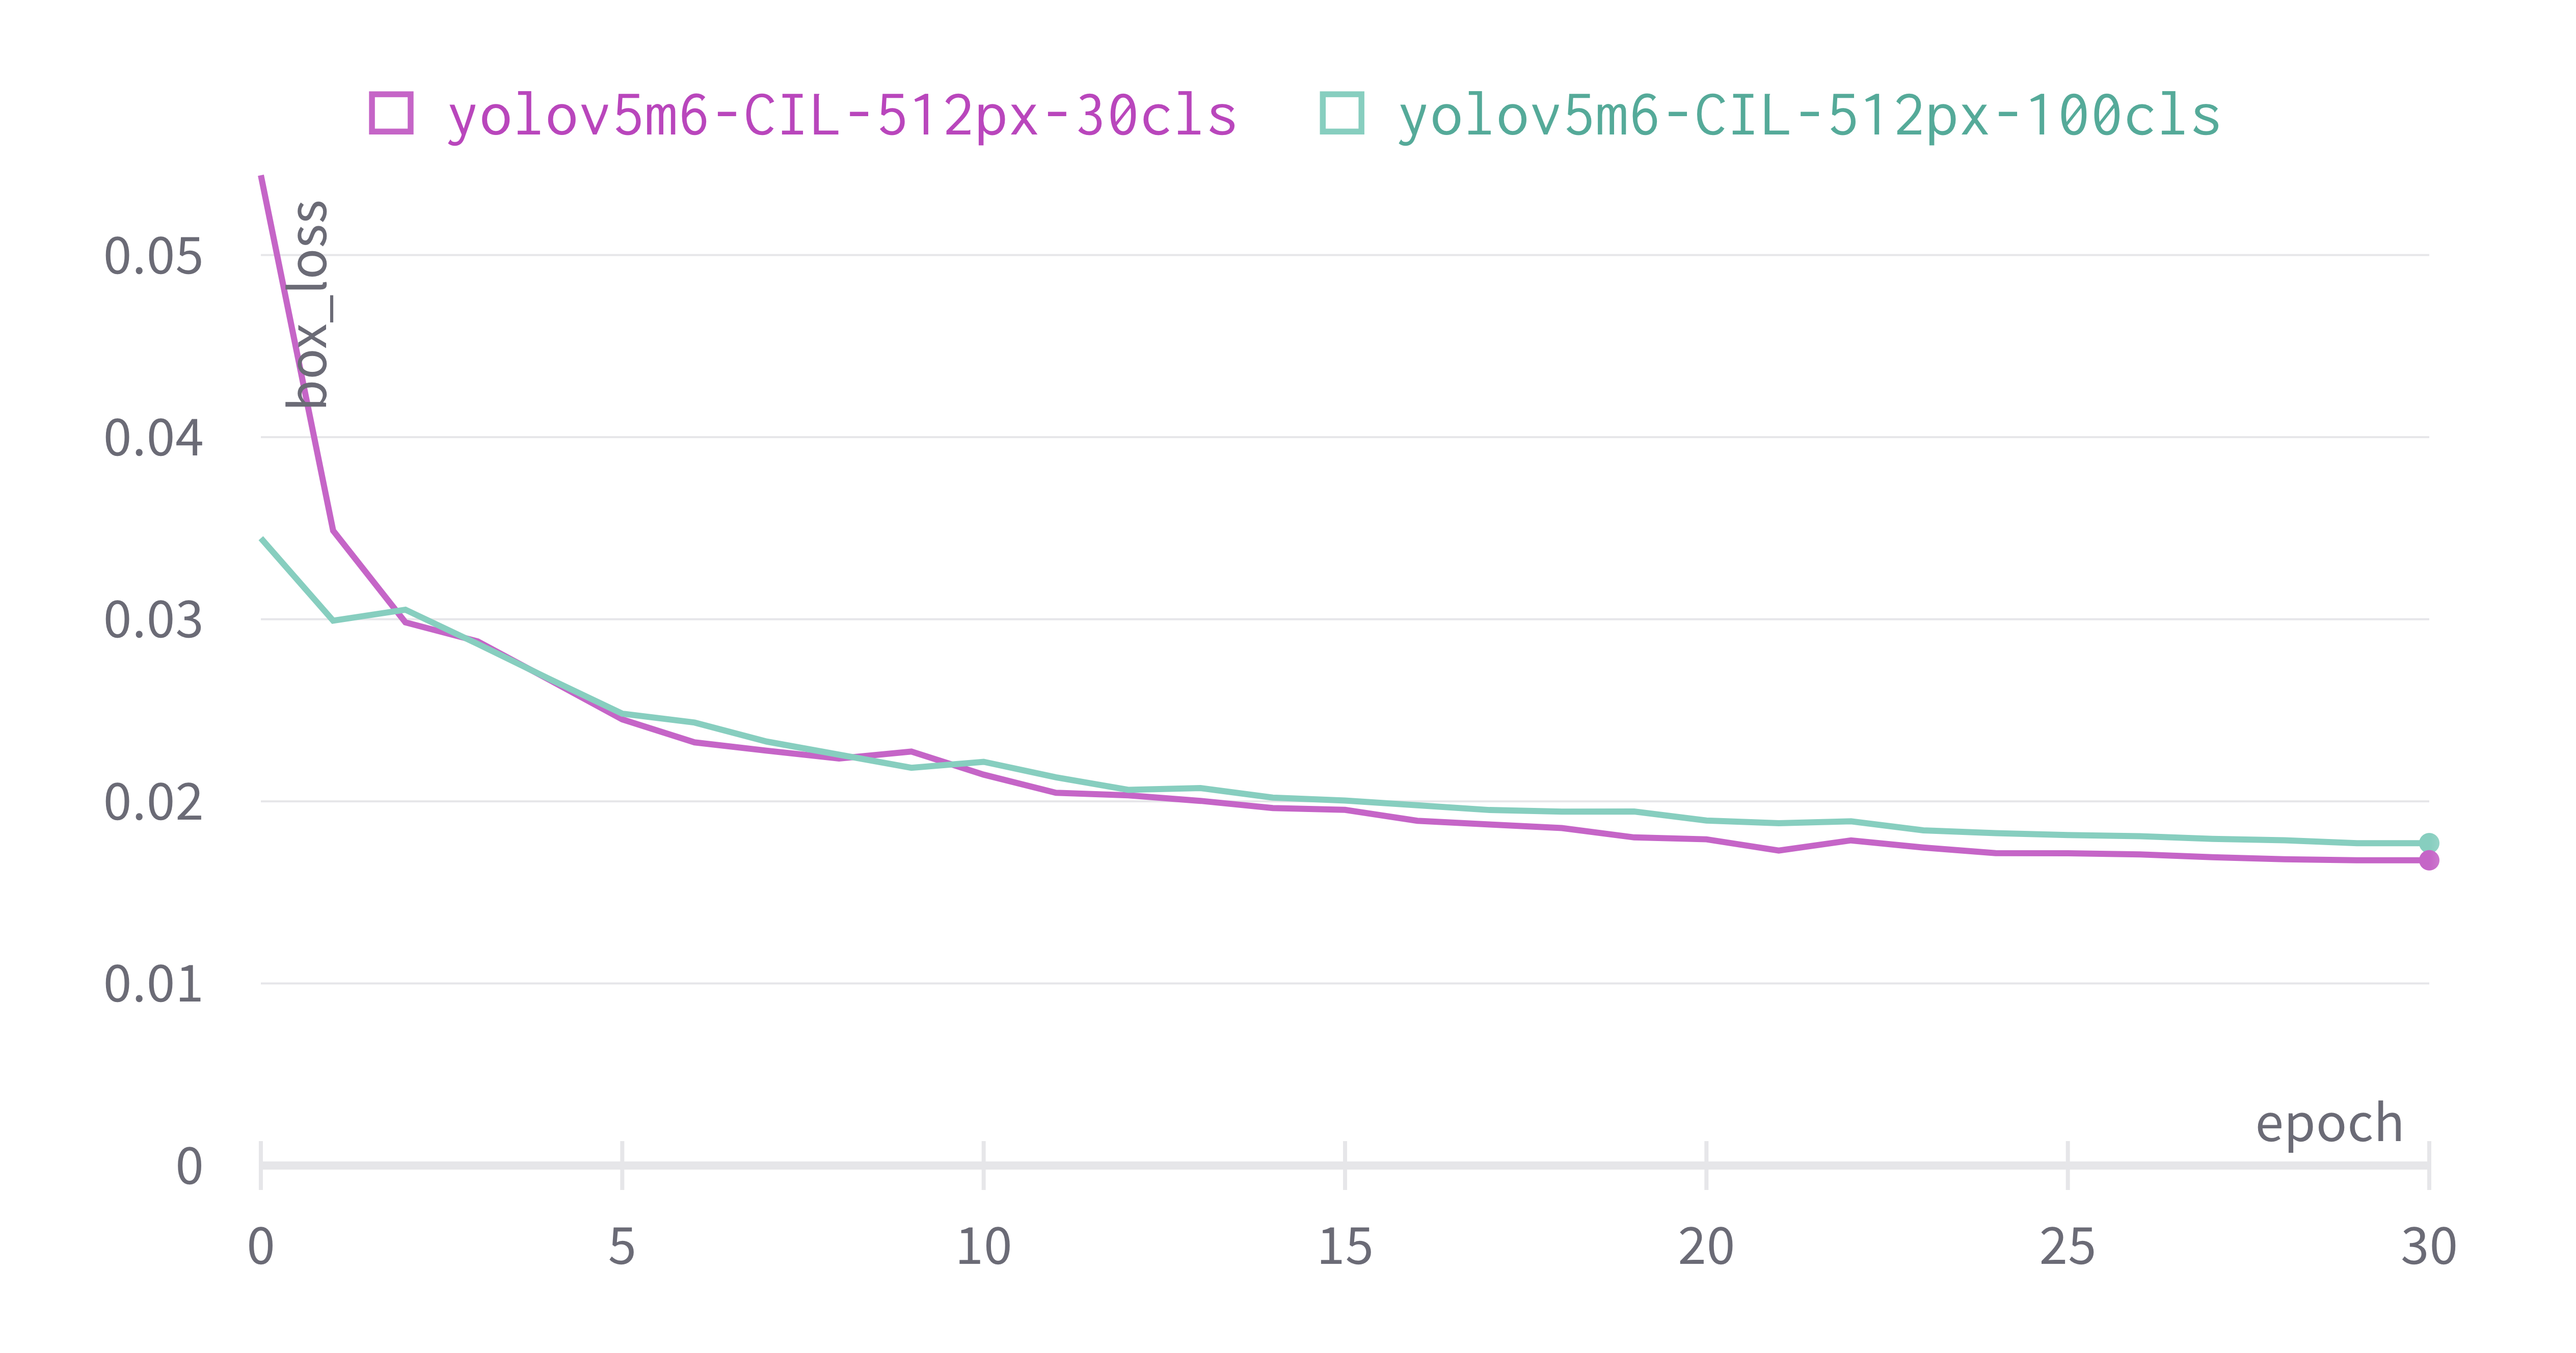
\includegraphics[width=0.70\textwidth]{images/exp/exp-det-box_loss.png} }}%
    \qquad
	\subfloat[\centering Obj loss]{{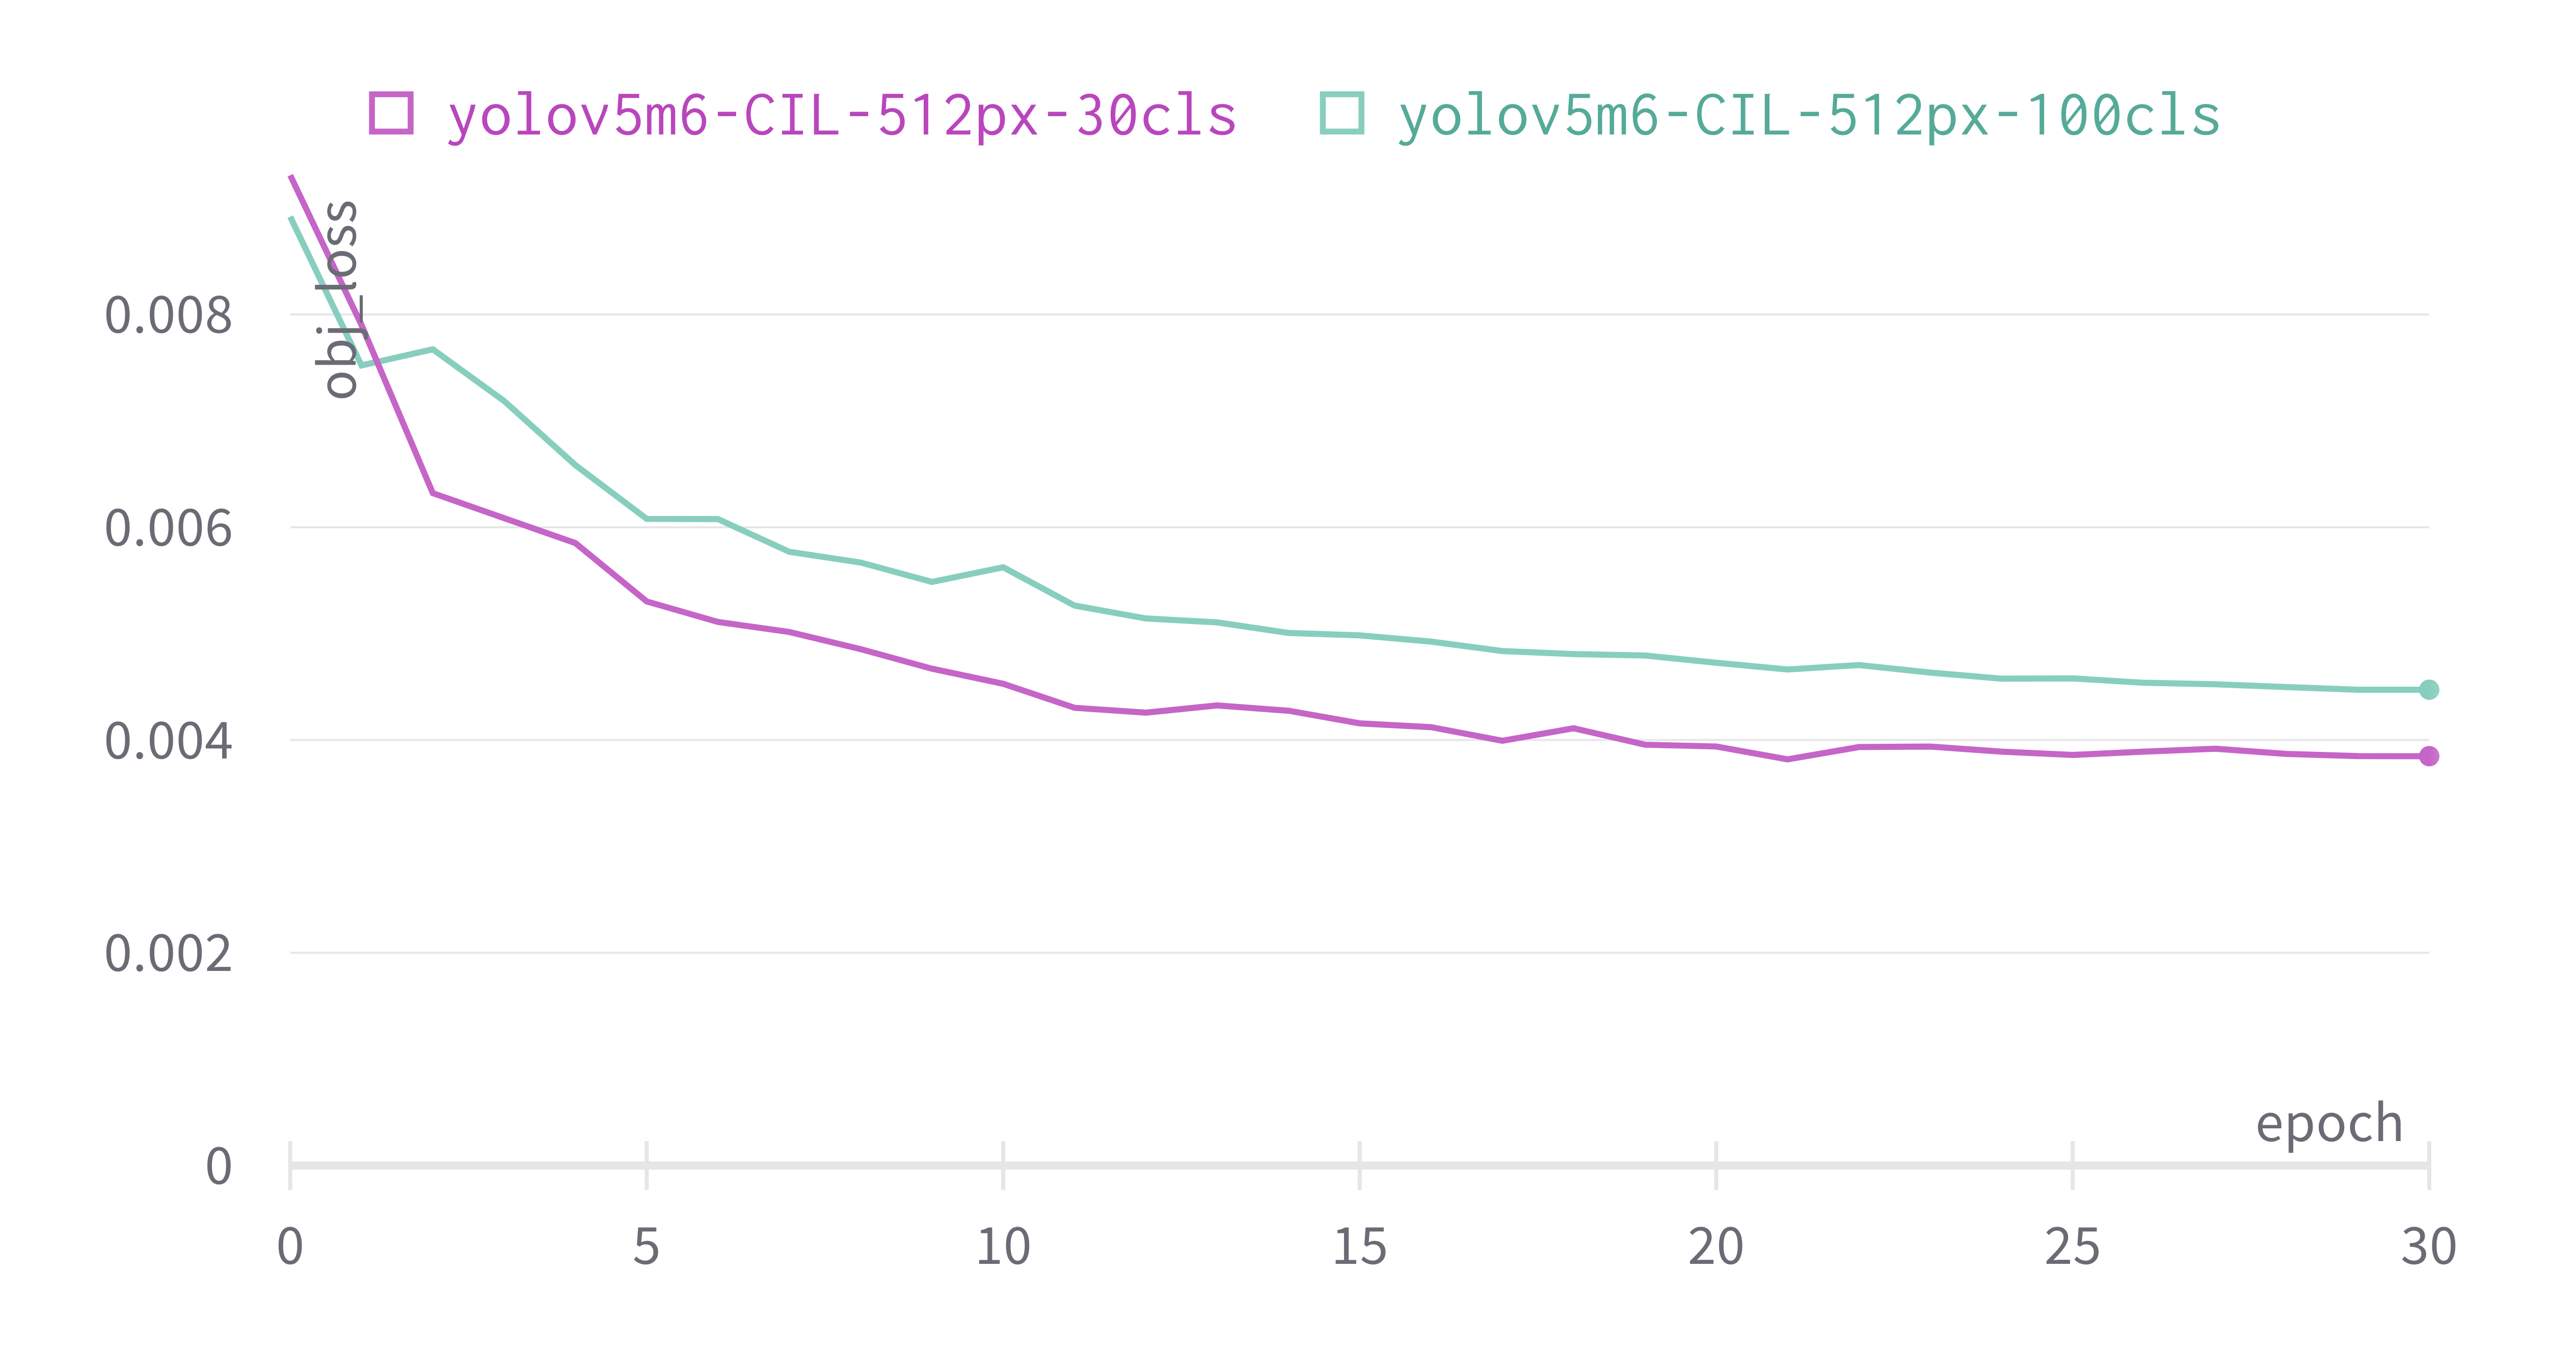
\includegraphics[width=0.70\textwidth]{images/exp/exp-det-obj_loss.png} }}%
    \caption{Performance comparison between the class-agnostic logo detector trained on 30 classes and the one trained on 100 classes. The plots show the mAP@.5, box loss and object loss on the validation set at each training epoch. Note that these performance are computed on the validation set of each model, thus using 30 and 100 classes respectively.}%
	\label{fig:exp-det_100}
\end{figure}


\subsection{2993 Classes}
\subsubsection{Ablation study}
WA non utilizzato ma non peggiora molto le cose, probabilemnte perchè ci sono pochi esempi quindi qeusto non affect molto.


\section{End to end classification}
\label{sec:exp-end2end}
